\documentclass[11pt,a4paper]{article}
\usepackage[margin=2.1cm]{geometry}
\usepackage{lmodern}
\usepackage[T1]{fontenc}
\usepackage{graphicx}
\usepackage{booktabs}
\usepackage{longtable}
\usepackage{array}
\newcolumntype{L}[1]{>{\raggedright\arraybackslash}p{#1}}
\usepackage{amssymb}
\usepackage{xcolor}
\usepackage{listings}
\usepackage{float}
\usepackage{caption}
\usepackage{enumitem}
\usepackage{tikz}
\usetikzlibrary{arrows.meta,positioning,shapes.geometric}
\usepackage[most]{tcolorbox}
\usepackage[colorlinks=true,linkcolor=blue!50!black,urlcolor=blue!50!black,citecolor=blue!50!black]{hyperref}

\definecolor{codebg}{RGB}{247,247,245}
\definecolor{keyw}{RGB}{42,120,214}
\definecolor{strc}{RGB}{0,131,0}
\lstdefinestyle{py}{language=Python,basicstyle=\ttfamily\scriptsize,backgroundcolor=\color{codebg},
  keywordstyle=\color{keyw}\bfseries,stringstyle=\color{strc},commentstyle=\color{gray},showstringspaces=false,
  frame=single,rulecolor=\color{gray!40},breaklines=true,columns=fullflexible,aboveskip=4pt,belowskip=4pt}
\lstdefinestyle{plain}{basicstyle=\ttfamily\scriptsize,backgroundcolor=\color{codebg},frame=single,
  rulecolor=\color{gray!40},breaklines=true,columns=fullflexible}
\newtcolorbox{keybox}[1]{colback=blue!3,colframe=blue!40!black,fonttitle=\bfseries,title=#1,boxrule=0.6pt,arc=2pt}
\newtcolorbox{warnbox}[1]{colback=orange!4,colframe=orange!60!black,fonttitle=\bfseries,title=#1,boxrule=0.6pt,arc=2pt}
\setlist{itemsep=2pt,topsep=3pt}
\captionsetup{font=small}
\sloppy

\title{\textbf{TopoGraph: teaching LLMs to draw the dataflow graph of PyTorch code}\\[4pt]
\large An explainer of the whole project: data, code, journey, results, examples and caveats}
\author{IE 643 (IIT Bombay, Autumn 2026)\\Team MachineUnlearning: Devanshu Jha \& Peela Rathna Harsha\\
\small Written from the project repository (code, logs and result files in \texttt{IE643\_Project/topograph})}
\date{25 October 2026}

\begin{document}
\maketitle

\begin{keybox}{The project in one paragraph}
Given the source code of a PyTorch \texttt{nn.Module}, a large language model (LLM) must write down the
\emph{forward-pass dataflow graph} of that module: one node per layer or operation, one edge per tensor that flows
between them, plus each node's kind and output tensor shape. The exact answer is computed by \texttt{torch.fx}, so we
can grade every prediction automatically. We built the full pipeline (data splits, a reference ``oracle'', a validator
that checks a graph \emph{without} knowing the answer, many metrics, a graph drawer, LoRA fine-tuning, fast inference
with constrained decoding and self-correction, an evaluation suite and a demo app) and ran 30+ experiments with
Qwen3.5 (0.8B--27B) and Qwen2.5-Coder-7B. \textbf{Main result:} fine-tuning makes a 9B model essentially perfect on
the dataset's own distribution (99.7\% valid, 100\% on held-out topologies), but it breaks on genuinely new code
(47.5\% on our hand-written out-of-distribution set). Adding $\sim$2{,}800 randomly generated, automatically labelled
training modules fixes most of that (95\%; 97.5\% with validator-driven retry), while a 27B general model with retry is
the most robust on code that uses operators nobody trained on.
\end{keybox}

\tableofcontents
\clearpage

%==========================================================================================================
\section{The task, with one complete example}\label{sec:task}

Take this small network from the dataset (sample \texttt{L0\_0000}):

\lstinputlisting[style=py]{code/intro.py}

PyTorch's \texttt{torch.fx.symbolic\_trace} runs \texttt{forward} with placeholder values and records every operation.
After removing dead code and propagating shapes, it yields the graph in Figure~\ref{fig:intro}: an input node
(\texttt{placeholder}), one node per executed layer (\texttt{call\_module}) or function (\texttt{call\_function}), and one
\texttt{output} node. Edges say ``the output of $u$ is an input of $v$''.

\begin{figure}[H]\centering
\begin{minipage}[b]{0.30\linewidth}\centering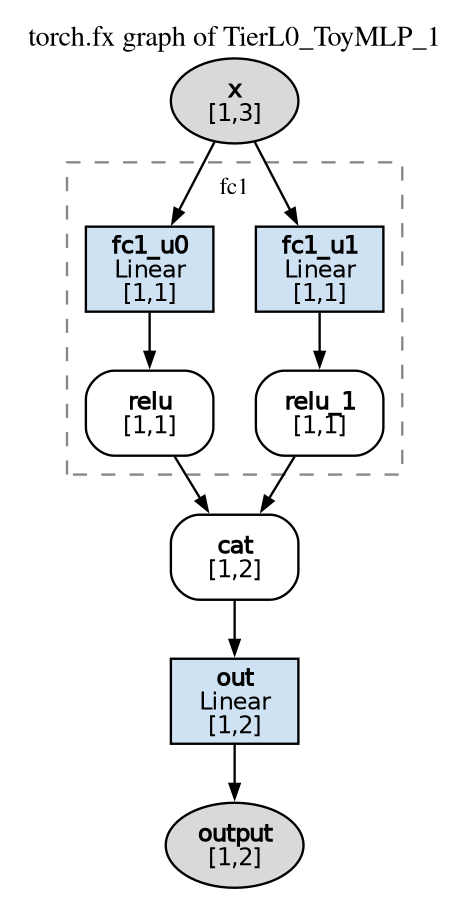
\includegraphics[width=\linewidth,height=0.40\textheight,keepaspectratio]{figs/intro_L0_0000.png}\\\footnotesize(a) the reference graph\end{minipage}\hspace{1cm}
\begin{minipage}[b]{0.45\linewidth}\centering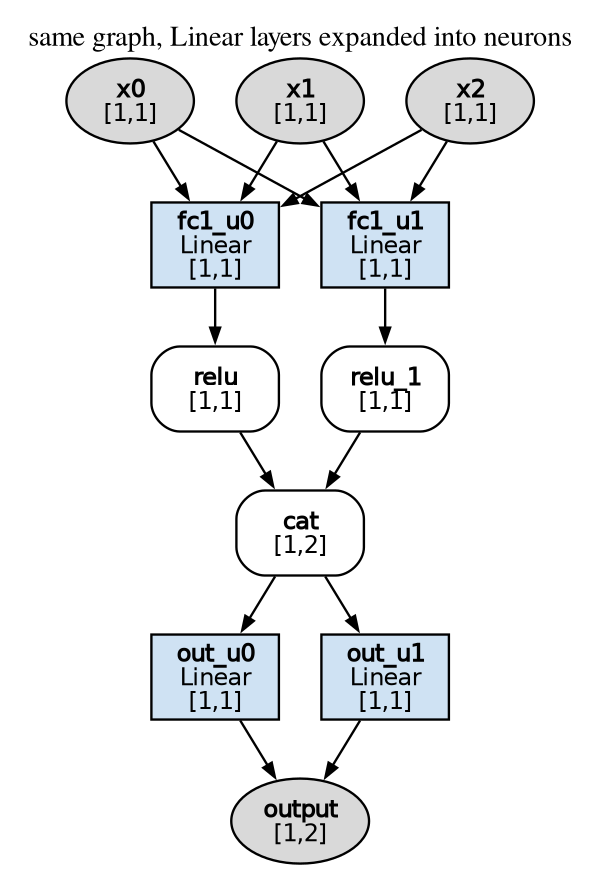
\includegraphics[width=\linewidth,height=0.40\textheight,keepaspectratio]{figs/intro_L0_0000_neurons.png}\\\footnotesize(b) display option: small \texttt{Linear} layers drawn as neurons\end{minipage}
\caption{The torch.fx graph of the module above, drawn by our visualiser. Blue boxes are layers (\texttt{call\_module}:
name, class, output shape); white rounded boxes are functions; grey ellipses are the input and output. The dashed box is
a ``hierarchy cluster'': layers that share a name prefix (\texttt{fc1\_}).}\label{fig:intro}
\end{figure}

\paragraph{What the model has to output.} The LLM writes the same graph in a compact JSON format we call
\textbf{CG-JSON} (``compact graph JSON''): a list of nodes (\texttt{name}, \texttt{op}, \texttt{kind}, \texttt{shape})
and a list of edges as index pairs into that list. For the example above the full answer is:
\lstinputlisting[style=plain]{code/intro_cg.json}

\paragraph{Why this is a good test of an LLM.} The model must (i) find which layers are actually used and in what order,
(ii) follow variables through the code to get the wiring right, including long \emph{skip connections} and merges,
(iii) know PyTorch naming conventions (\texttt{relu}, \texttt{relu\_1}, \dots), and (iv) do arithmetic on tensor shapes.
Because \texttt{torch.fx} gives the exact answer, everything can be scored automatically. \texttt{torch.fx} is therefore
both the \emph{label source} and the \emph{upper bound} (it scores 100\% on every traceable set by construction). The
LLM is interesting where tracing is impossible (data-dependent \texttt{if}s, incomplete code) and as a study of how well
LLMs reason about graph structure.

%==========================================================================================================
\section{The data}\label{sec:data}

\subsection{The given dataset (5,000 samples)}
Our teammate built the dataset: 5{,}000 JSON records, each with \texttt{source\_code} (exactly one \texttt{nn.Module}
class) and its \texttt{target\_graph} from \texttt{torch.fx}. It is organised in five \emph{complexity tiers}:

\begin{center}\small
\begin{tabular}{lp{8.0cm}cc}\toprule
Tier & What the architectures look like & nodes (min/med/max) & distinct topologies \\\midrule
L0 & toy MLP where every hidden unit is its own \texttt{Linear(k,1)} (``neurons'') & 8 / 10 / 14 & 6 \\
L1 & linear chain of conv / batch-norm / activation / dropout & 6 / 15 / 26 & 21 \\
L2 & residual blocks (skip connection, optional projection) & 9 / 17 / 26 & 14 \\
L3 & multiple parallel branches merged by \texttt{torch.cat} & 8 / 12 / 20 & 12 \\
L4 & nested: stem $\to$ 2 paths $\to$ concat $\to$ merge $\to$ residual add $\to$ head & 15 / 17 / 19 & 4 \\\bottomrule
\end{tabular}
\end{center}

There are 1{,}250 \emph{families} (one base architecture each), and every family appears in four variants with an
\emph{identical} graph: the original, the forward argument renamed (e.g.\ \texttt{feat\_map}), dead code inserted
(\texttt{self.unused\_op\_K = nn.Identity()} that is called but never used), and all three changes plus a shuffled
\texttt{\_\_init\_\_}. The official split is 4{,}000 train / 1{,}000 test, separated by family. Inputs are always batch 1
and $16\times16$ images, so shapes are predictable from the code (Figure~\ref{fig:sizes}).

\begin{figure}[H]\centering
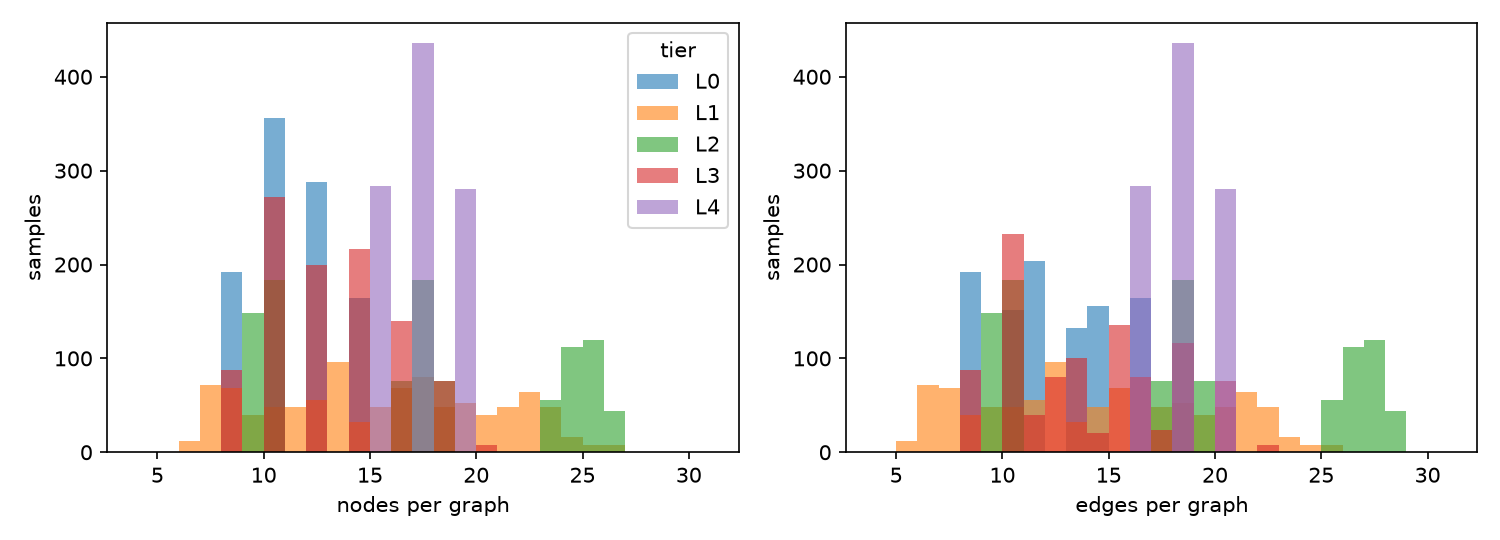
\includegraphics[width=0.85\linewidth]{figs/dataset_sizes.png}
\caption{Graph sizes per tier (all 5,000 samples).}\label{fig:sizes}
\end{figure}

\begin{warnbox}{Three weaknesses of the dataset we had to design around}
\begin{enumerate}[leftmargin=*]
\item \textbf{Very few topologies.} Ignoring names, there are only \textbf{54 distinct graph structures} in all 5{,}000
samples (L4 has 4), and every structure in the official test also occurs in training. The official test therefore
measures ``new code, \emph{seen} topology''. A model could score highly by memorising templates.
\item \textbf{Class names leak the tier} (\texttt{TierL2\_Residual\_17}).
\item \textbf{Everything is flat}: no nested submodule classes, no \texttt{ModuleList}, no pooling in most tiers.
\end{enumerate}
\end{warnbox}

\subsection{The evaluation sets we added}
\begin{itemize}[leftmargin=*]
\item \textbf{test} (1{,}000): the official test, unchanged. 200 of its samples happen to have a structure we held out
(below), so we can split it into ``seen'' and ``held-out'' topologies.
\item \textbf{novel\_topo} (564): before any training we removed 11 of the topology classes (1--4 per tier, chosen with a
fixed random seed, never the largest) from the training data entirely. \texttt{novel\_topo} contains official-train
samples with those structures, so the fine-tuned models have never seen these graph shapes.
\item \textbf{test\_anon} (1{,}000): the official test with every class renamed to \texttt{Net}.
\item \textbf{OOD-1} (40): hand-written ``out-of-distribution'' modules in 10 categories: MLPs with LayerNorm/GELU,
VGG-style with pooling, nested ResNet blocks (submodule classes), bottlenecks with \texttt{F.relu}, Inception branches,
U-Net with up-sampling, DenseNet concatenations, Squeeze-and-Excitation (tensor methods + broadcasting multiply),
two-input models, and \texttt{ModuleList}/\texttt{Sequential} loops.
\item \textbf{OOD-2} (21): written \emph{after} the synthetic generator (Section~\ref{sec:synth}) was frozen, using
constructs that occur in neither the dataset nor the generator: functional pooling, \texttt{view}/\texttt{reshape}/
\texttt{permute}, attention with \texttt{matmul}+\texttt{softmax}, transposed convolutions, GroupNorm/PReLU/ELU/Hardswish,
\texttt{torch.stack}, scalar arithmetic. It is the most honest generalisation test we have.
\item \textbf{untraceable} (6): modules \texttt{torch.fx} cannot trace (data-dependent \texttt{if}/\texttt{while},
\texttt{assert}, \texttt{int(x.shape)}): no reference, used only to show what models do.
\item \textbf{val} (160) and \textbf{test\_mini} (100, stratified) for training sanity checks and expensive experiments.
\end{itemize}
Fine-tuning used \textbf{train\_ft} = 3{,}068 samples (official train minus the held-out structures minus val).
Nothing from any evaluation set was ever used for training, prompts or model selection.

\subsection{Synthetic training data (the ``aug'' experiment)}\label{sec:synth}
To attack the ``54 topologies'' problem we wrote a generator (\texttt{scripts/gen\_synthetic.py}) that composes random
architectures from general PyTorch building blocks (residual blocks, branch-concat, pooling, U-Net skips, dense
concatenations, gating, nested block classes, \texttt{Sequential}, \texttt{ModuleList} loops, two-input fusion, MLPs),
with random (sometimes deliberately misleading) attribute names. Every module is labelled by the same oracle and kept only
if the validator accepts the gold graph. We generated 3{,}200 modules (2{,}090 distinct structures); 2{,}809 fit the token
budget and were added to train\_ft. \textbf{Leakage guard:} any generated module whose structure equals a
\texttt{novel\_topo} or OOD-1 structure was discarded (264 were); a separate audit found zero overlap.

%==========================================================================================================
\section{How the system works (and where the code is)}\label{sec:system}

\begin{figure}[H]\centering
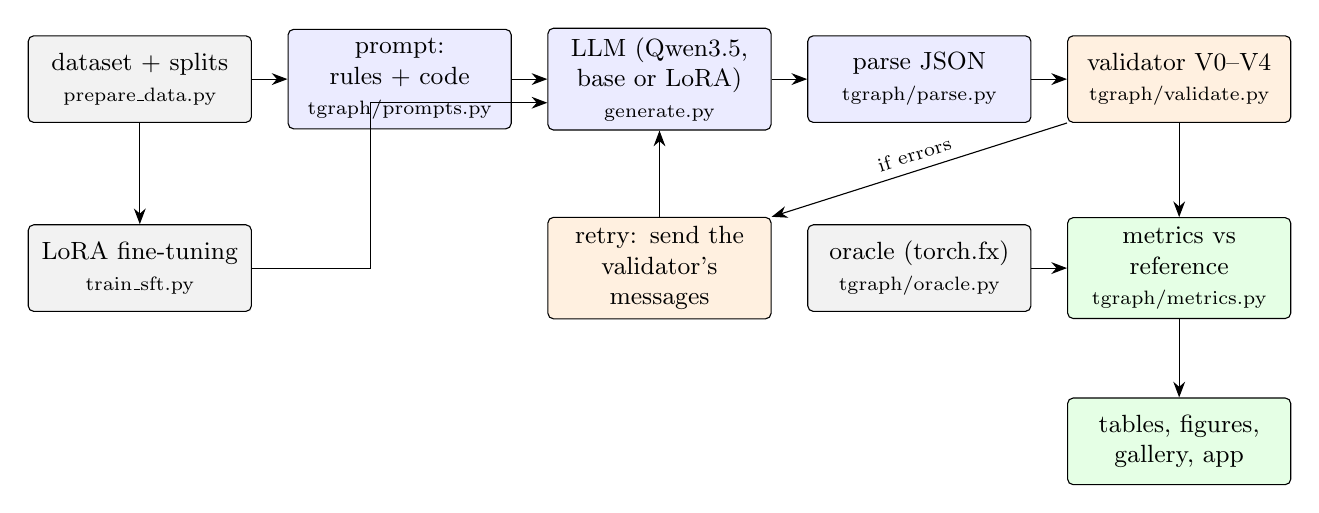
\begin{tikzpicture}[box/.style={draw,rounded corners=2pt,fill=#1,align=center,font=\small,minimum height=11mm,text width=26mm},>={Stealth[length=2mm]}]
\node[box=gray!10]   (data)   at (0,0)     {dataset + splits\\\scriptsize prepare\_data.py};
\node[box=blue!8]    (prompt) at (3.3,0)   {prompt: rules + code\\\scriptsize tgraph/prompts.py};
\node[box=blue!8]    (llm)    at (6.6,0)   {LLM (Qwen3.5,\\base or LoRA)\\\scriptsize generate.py};
\node[box=blue!8]    (parse)  at (9.9,0)   {parse JSON\\\scriptsize tgraph/parse.py};
\node[box=orange!12] (val)    at (13.2,0)  {validator V0--V4\\\scriptsize tgraph/validate.py};
\node[box=gray!10]   (train)  at (0,-2.4)  {LoRA fine-tuning\\\scriptsize train\_sft.py};
\node[box=orange!12] (retry)  at (6.6,-2.4) {retry: send the\\validator's messages};
\node[box=gray!10]   (oracle) at (9.9,-2.4) {oracle (torch.fx)\\\scriptsize tgraph/oracle.py};
\node[box=green!10]  (met)    at (13.2,-2.4) {metrics vs reference\\\scriptsize tgraph/metrics.py};
\node[box=green!10]  (out)    at (13.2,-4.6) {tables, figures,\\gallery, app};
\draw[->] (data) -- (prompt); \draw[->] (prompt) -- (llm); \draw[->] (llm) -- (parse); \draw[->] (parse) -- (val);
\draw[->] (data) -- (train); \draw[->] (train.east) -- ++(1.5,0) |- ([yshift=-3mm]llm.west);
\draw[->] (val.south west) -- node[font=\scriptsize,sloped,above]{if errors} (retry.north east);
\draw[->] (retry) -- (llm);
\draw[->] (val) -- (met); \draw[->] (oracle) -- (met); \draw[->] (met) -- (out);
\end{tikzpicture}
\caption{The pipeline. The validator never sees the answer, so it can be used at inference time (retry) and in the
app; the oracle is used only for scoring.}\label{fig:pipeline}
\end{figure}

\begin{center}\small
\begin{tabular}{p{4.1cm}p{11.3cm}}\toprule
File & What it does \\\midrule
\texttt{tgraph/oracle.py} & runs \texttt{torch.fx}: trace, remove dead code, propagate shapes. Reproduces all 5{,}000 labels byte-for-byte (a test checks this). A sandboxed version runs user code in a separate process with a 20\,s limit. \\
\texttt{tgraph/schema.py} & converts between the dataset format and CG-JSON; the JSON schema used for constrained decoding. \\
\texttt{tgraph/prompts.py} & the system prompt (8 rules: node order, naming, \texttt{call\_module} vs \texttt{call\_function}, dead code, shape convention, edge format), chat rendering, few-shot and retry messages. \\
\texttt{tgraph/parse.py} & extracts JSON from raw model text (removes \texttt{<think>} blocks and code fences, finds the first balanced \texttt{\{\dots\}}, repairs truncated JSON). \\
\texttt{tgraph/codeinfo.py} & reads the source with Python's \texttt{ast} (never executes it): which layers \texttt{\_\_init\_\_} declares, with which arguments, and which of them actually reach the \texttt{return} (a backward ``liveness'' pass). \\
\texttt{tgraph/validate.py} & the 5-level checker (below). \\
\raggedright \texttt{tgraph/align.py}, \texttt{metrics.py}, \texttt{properties.py}, \texttt{failures.py} & node matching, all metrics, topological properties, failure labels. \\
\texttt{tgraph/visualize.py} & Graphviz drawings: single graph, side-by-side, colour-coded diff, neuron expansion; matplotlib fallback. \\
\texttt{scripts/} & \texttt{prepare\_data}, \texttt{build\_ood}, \texttt{gen\_synthetic}, \texttt{train\_sft}, \texttt{merge\_lora}, \texttt{generate}, \texttt{run\_eval}, \texttt{aggregate}, \texttt{plots}, \texttt{gallery}, \dots \\
\texttt{app/} & Gradio demo: paste code $\to$ predicted graph, reference, diff, metrics, validity report. \\
\texttt{configs/}\allowbreak\texttt{experiments.yaml} & every inference configuration (model, prompt mode, decoding, eval sets). \\\bottomrule
\end{tabular}
\end{center}

\subsection{The validator: checking a graph without knowing the answer}
\begin{center}\small
\begin{tabular}{lp{12.5cm}}\toprule
Level & Checks \\\midrule
V0 parse & the output is JSON and follows the schema \\
V1 structure & unique names; edges point to existing nodes; no self-loops/duplicates; one input, one output at the end; no cycles; nodes listed in execution order; every node reachable from the input and leading to the output \\
V2 arity & \texttt{add}/\texttt{mul} need two tensor inputs, \texttt{cat} at least two, a \texttt{Conv2d} exactly one, \dots \\
V3 code consistency & every \texttt{call\_module} node is a layer declared in \texttt{\_\_init\_\_} (otherwise ``hallucinated''), with the declared class; every used layer appears as often as it is called; dead layers do not appear \\
V4 shapes & e.g.\ a \texttt{Conv2d}'s channel count equals its \texttt{out\_channels}; activations keep the shape; \texttt{add} inputs broadcast; \texttt{cat} sums channels; the input shape follows the convention \\\bottomrule
\end{tabular}
\end{center}
A graph is \textbf{fully valid} if it passes V0--V4. The validator has zero false alarms on all 5{,}000 gold graphs and on
all 61 OOD gold graphs, and catches every synthetic corruption in the tests. Its messages are short English sentences
(e.g.\ \texttt{node 15 'add' has 1 input; 'add' of two tensors needs 2 (missing skip edge?)}), which is what makes
\emph{verify-and-retry} possible: failing graphs are sent back to the model together with these messages.

\subsection{Metrics: how close is a prediction to the reference?}
\begin{itemize}[leftmargin=*]
\item \textbf{Node / edge F1}: nodes are matched by name; an edge is correct if the same named pair is connected.
\item \textbf{Exact match}: same nodes (name, op, kind) and same edge set. \textbf{Isomorphic}: same graph up to renaming
(only structure and kinds count).
\item \textbf{Graph similarity} $=1-$ normalised edit distance (how many nodes/edges must change). We validated this
cheap distance against the true graph edit distance on 1{,}378 pairs: Spearman correlation \textbf{0.998}
(Figure~\ref{fig:F8}).
\item \textbf{Property preservation (PPS)}: share of 14 topological properties that match (depth, width, number of
branches/merges/skip edges/paths, \dots). \textbf{Shape accuracy}: share of matched nodes with the right shape.
\item Every number comes with a bootstrap 95\% confidence interval; results are sliced by tier, size, augmentation,
seen/held-out topology and OOD category.
\end{itemize}

\subsection{Models, fine-tuning and inference}
\begin{itemize}[leftmargin=*]
\item \textbf{Models.} Qwen3.5-2B and -9B (the 9B was already on the cluster), Qwen3.5-27B in FP8 as the ``ceiling'',
Qwen2.5-Coder-7B as an older code-specialised baseline. Qwen3.5 mixes normal attention with ``Gated DeltaNet''
linear-attention layers, which needs special GPU kernels (\texttt{flash-linear-attention}).
\item \textbf{Prompting.} Zero-shot (rules + code) and 3-shot (plus three solved training examples).
\item \textbf{Fine-tuning} (LoRA, bf16, 2 epochs): small trainable matrices added to every attention, MLP and
linear-attention projection; the loss is computed only on the answer tokens. Training is short: 2B 0.5\,h, 9B 1.5\,h
(3\,h with synthetic data) on one NVIDIA L40S. Training and inference use byte-identical prompts.
\item \textbf{Inference} with vLLM, greedy decoding. \emph{Constrained decoding} forces the output to match the JSON
schema. \emph{Verify-and-retry}: up to 2 extra rounds with the validator's messages. \emph{Self-consistency}: 5 samples,
the validator picks. \emph{Thinking mode}: Qwen3.5 reasons in a \texttt{<think>} block before answering.
\end{itemize}

%==========================================================================================================
\section{The journey: what we did, what broke, what we changed}\label{sec:journey}

\noindent\textbf{1. Setting up without disturbing the other project.} The cluster account also runs a separate research
project whose final evaluation depends on bit-exact caches. Everything here (two new Python environments, model
downloads, Hugging Face / Triton / vLLM / pip caches) lives under \texttt{\textasciitilde/IE643\_Project}. One leak was
found and fixed: vLLM and flashinfer wrote caches into the shared home folder; they were moved and redirected.

\noindent\textbf{2. Getting the software stack to run} took several rounds:
\begin{itemize}[leftmargin=*]
\item The GPU driver supports CUDA 12.8, but the newest vLLM needs a newer PyTorch with no CUDA-12.8 build $\to$ vLLM
0.26 with a CUDA 12.9 build (CUDA minor-version compatibility, verified on the GPU).
\item \texttt{import vllm} failed three times in a row: a video-decoding library built for CUDA 13, then missing FFmpeg
libraries, then a C++ runtime that was too old. Each was fixed inside our own environment.
\item vLLM's default sampler tries to compile CUDA code at run time, and the cluster has no CUDA compiler $\to$ switched
to vLLM's PyTorch sampler.
\item transformers picks the fast Triton kernels for Qwen3.5 even on a CPU, where Triton crashes $\to$ a switch that
disables them on CPU-only runs. Even then, \textbf{training Qwen3.5 on a CPU was hopeless} (one step of 870 tokens did
not finish in 25 minutes), so all training happened on GPUs.
\item The installed library versions had renamed training arguments; the 27B model needed fewer parallel sequences to
fit next to its weights.
\end{itemize}

\noindent\textbf{3. Verifying before spending GPU time.} Before the real runs: all 28 unit tests (oracle = labels on all
5{,}000 samples, validator silent on all gold graphs, metrics behave on corruptions), a merge check (merged weights
reproduce the adapter within bf16 rounding), a dry run of the whole evaluation chain on fake predictions, a GPU smoke test
(9B: 12\,s per step, 21\,GB), and a token-level check that the model is trained on exactly the answer plus one end token.

\noindent\textbf{4. The prompt bug.} The first real zero-shot run scored \textbf{0\%} valid: 957 of 1{,}000 answers
failed only because the spec's prompt never said that the input node's \texttt{kind} is \texttt{"placeholder"} (the models
wrote \texttt{"input"}). We clarified the rule, asked for compact one-line JSON (12\% of answers had run out of tokens
while pretty-printing), rebuilt the training files and restarted every job. Zero-shot rose to 19.9\%; the remaining
zero-shot failures are genuine (e.g.\ the runaway loop in Example 6).

\noindent\textbf{5. Thinking mode needed room.} With the spec's 8{,}192-token budget, 97\% of thinking answers were
still reasoning when cut off. With 30{,}000 tokens most finished, with excellent topology but missing shapes; forcing
the JSON format \emph{after} the reasoning (``think-then-constrain'') fixed the format. Thinking costs 17--22k tokens per
graph (about 20$\times$ a normal answer).

\noindent\textbf{6. The night of experiments.} After the planned runs, the weak spot was clear: models fine-tuned on 54
templates fail on new code. We added the synthetic-data arm, the 27B ceiling, combinations of retry and
self-consistency, and OOD-2. Every change is recorded with its reason in \texttt{DECISIONS.md}; the full log is
\texttt{PROJECT\_LOG.md}.

%==========================================================================================================
\section{Results}\label{sec:results}

\subsection{The main table}
\begin{table}[H]\centering\small
\begin{tabular}{lccccc}\toprule
& \multicolumn{5}{c}{\textbf{fully valid, \%} \quad(exact match \% in brackets)} \\
Configuration & test (1{,}000) & test\_anon & novel\_topo (564) & OOD-1 (40) & OOD-2 (21) \\\midrule
2B 3-shot & 1.1 (6.5) & -- & 1.1 (3.2) & 0.0 (0.0) & 0.0 (4.8) \\
Coder-7B 3-shot & 15.4 (21.7) & -- & 6.9 (19.1) & 10.0 (5.0) & 47.6 (33.3) \\
9B zero-shot & 19.9 (20.3) & -- & 10.3 (14.0) & 12.5 (5.0) & 38.1 (28.6) \\
9B 3-shot & 54.9 (57.1) & 47.0 (50.4) & 32.3 (33.9) & 27.5 (30.0) & 47.6 (38.1) \\
9B 3-shot + retry & -- & -- & -- & 45.0 (40.0) & 71.4 (66.7) \\
27B zero-shot + retry & -- & -- & 87.9 (90.8) & \textbf{100} (87.5) & 90.5 (85.7) \\
27B 3-shot & 91.0 (97.9) & -- & 92.4 (99.1) & 80.0 (70.0) & \textbf{95.2} (90.5) \\\midrule
2B fine-tuned & 93.3 (93.7) & 93.4 & 64.4 (64.5) & 5.0 (2.5) & 28.6 (19.0) \\
2B FT + synthetic & \textbf{100} (100) & 99.8 & \textbf{100} (100) & 72.5 (70.0) & 71.4 (52.4) \\
9B fine-tuned & 99.7 (99.7) & 99.6 & \textbf{100} (100) & 47.5 (30.0) & 85.7 (71.4) \\
9B fine-tuned + retry & 99.7 (99.7) & -- & \textbf{100} (100) & 67.5 (45.0) & 90.5 (76.2) \\
9B FT + synthetic & \textbf{100} (100) & \textbf{100} & \textbf{100} (100) & 95.0 (97.5) & 76.2 (76.2) \\
9B FT + synthetic + retry & \textbf{100} (100) & -- & \textbf{100} (100) & 97.5 (97.5) & 90.5 (76.2) \\\bottomrule
\end{tabular}
\caption{Headline results (all constrained decoding, greedy). ``--'' = not run. ``Fully valid'' = passes all
validator levels; ``exact'' = identical nodes and edges (ignores shapes, so it can exceed validity). On the small OOD
sets one module is 2.5 (OOD-1) or 4.8 (OOD-2) percentage points.}\label{tab:main}
\end{table}

\begin{figure}[H]\centering
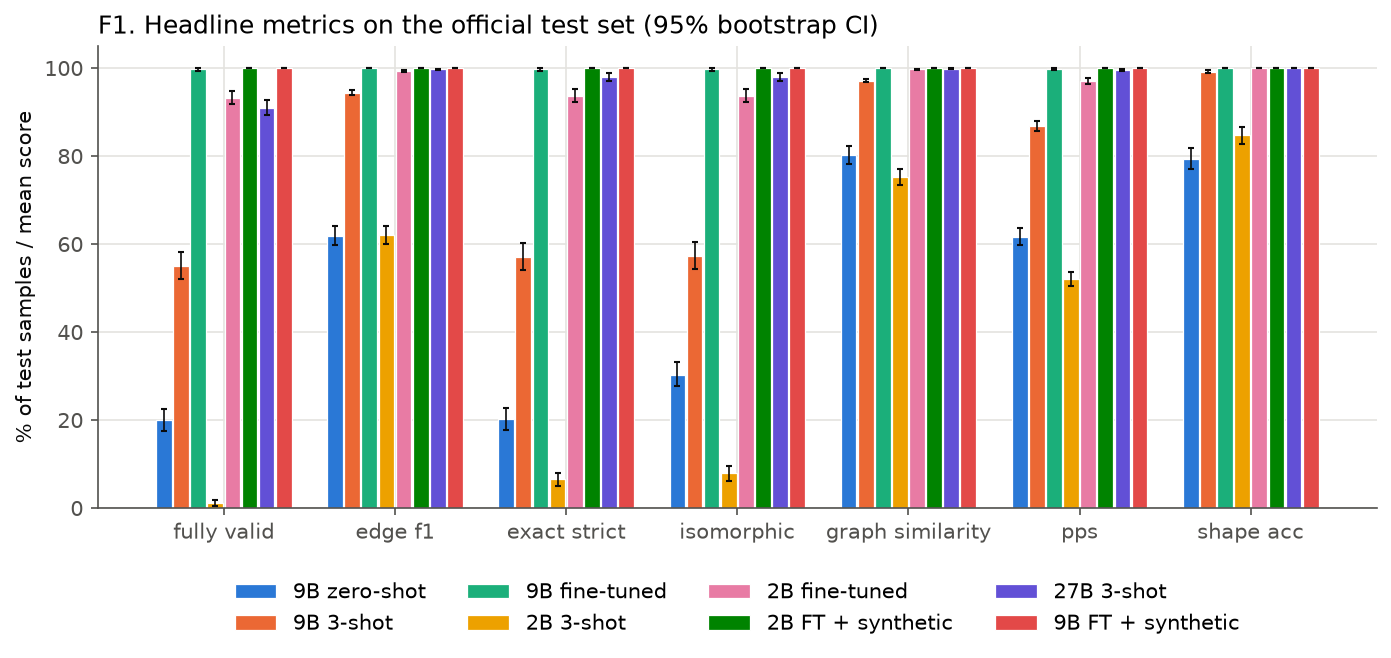
\includegraphics[width=0.95\linewidth]{figs/F1_headline.png}
\caption{Headline metrics on the official test with 95\% bootstrap confidence intervals (F1).}\label{fig:F1}
\end{figure}

\subsection{Complexity: which architectures are hard?}
\begin{figure}[H]\centering
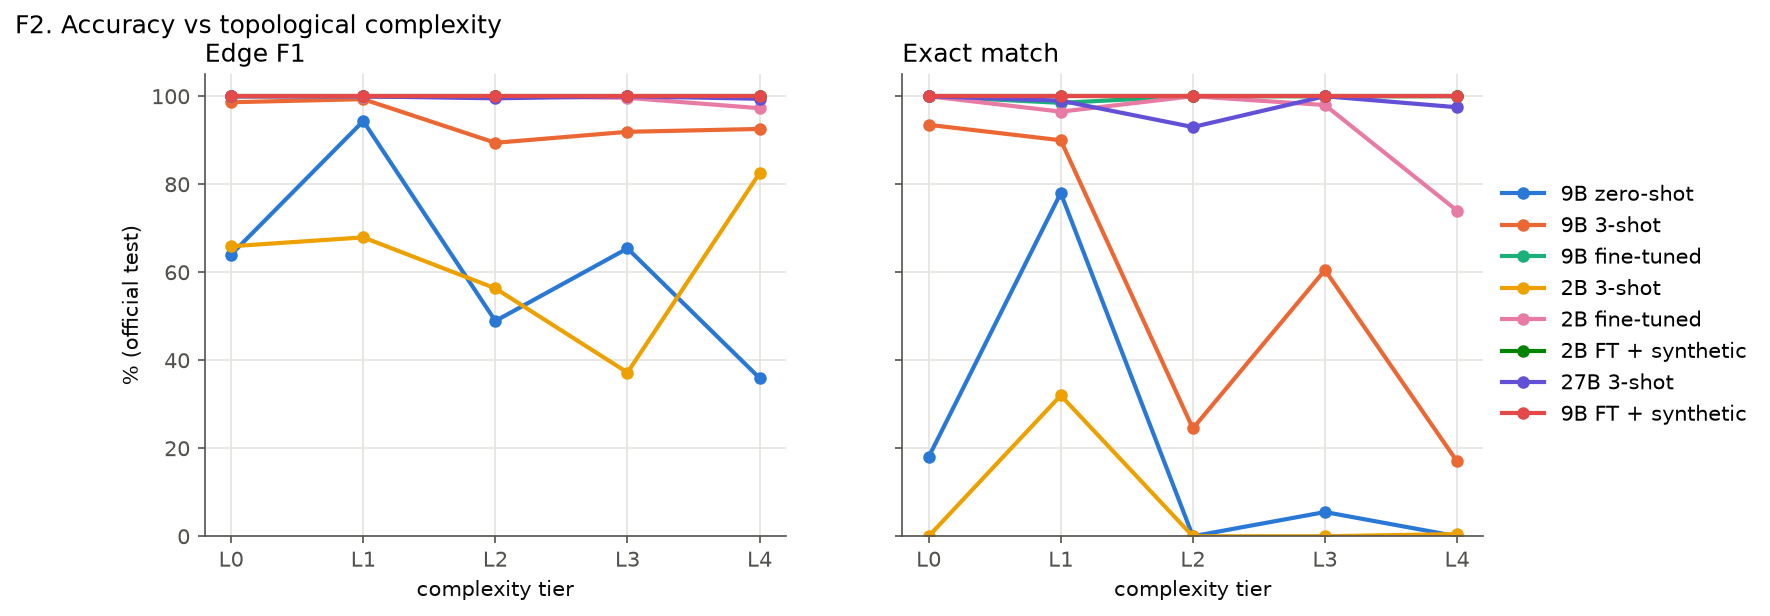
\includegraphics[width=0.95\linewidth]{figs/F2_by_tier.png}
\caption{Edge F1 and exact match by tier (official test). For the prompted models, L2 (residual) and L4 (nested) are the
hard tiers: 9B 3-shot exact match is 93.5\% on L0 but 24.5\% on L2 and 17.0\% on L4. The long skip edge into an
\texttt{add} is the typical miss. Fine-tuned models are flat at $\approx$100\%.}\label{fig:F2}
\end{figure}

\subsection{Memorisation versus generalisation}
\begin{figure}[H]\centering
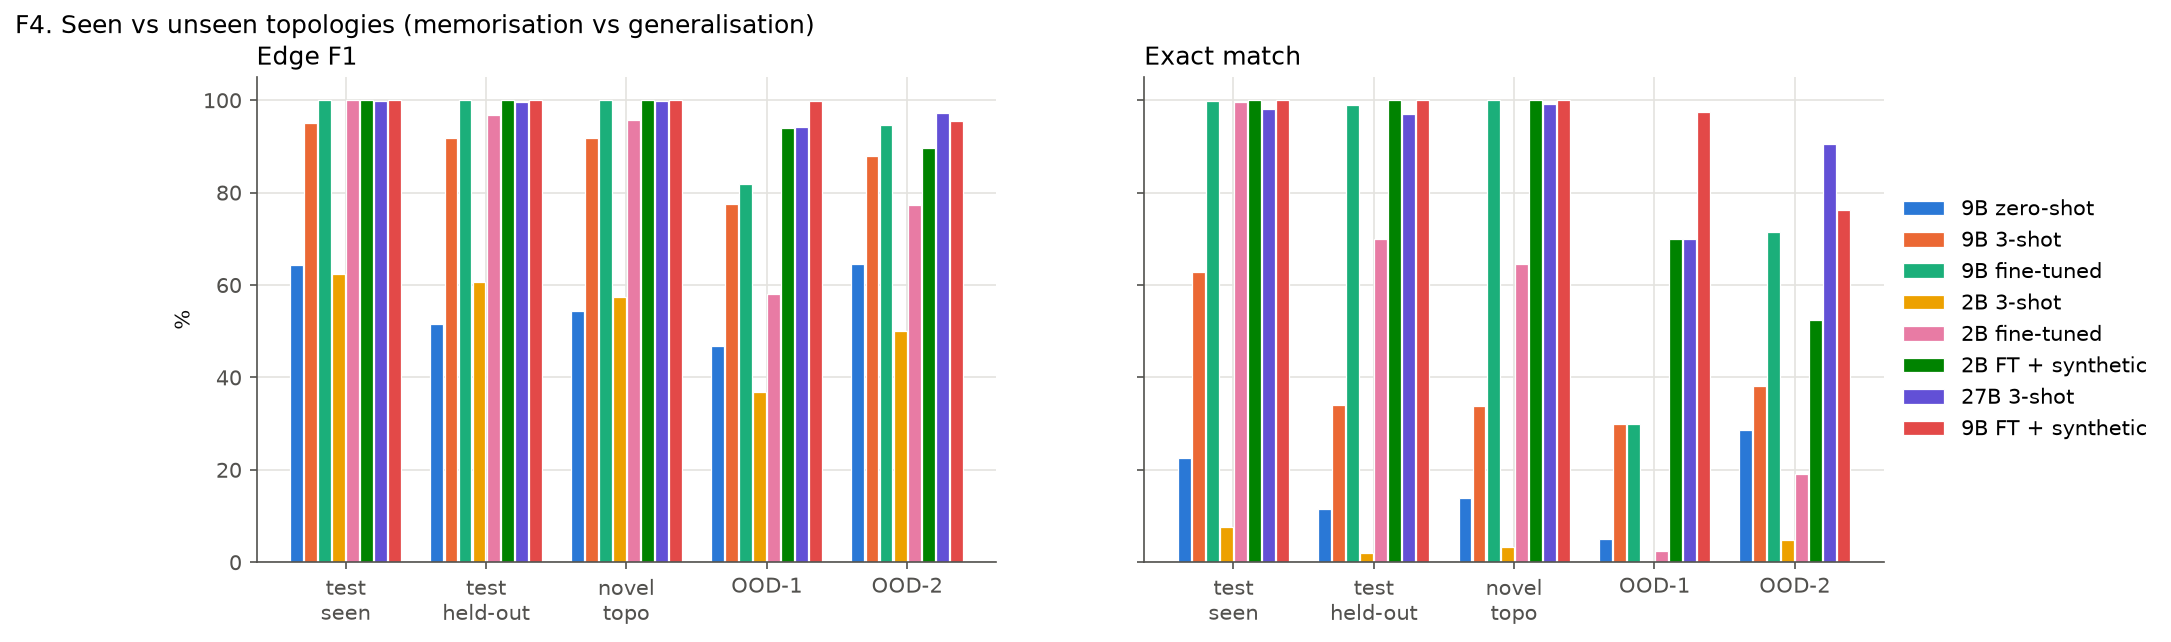
\includegraphics[width=\linewidth]{figs/F4_seen_vs_unseen.png}
\caption{From left to right the test sets move further from the training data: test samples with a seen topology,
test samples with a held-out topology, the novel\_topo set, OOD-1 and OOD-2. Plain fine-tuning (light green, pink) is
near-perfect until OOD-1, where it collapses; the synthetic-data models (dark green, red) and the 27B (purple) hold up.}\label{fig:F4}
\end{figure}
Inside the test set, the fine-tuned 2B scores 99.3\% on seen topologies but 69.5\% on held-out ones, and \textbf{0\% on
the held-out L4 topology}; the fine-tuned 9B scores 99.0\% on held-out topologies including 100\% on that L4 structure
(Example 5). Scale decides whether a fine-tuned model memorises templates or learns the rules.

\subsection{Robustness, validity and self-correction}
\begin{figure}[H]\centering
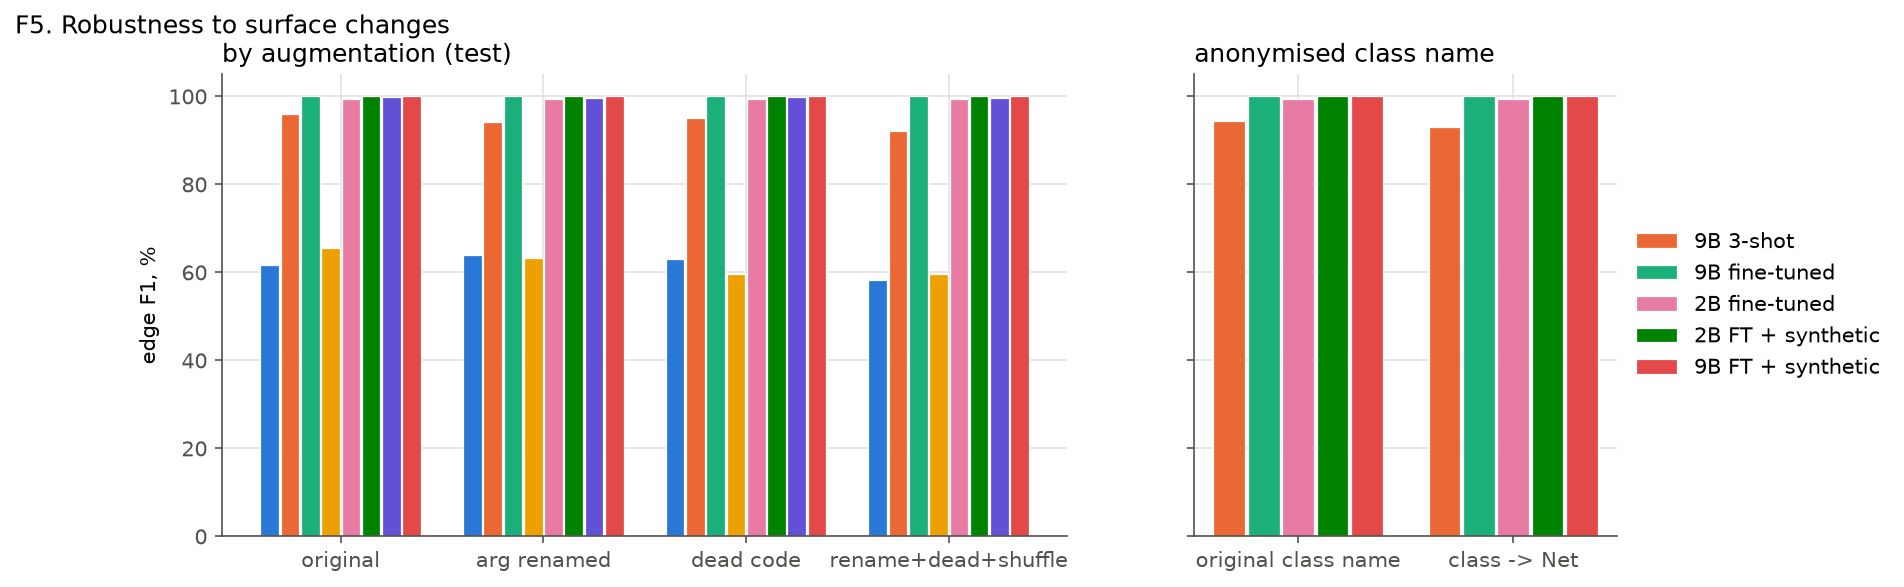
\includegraphics[width=0.92\linewidth]{figs/F5_robustness.png}
\caption{Robustness to renaming, dead code and anonymised class names (F5). The 9B 3-shot model drops from 54.9\% to
47.0\% valid when class names are replaced by \texttt{Net} (it uses the tier hint in the name); fine-tuned models do not
care (93.3/93.4\% for 2B, 99.7/99.6\% for 9B).}\label{fig:F5}
\end{figure}
\begin{figure}[H]\centering
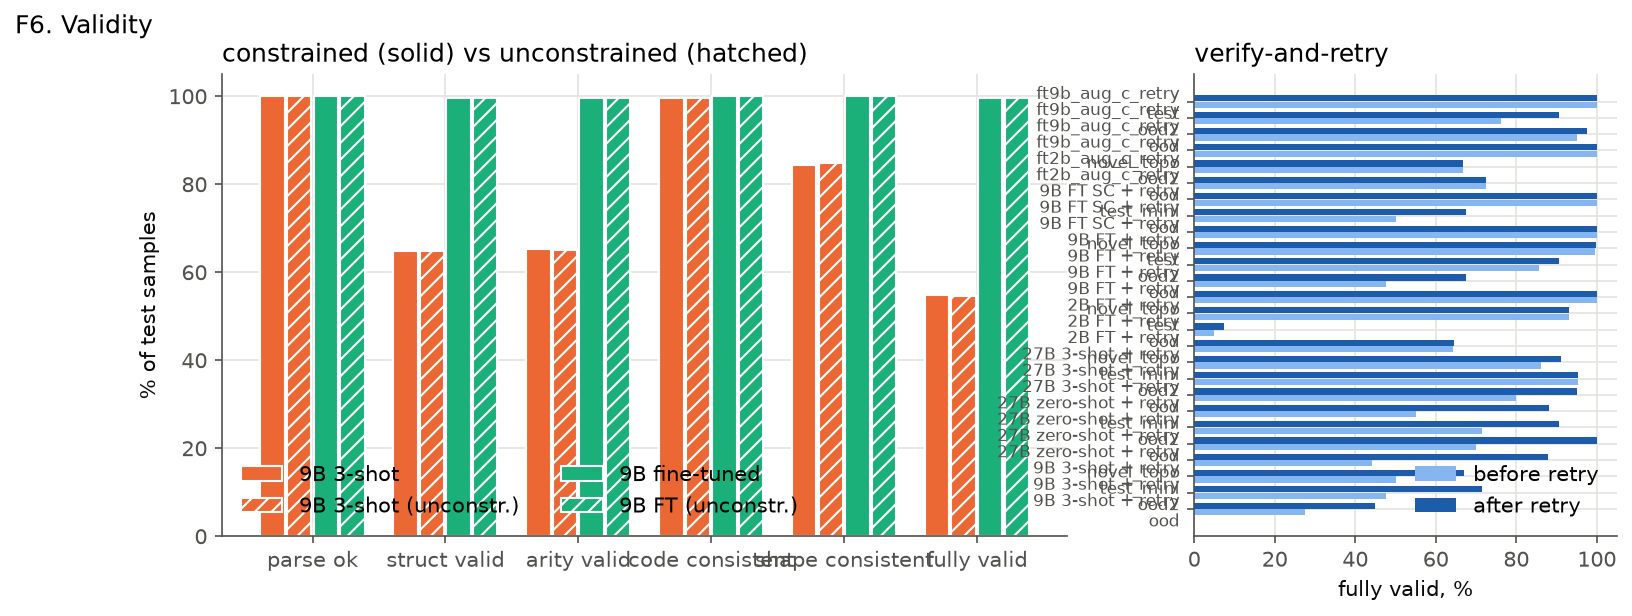
\includegraphics[width=0.92\linewidth]{figs/F6_validity.png}
\caption{Left: validity levels with (solid) and without (hatched) constrained decoding. Constraining the JSON hardly
matters (9B 3-shot: 54.9\% vs 54.6\%; fine-tuned 9B: identical), because these models already write valid JSON; the
errors are in the content. Right: verify-and-retry before and after (F6).}\label{fig:F6}
\end{figure}

\begin{table}[H]\centering\small
\begin{tabular}{llccc}\toprule
Model & set & valid before retry & valid after retry & mean rounds \\\midrule
27B zero-shot & OOD-1 & 70.0 & \textbf{100.0} & 0.33 \\
27B zero-shot & novel\_topo & 44.1 & 87.9 & 0.79 \\
9B fine-tuned & OOD-1 & 47.5 & 67.5 & 0.93 \\
9B FT + synthetic & OOD-2 & 76.2 & 90.5 & 0.38 \\
9B 3-shot & OOD-1 & 27.5 & 45.0 & 1.28 \\
2B fine-tuned & OOD-1 & 5.0 & 7.5 & 1.90 \\
2B FT + synthetic & OOD-1 & 72.5 & 72.5 & 0.55 \\\bottomrule
\end{tabular}
\caption{Verify-and-retry uses only the validator, never the answer. It helps the 9B and 27B models a lot and the
2B models not at all: small models cannot act on the feedback.}\label{tab:retry}
\end{table}

\subsection{Failure modes, properties, metric check, training}
\begin{figure}[H]\centering
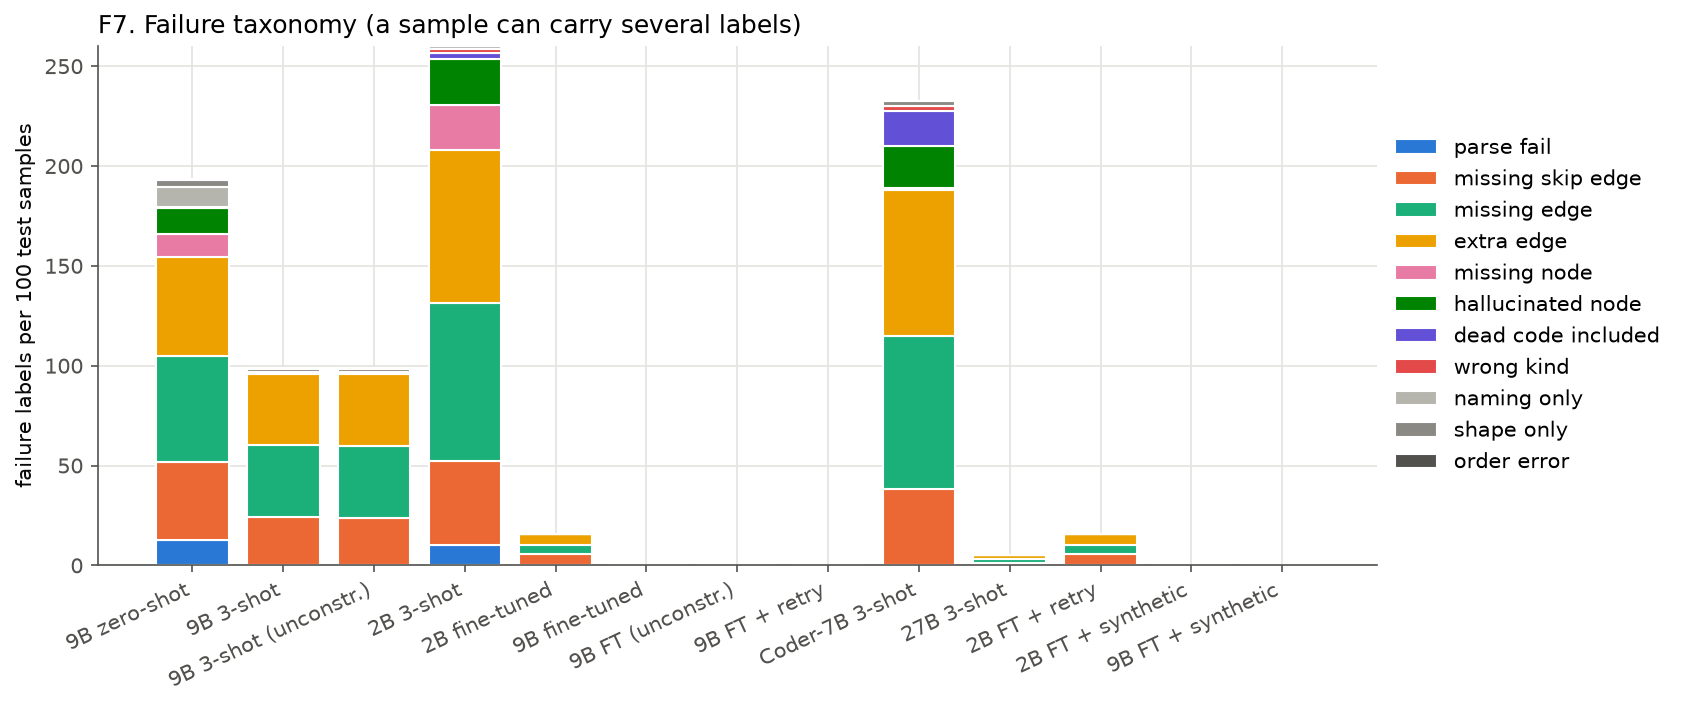
\includegraphics[width=0.92\linewidth]{figs/F7_failures.png}
\caption{Failure labels per 100 test samples (a sample can have several). Prompted models mostly miss edges (ordinary
and skip edges) and invent extra ones; parse failures are the zero-shot runaway loops.}\label{fig:F7}
\end{figure}
\begin{figure}[H]\centering
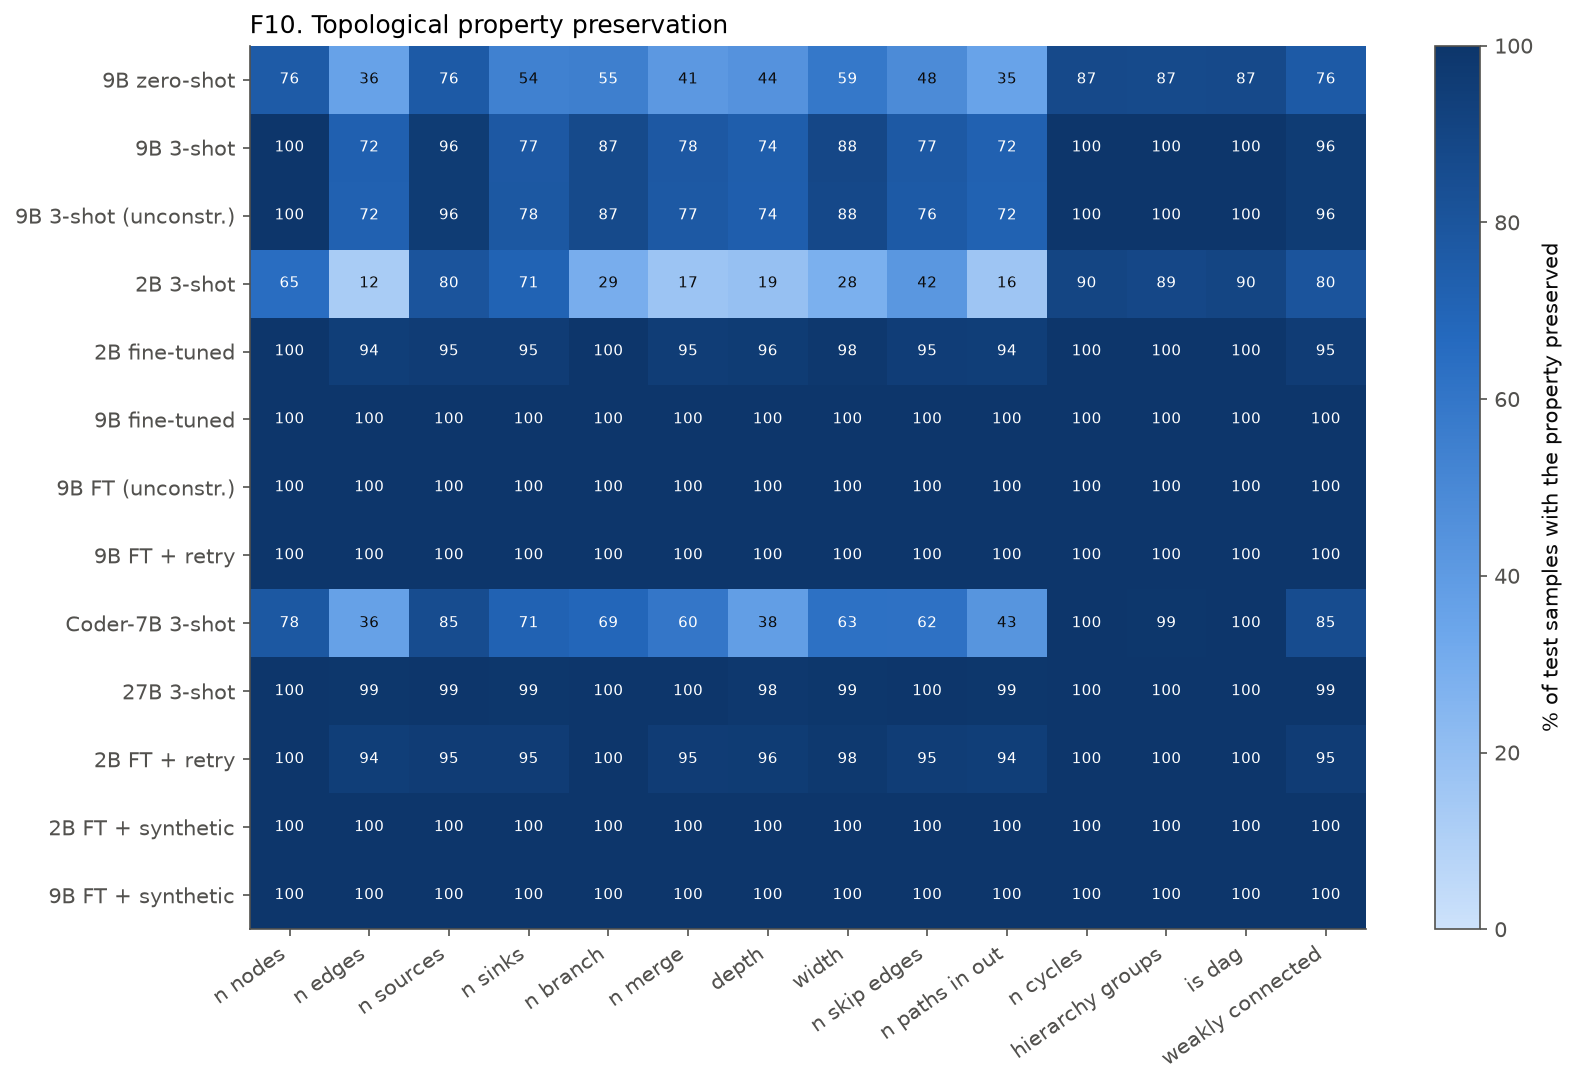
\includegraphics[width=0.95\linewidth]{figs/F10_properties.png}
\caption{How often each topological property of the reference is preserved (official test).}\label{fig:F10}
\end{figure}
\begin{figure}[H]\centering
\begin{minipage}{0.44\linewidth}\centering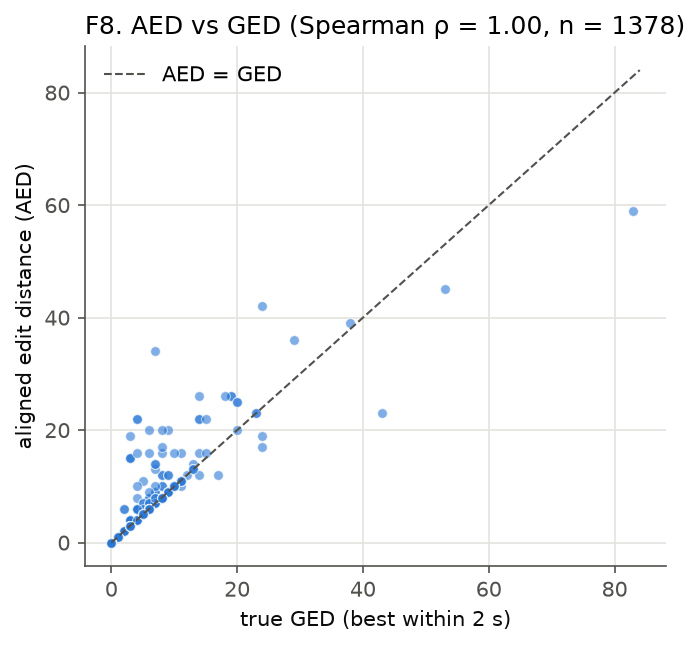
\includegraphics[width=\linewidth]{figs/F8_aed_vs_ged.png}\end{minipage}\hfill
\begin{minipage}{0.54\linewidth}\centering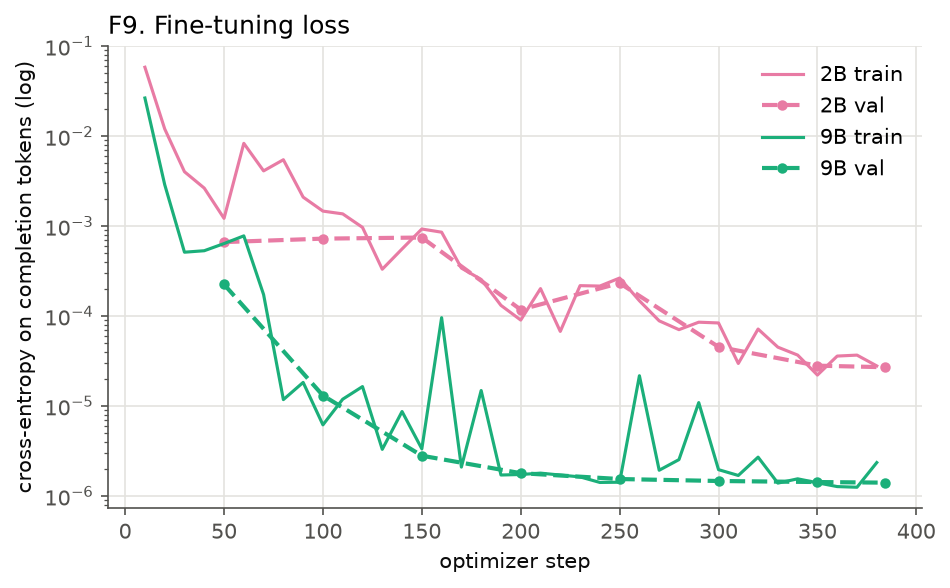
\includegraphics[width=\linewidth]{figs/F9_loss.png}\end{minipage}
\caption{Left (F8): our fast aligned edit distance vs the true graph edit distance (Spearman 0.998; it is never
below the true value). Right (F9): training and validation loss of the 2B and 9B fine-tunes (log scale); both reach
losses near zero, as expected on templated data.}\label{fig:F8}
\end{figure}

%==========================================================================================================
\section{Twelve worked examples, from code to graph}\label{sec:examples}
Each example shows the code, a small results table, and drawings: the reference (from \texttt{torch.fx}) and one or
two model predictions, usually as a \textbf{diff} against the reference. In a diff, black edges are correct,
\textcolor{red}{red dashed} nodes and edges are in the reference but missing from the prediction,
\textcolor{orange}{orange} ones are invented by the model, and red text marks a wrong layer type or shape.
\clearpage
\subsection{Example 1: A neuron-level MLP (tier L0)}\label{sec:ex01}
{\small set: official test \textbullet{} sample: \texttt{L0\_0803} \textbullet{} tier L0 \textbullet{} augmentation: \texttt{aug\_variant\_3} \textbullet{} topology seen in training \textbullet{} 10 nodes}

\lstinputlisting[style=py]{code/ex01.py}
\begin{center}\footnotesize\begin{tabular}{lcccccp{4.6cm}}\toprule
model & valid & edge F1 & exact & shape acc. & tokens & failure labels \\ \midrule
9B zero-shot & no & 0.55 & no & 0.88 & 268 & \raggedright naming only \tabularnewline
9B fine-tuned & yes & 1.00 & yes & 1.00 & 263 & \raggedright -- \tabularnewline
\bottomrule\end{tabular}\end{center}
\textbf{What to look at.} Every hidden unit is its own \texttt{Linear(k,1)} (``neurons'' made explicit). This
sample is an \emph{augmented} variant: the forward argument is renamed (\texttt{inp\_tensor}), a dead layer is inserted
and the \texttt{\_\_init\_\_} order is shuffled. The zero-shot 9B model wires the graph correctly (it is
\emph{isomorphic} to the reference) but names the input after the argument instead of \texttt{x}, picks the wrong input
width ($[1,3]$ instead of $[1,2]$) and therefore gets node and edge \emph{names} wrong: strict edge F1 is only 0.55
although the shape of the graph is right. The fine-tuned 9B reproduces the reference exactly.

\begin{figure}[H]\centering
\begin{minipage}[b]{0.32\linewidth}\centering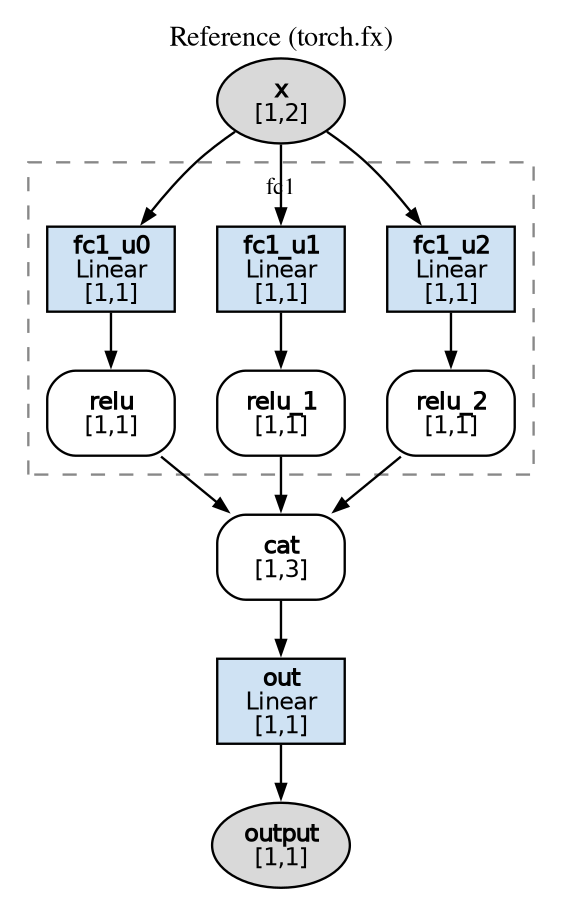
\includegraphics[width=\linewidth,height=0.40\textheight,keepaspectratio]{figs/ex01_ref.png}\\\footnotesize Reference\end{minipage}\hfill
\begin{minipage}[b]{0.32\linewidth}\centering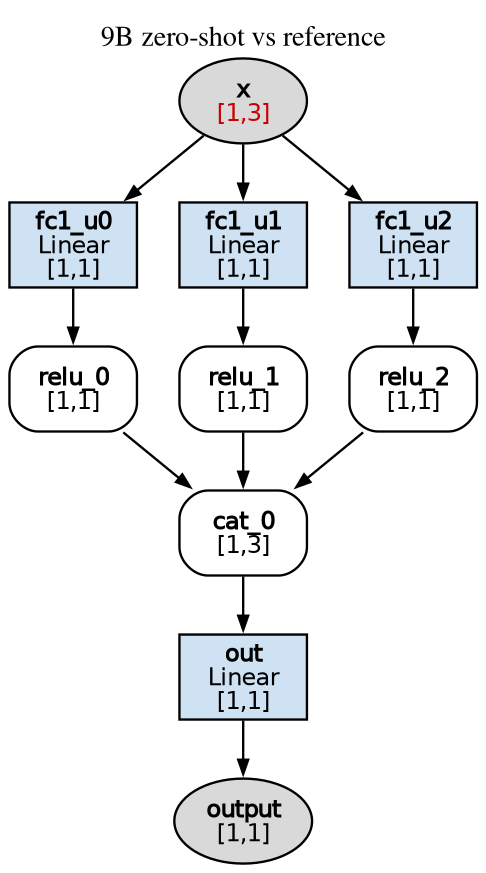
\includegraphics[width=\linewidth,height=0.40\textheight,keepaspectratio]{figs/ex01_base9b_zs_c_diff.png}\\\footnotesize 9B zero-shot vs reference\end{minipage}\hfill
\begin{minipage}[b]{0.32\linewidth}\centering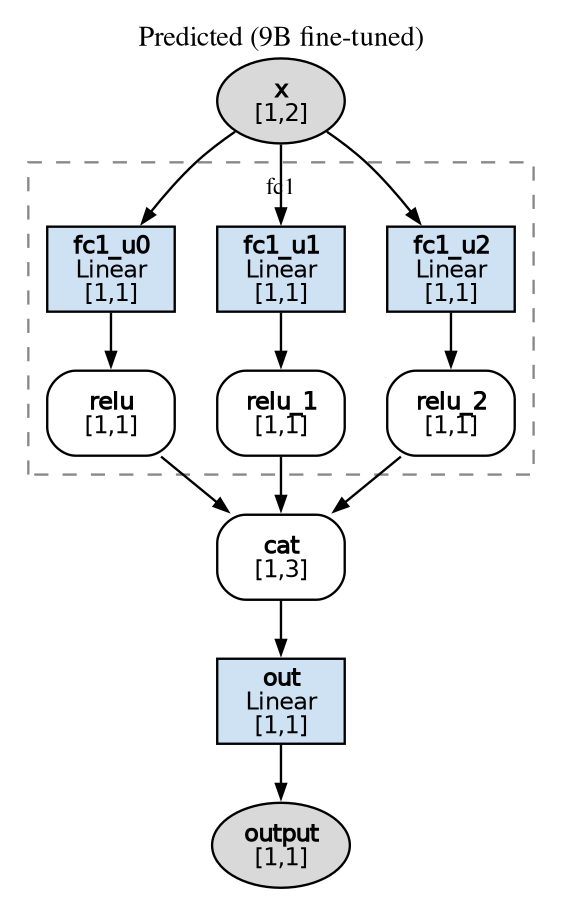
\includegraphics[width=\linewidth,height=0.40\textheight,keepaspectratio]{figs/ex01_ft9b_c_pred.png}\\\footnotesize 9B fine-tuned (exact)\end{minipage}\hfill
\caption{Example 1 (L0\_0803). Diff colours: black = matched, red dashed = missing (reference only), orange = hallucinated (prediction only), red text = wrong kind or shape.}
\end{figure}
\clearpage

\subsection{Example 2: A linear chain with dead code (tier L1)}\label{sec:ex02}
{\small set: official test \textbullet{} sample: \texttt{L1\_0886} \textbullet{} tier L1 \textbullet{} augmentation: \texttt{aug\_variant\_2} \textbullet{} topology seen in training \textbullet{} 6 nodes}

\lstinputlisting[style=py]{code/ex02.py}
\begin{center}\footnotesize\begin{tabular}{lcccccp{4.6cm}}\toprule
model & valid & edge F1 & exact & shape acc. & tokens & failure labels \\ \midrule
9B fine-tuned & yes & 1.00 & yes & 1.00 & 196 & \raggedright -- \tabularnewline
\bottomrule\end{tabular}\end{center}
\textbf{What to look at.} \texttt{self.unused\_op\_*} is declared and even \emph{called}, but its result never
reaches the \texttt{return}, so \texttt{torch.fx} (after dead-code elimination) does not contain it. The validator
checks exactly this (rule ``dead code included''). The fine-tuned model skips the dead call correctly. Over the whole test
set the base Coder-7B model included dead code in 34.6\% of the dead-code samples, the 9B 3-shot model in 0\%.

\begin{figure}[H]\centering
\begin{minipage}[b]{0.47\linewidth}\centering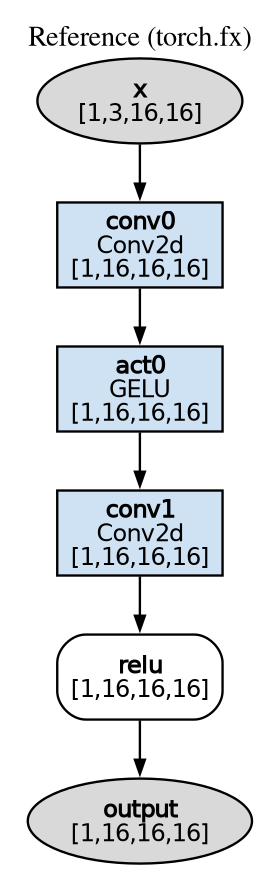
\includegraphics[width=\linewidth,height=0.40\textheight,keepaspectratio]{figs/ex02_ref.png}\\\footnotesize Reference (dead code removed)\end{minipage}\hfill
\begin{minipage}[b]{0.47\linewidth}\centering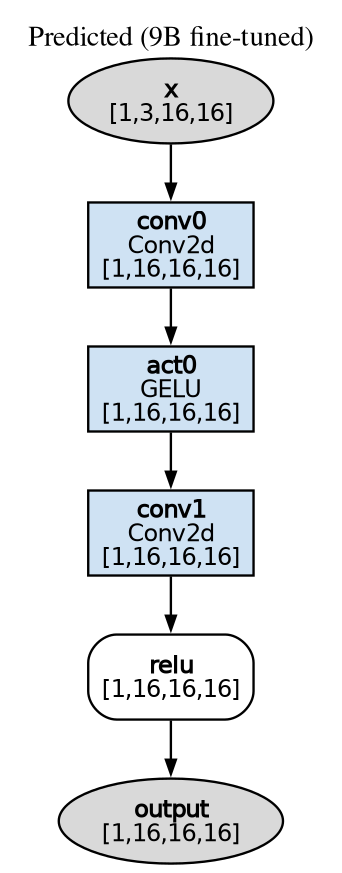
\includegraphics[width=\linewidth,height=0.40\textheight,keepaspectratio]{figs/ex02_ft9b_c_pred.png}\\\footnotesize 9B fine-tuned (exact)\end{minipage}\hfill
\caption{Example 2 (L1\_0886). Diff colours: black = matched, red dashed = missing (reference only), orange = hallucinated (prediction only), red text = wrong kind or shape.}
\end{figure}
\clearpage

\subsection{Example 3: A residual network (tier L2): the missing skip edge}\label{sec:ex03}
{\small set: official test \textbullet{} sample: \texttt{L2\_0804} \textbullet{} tier L2 \textbullet{} topology \textbf{held out} from training \textbullet{} 18 nodes}

\lstinputlisting[style=py]{code/ex03.py}
\begin{center}\footnotesize\begin{tabular}{lcccccp{4.6cm}}\toprule
model & valid & edge F1 & exact & shape acc. & tokens & failure labels \\ \midrule
9B 3-shot & no & 0.86 & no & 1.00 & 706 & \raggedright missing skip edge, missing edge, extra edge \tabularnewline
9B fine-tuned & yes & 1.00 & yes & 1.00 & 644 & \raggedright -- \tabularnewline
\bottomrule\end{tabular}\end{center}
\textbf{What to look at.} A residual network whose structure was \emph{held out} from fine-tuning. The 3-shot
base model gets every node right (node F1 1.0) but miswires the edges: the red dashed edges are reference edges it
missed (including the long \emph{skip connection} into an \texttt{add}), orange edges are ones it invented, and it emits
edges to node indices that do not exist (\texttt{edge [17, 18] points outside the 18 nodes}). Long-range skip edges
are the single most common failure of the prompted models (the \texttt{missing\_skip\_edge} label in Figure~\ref{fig:F7}).
The fine-tuned 9B gets this held-out topology exactly right.

\begin{figure}[H]\centering
\begin{minipage}[b]{0.47\linewidth}\centering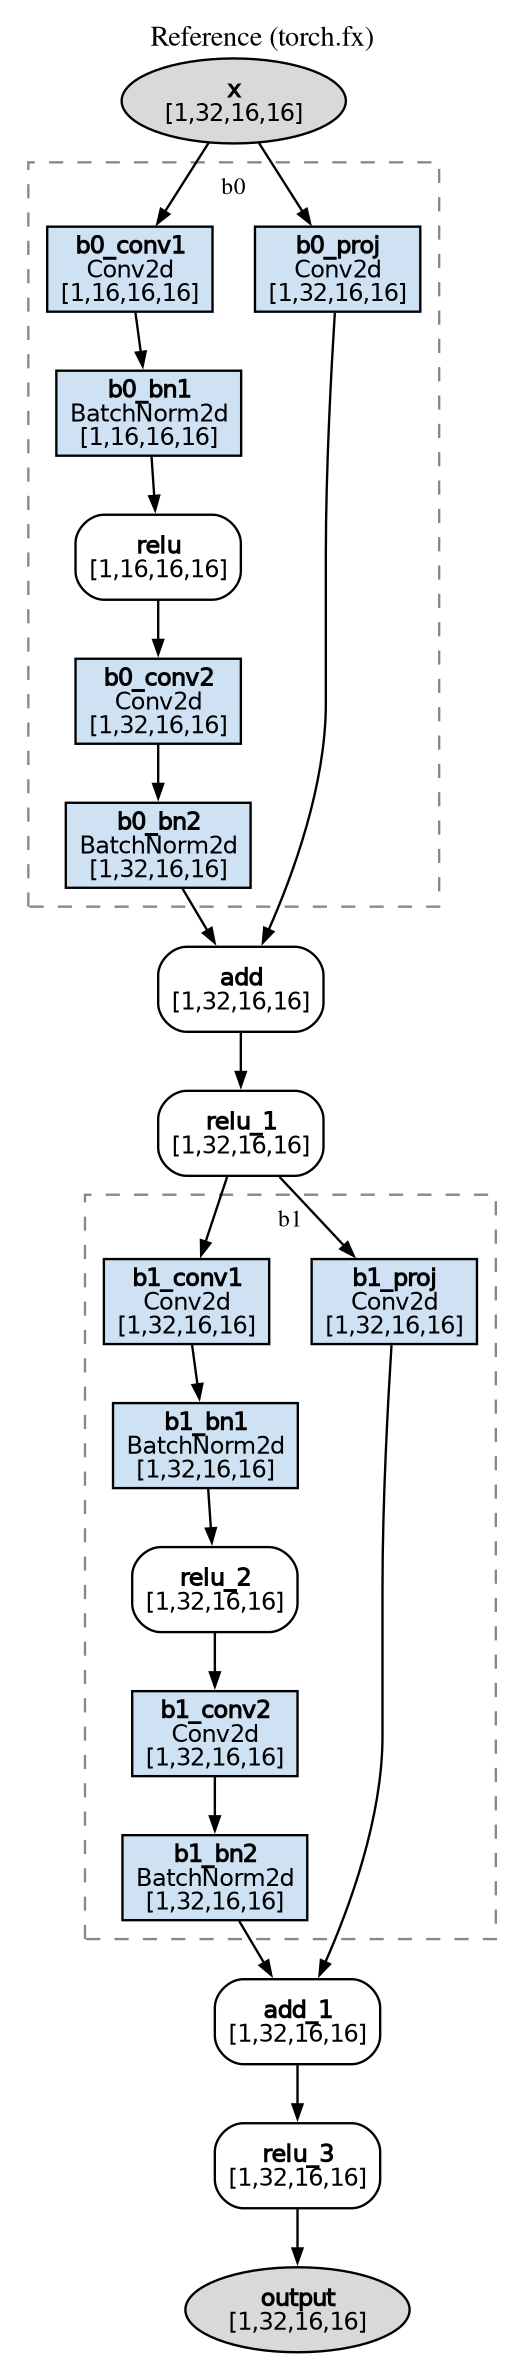
\includegraphics[width=\linewidth,height=0.40\textheight,keepaspectratio]{figs/ex03_ref.png}\\\footnotesize Reference\end{minipage}\hfill
\begin{minipage}[b]{0.47\linewidth}\centering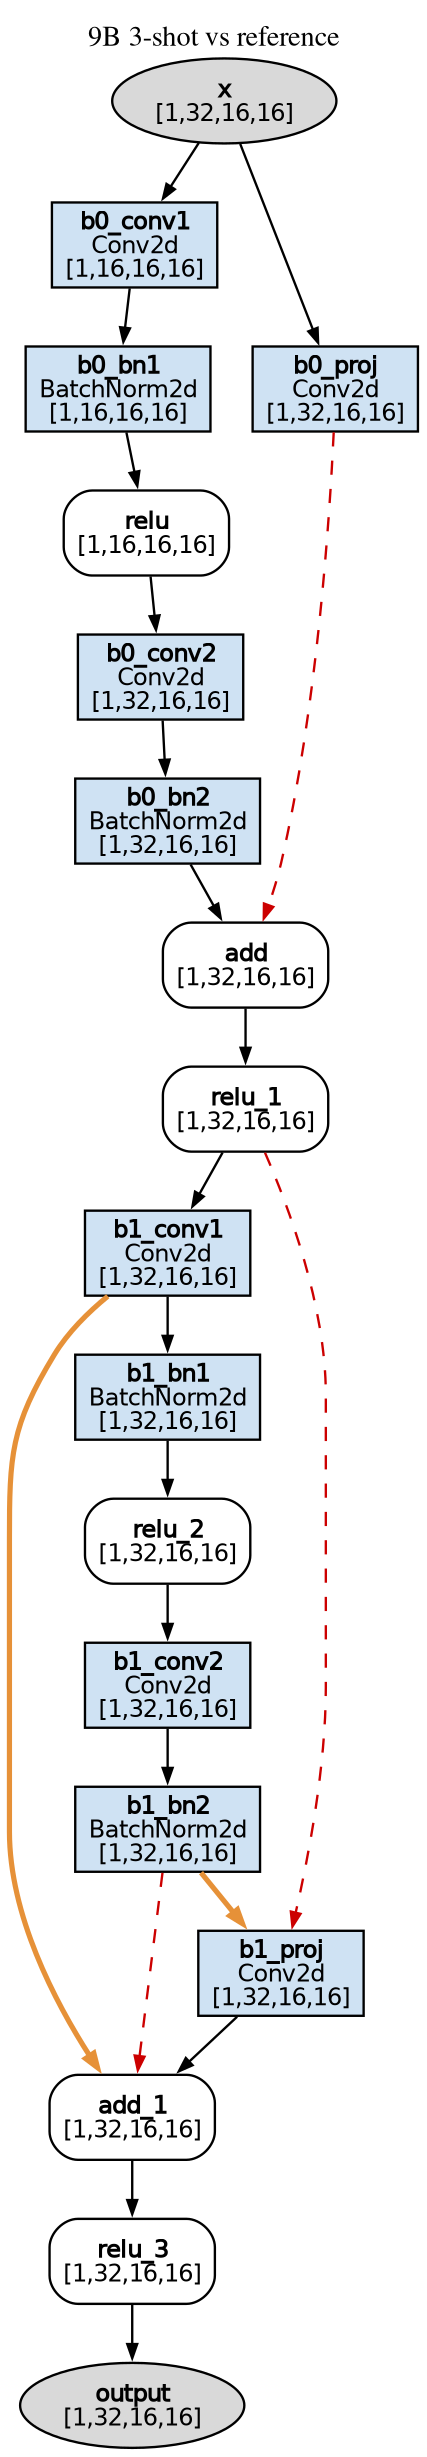
\includegraphics[width=\linewidth,height=0.40\textheight,keepaspectratio]{figs/ex03_base9b_fs_c_diff.png}\\\footnotesize 9B 3-shot vs reference\end{minipage}\hfill
\caption{Example 3 (L2\_0804). Diff colours: black = matched, red dashed = missing (reference only), orange = hallucinated (prediction only), red text = wrong kind or shape.}
\end{figure}
\clearpage

\subsection{Example 4: Parallel branches joined by concat (tier L3)}\label{sec:ex04}
{\small set: official test \textbullet{} sample: \texttt{L3\_0804} \textbullet{} tier L3 \textbullet{} topology seen in training \textbullet{} 12 nodes}

\lstinputlisting[style=py]{code/ex04.py}
\begin{center}\footnotesize\begin{tabular}{lcccccp{4.6cm}}\toprule
model & valid & edge F1 & exact & shape acc. & tokens & failure labels \\ \midrule
9B 3-shot & yes & 1.00 & yes & 1.00 & 405 & \raggedright -- \tabularnewline
\bottomrule\end{tabular}\end{center}
\textbf{What to look at.} Several parallel branches read the same tensor and are joined by
\texttt{torch.cat}. Branching and merging nodes are easy to spot in the drawing (out-degree $>1$, in-degree $>1$).
Here even the prompted 3-shot model is exactly right; tier L3 is the easiest multi-path tier for it (60.5\% exact).

\begin{figure}[H]\centering
\begin{minipage}[b]{0.47\linewidth}\centering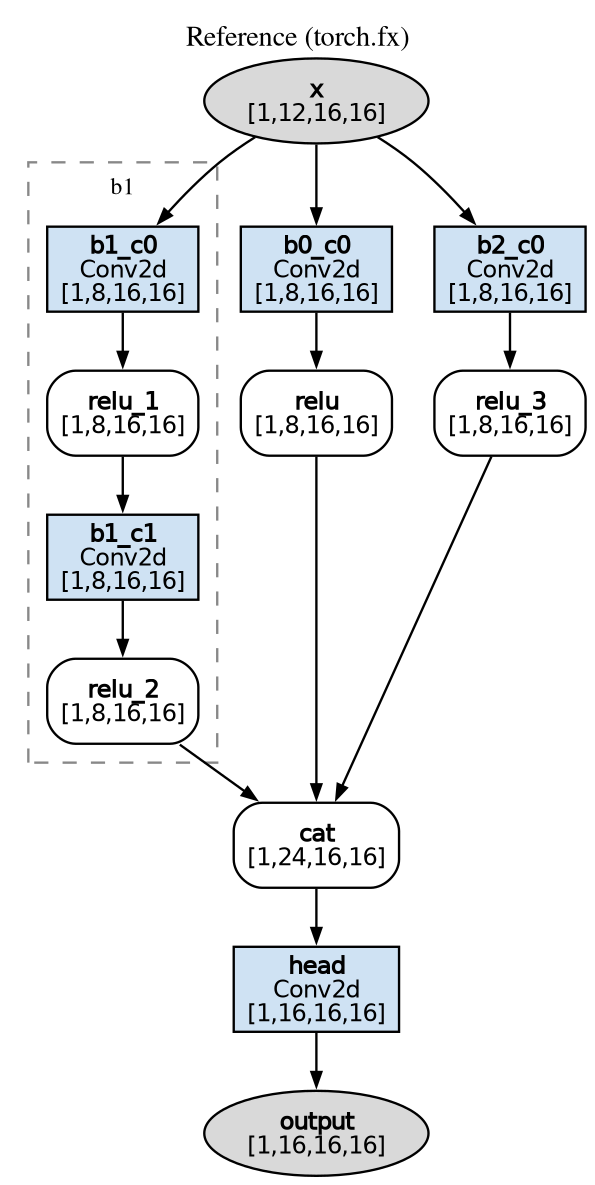
\includegraphics[width=\linewidth,height=0.40\textheight,keepaspectratio]{figs/ex04_ref.png}\\\footnotesize Reference\end{minipage}\hfill
\begin{minipage}[b]{0.47\linewidth}\centering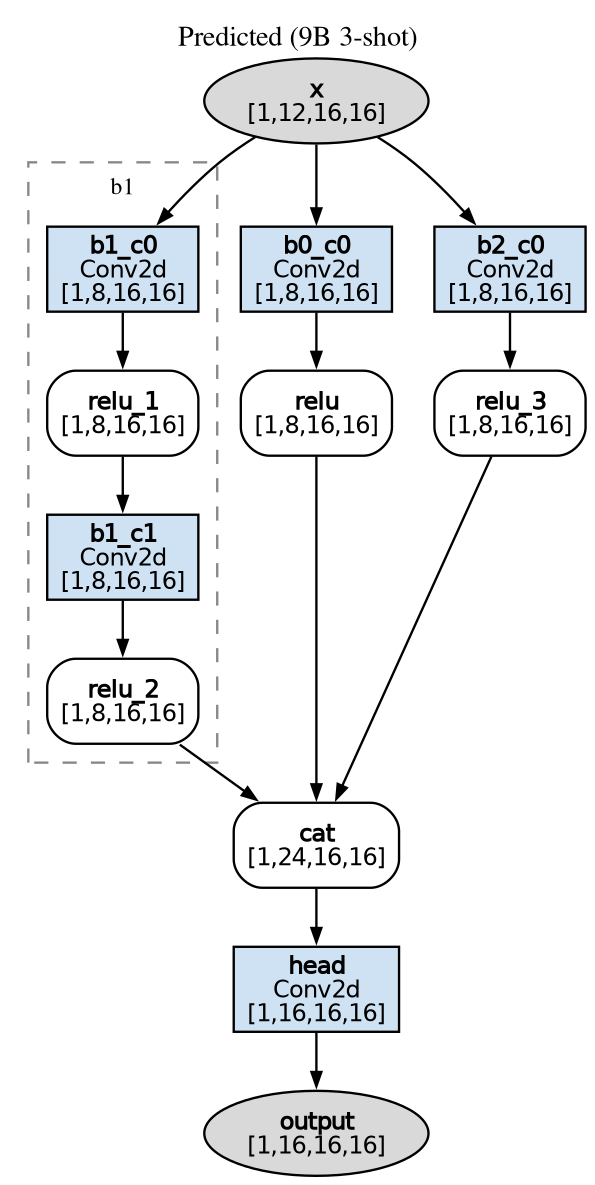
\includegraphics[width=\linewidth,height=0.40\textheight,keepaspectratio]{figs/ex04_base9b_fs_c_pred.png}\\\footnotesize 9B 3-shot (exact)\end{minipage}\hfill
\caption{Example 4 (L3\_0804). Diff colours: black = matched, red dashed = missing (reference only), orange = hallucinated (prediction only), red text = wrong kind or shape.}
\end{figure}
\clearpage

\subsection{Example 5: A held-out nested topology (tier L4): memorisation vs generalisation}\label{sec:ex05}
{\small set: official test \textbullet{} sample: \texttt{L4\_0800} \textbullet{} tier L4 \textbullet{} topology \textbf{held out} from training \textbullet{} 19 nodes}

\lstinputlisting[style=py]{code/ex05.py}
\begin{center}\footnotesize\begin{tabular}{lcccccp{4.6cm}}\toprule
model & valid & edge F1 & exact & shape acc. & tokens & failure labels \\ \midrule
2B fine-tuned & no & 0.92 & no & 1.00 & 638 & \raggedright missing skip edge, extra edge \tabularnewline
9B fine-tuned & yes & 1.00 & yes & 1.00 & 643 & \raggedright -- \tabularnewline
\bottomrule\end{tabular}\end{center}
\textbf{What to look at.} The nested L4 pattern (stem $\to$ two paths $\to$ concat $\to$ merge $\to$
residual add $\to$ head) with the one L4 structure that was held out of training. The fine-tuned \textbf{2B} writes
the nodes correctly but wires them like the L4 templates it saw in training: the validator reports
\texttt{'cat' has 1 input}, \texttt{'merge' has 2 inputs; a Conv2d takes exactly 1} and \texttt{'add' has 1 input
(missing skip edge?)}. All 52 held-out L4 test samples fail this way for the 2B (0\%), while the fine-tuned
\textbf{9B} gets 100\% of them. This is the clearest memorisation-vs-generalisation contrast in the project.

\begin{figure}[H]\centering
\begin{minipage}[b]{0.47\linewidth}\centering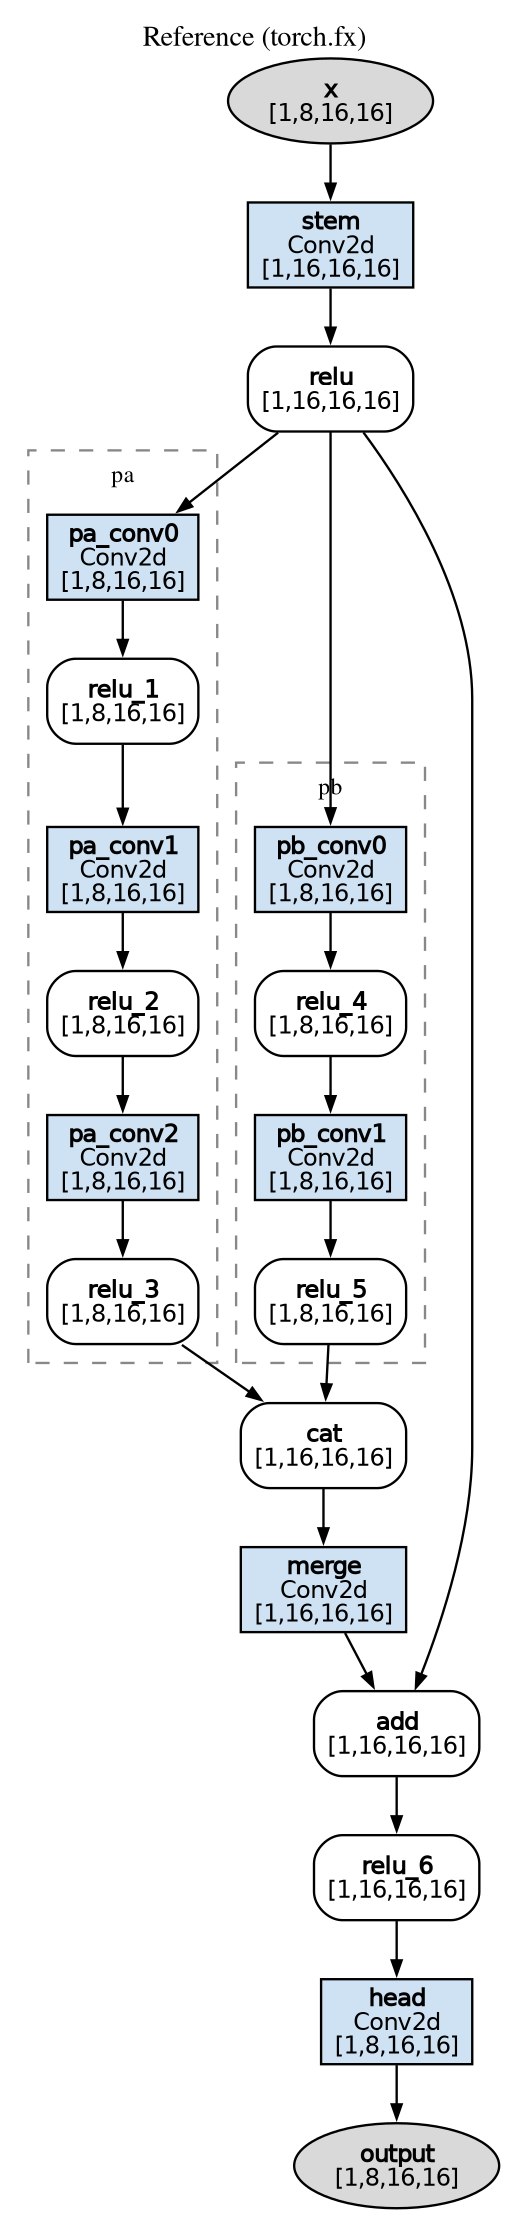
\includegraphics[width=\linewidth,height=0.40\textheight,keepaspectratio]{figs/ex05_ref.png}\\\footnotesize Reference\end{minipage}\hfill
\begin{minipage}[b]{0.47\linewidth}\centering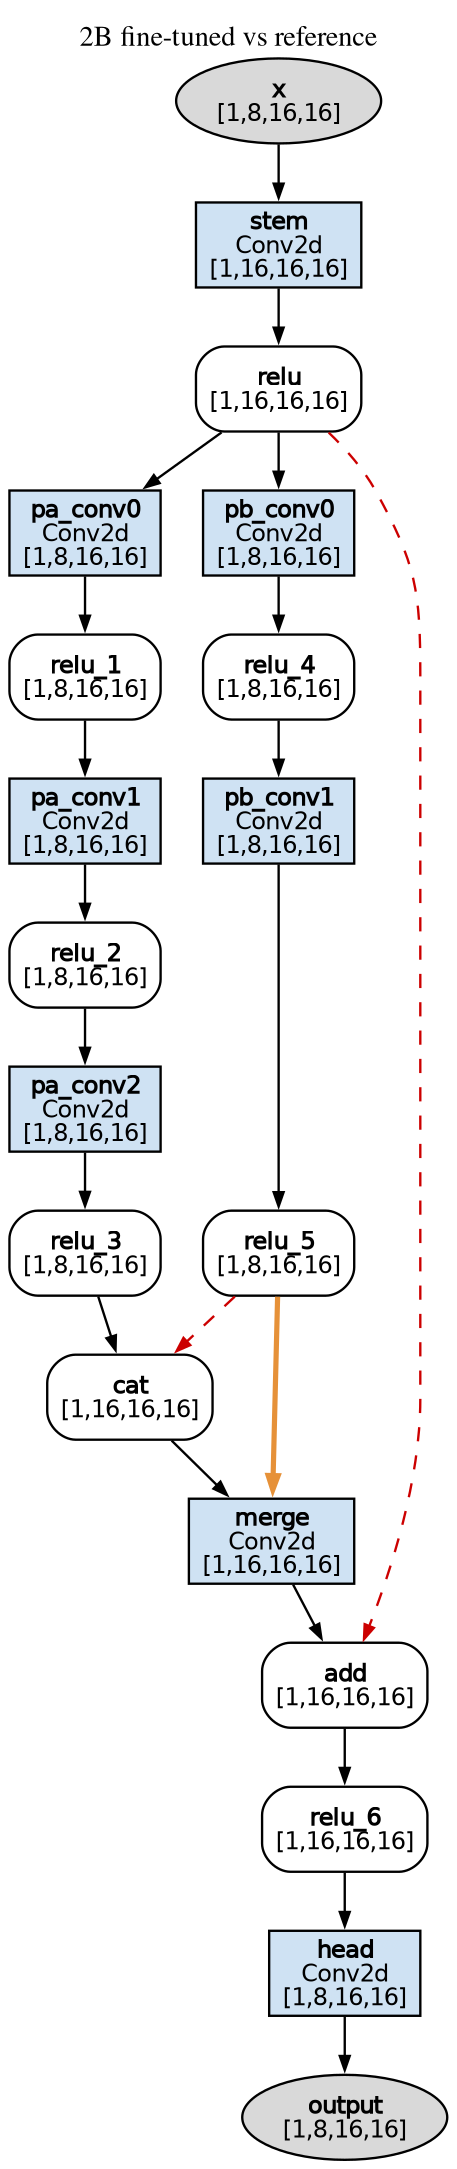
\includegraphics[width=\linewidth,height=0.40\textheight,keepaspectratio]{figs/ex05_ft2b_c_diff.png}\\\footnotesize 2B fine-tuned vs reference\end{minipage}\hfill
\caption{Example 5 (L4\_0800). Diff colours: black = matched, red dashed = missing (reference only), orange = hallucinated (prediction only), red text = wrong kind or shape.}
\end{figure}
\clearpage

\subsection{Example 6: The zero-shot runaway loop}\label{sec:ex06}
{\small set: official test \textbullet{} sample: \texttt{L0\_0857} \textbullet{} tier L0 \textbullet{} augmentation: \texttt{aug\_variant\_1} \textbullet{} topology seen in training \textbullet{} 14 nodes}

\lstinputlisting[style=py]{code/ex06.py}
\begin{center}\footnotesize\begin{tabular}{lcccccp{4.6cm}}\toprule
model & valid & edge F1 & exact & shape acc. & tokens & failure labels \\ \midrule
9B zero-shot & no & 0.00 & no & 0.00 & 3072 & \raggedright parse fail \tabularnewline
\bottomrule\end{tabular}\end{center}
\textbf{What to look at.} Nothing is wrong with the code; the failure is in decoding. The zero-shot 9B starts
a plausible answer, then falls into a loop in the edge list (\texttt{[n,n+1]} with ever larger \texttt{n}) until the
3{,}072-token limit stops it. The output is not a usable graph (parse/schema failure). 22\% of zero-shot test answers
ended like this (mostly on the larger L2/L4 graphs); fine-tuned models never did (Section~\ref{sec:journey}).

\begin{figure}[H]\centering
\begin{minipage}[b]{0.55\linewidth}\centering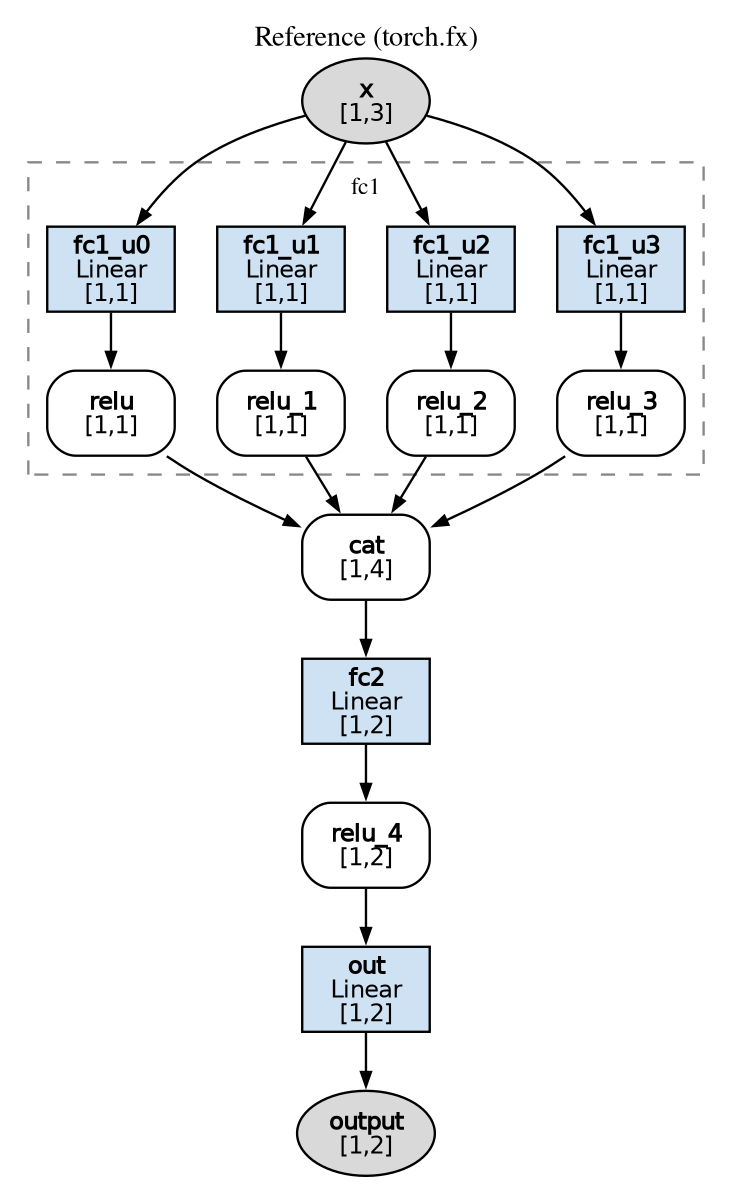
\includegraphics[width=\linewidth,height=0.36\textheight,keepaspectratio]{figs/ex06_ref.png}\\\footnotesize Reference\end{minipage}\hfill
\caption{Example 6 (L0\_0857). Diff colours: black = matched, red dashed = missing (reference only), orange = hallucinated (prediction only), red text = wrong kind or shape.}
\end{figure}
\noindent\textit{End of the zero-shot answer (cut off at 3{,}072 tokens):}
\begin{lstlisting}[style=plain]
..., 354], [354, 355], [355, 356], [356, 357], [357, 358], [358, 359], [359, 360], [360, 361], [361, 362], [362, 363], [363, 364], [364, 365], [365, 366], [366, 367], [367, 368], [368, 369], [369, 370], [370, 371], [371, 372], [372, 
\end{lstlisting}
\clearpage

\subsection{Example 7: OOD: nested submodules (dotted scopes)}\label{sec:ex07}
{\small set: OOD-1 \textbullet{} sample: \texttt{OOD\_resnet\_nested\_2} \textbullet{} category: \texttt{nested\_basicblock} \textbullet{} 13 nodes}

\lstinputlisting[style=py]{code/ex07.py}
\begin{center}\footnotesize\begin{tabular}{lcccccp{4.6cm}}\toprule
model & valid & edge F1 & exact & shape acc. & tokens & failure labels \\ \midrule
9B fine-tuned & no & 0.27 & no & 1.00 & 256 & \raggedright missing skip edge, missing edge, extra edge, missing node \tabularnewline
9B FT + synthetic & yes & 1.00 & yes & 1.00 & 435 & \raggedright -- \tabularnewline
\bottomrule\end{tabular}\end{center}
\textbf{What to look at.} An out-of-distribution module: a \emph{submodule class} \texttt{ResUnit} used twice.
\texttt{torch.fx} inlines nested modules and names their layers with the full path (\texttt{unit\_a\_conv\_a},
scope \texttt{unit\_a.conv\_a}). The dataset only has flat models, so the fine-tuned 9B writes \texttt{conv\_a} (a
name that is not declared at the top level: the validator flags it as possibly hallucinated) and collapses the two
units into one (the whole second unit is red dashed = missing). After adding synthetic training modules that contain
nested classes, the model gets it exactly right.

\begin{figure}[H]\centering
\begin{minipage}[b]{0.32\linewidth}\centering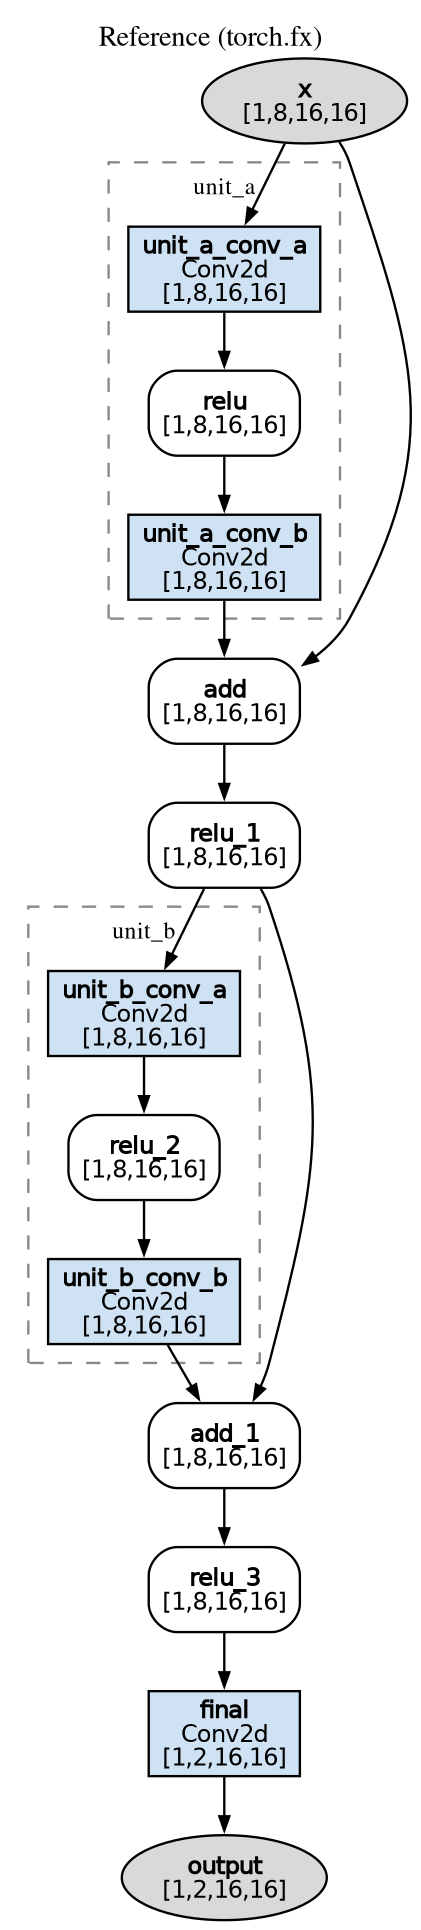
\includegraphics[width=\linewidth,height=0.40\textheight,keepaspectratio]{figs/ex07_ref.png}\\\footnotesize Reference\end{minipage}\hfill
\begin{minipage}[b]{0.32\linewidth}\centering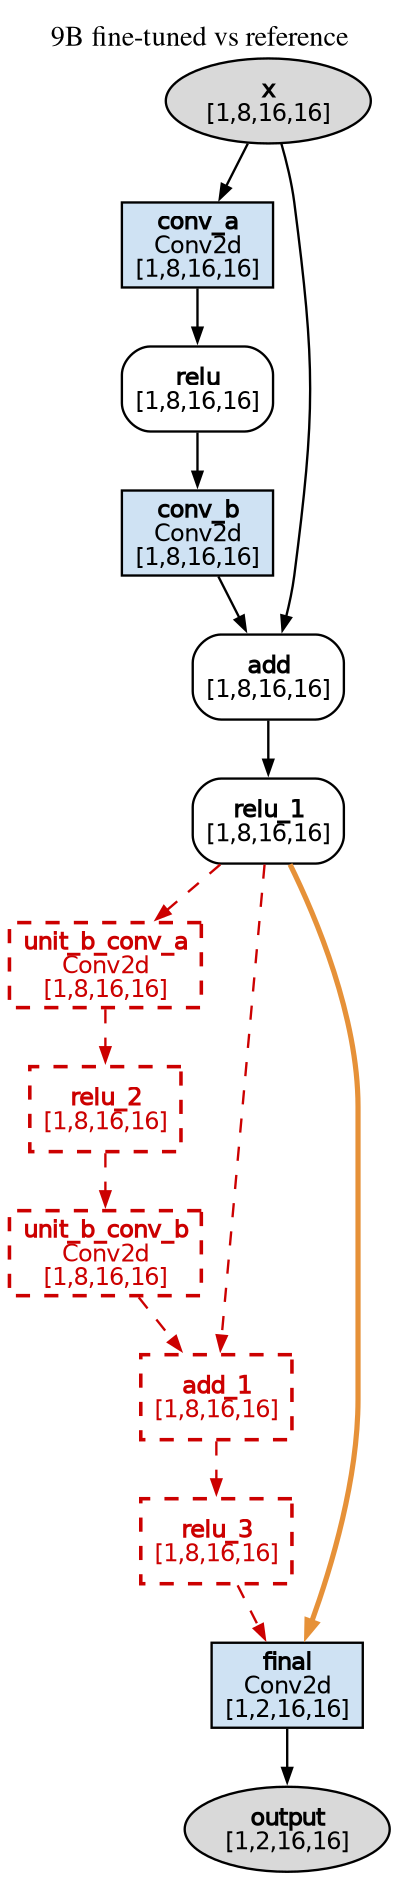
\includegraphics[width=\linewidth,height=0.40\textheight,keepaspectratio]{figs/ex07_ft9b_c_diff.png}\\\footnotesize 9B fine-tuned vs reference\end{minipage}\hfill
\begin{minipage}[b]{0.32\linewidth}\centering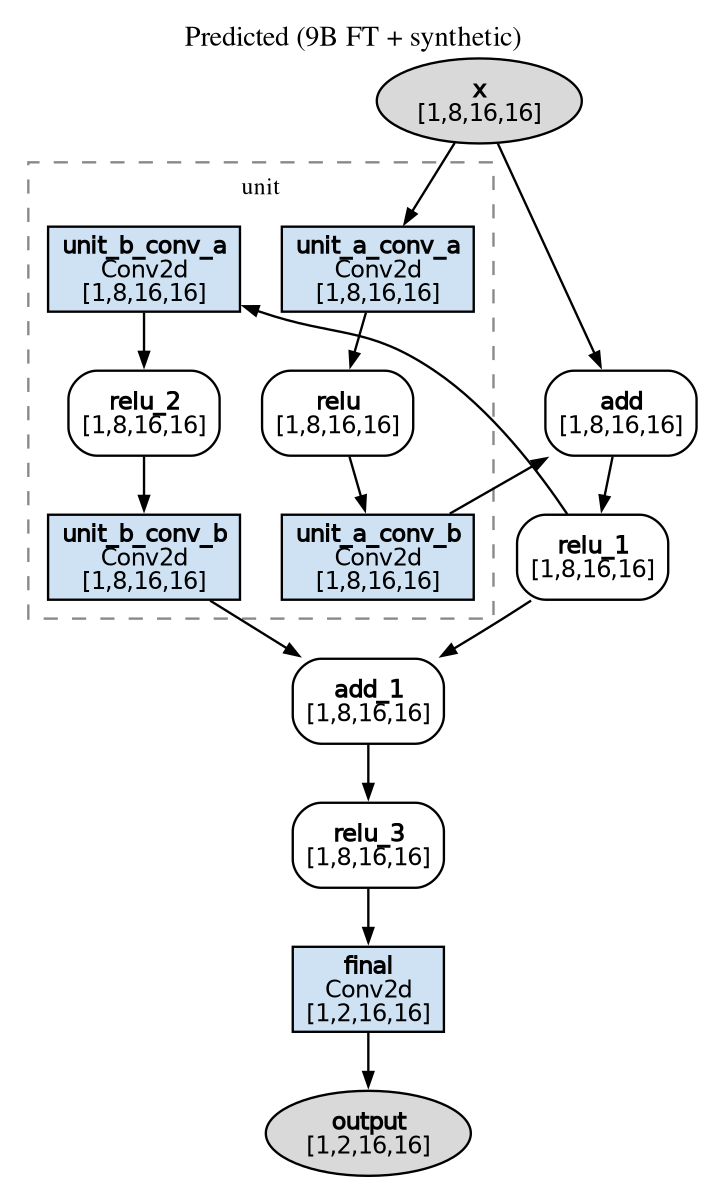
\includegraphics[width=\linewidth,height=0.40\textheight,keepaspectratio]{figs/ex07_ft9b_aug_c_pred.png}\\\footnotesize 9B FT + synthetic (exact)\end{minipage}\hfill
\caption{Example 7 (OOD\_resnet\_nested\_2). Diff colours: black = matched, red dashed = missing (reference only), orange = hallucinated (prediction only), red text = wrong kind or shape.}
\end{figure}
\clearpage

\subsection{Example 8: OOD: an nn.ModuleList loop}\label{sec:ex08}
{\small set: OOD-1 \textbullet{} sample: \texttt{OOD\_modulelist\_1} \textbullet{} category: \texttt{modulelist} \textbullet{} 9 nodes}

\lstinputlisting[style=py]{code/ex08.py}
\begin{center}\footnotesize\begin{tabular}{lcccccp{4.6cm}}\toprule
model & valid & edge F1 & exact & shape acc. & tokens & failure labels \\ \midrule
9B fine-tuned & no & 0.75 & no & 1.00 & 226 & \raggedright naming only \tabularnewline
9B FT + synthetic & yes & 1.00 & yes & 1.00 & 228 & \raggedright -- \tabularnewline
\bottomrule\end{tabular}\end{center}
\textbf{What to look at.} \texttt{nn.ModuleList} plus a Python \texttt{for} loop: \texttt{torch.fx}
unrolls the loop and names the layers \texttt{layers\_0}, \texttt{layers\_1}, \texttt{layers\_2}. The fine-tuned 9B
draws the right structure (isomorphic) but names the nodes \texttt{layers}, \texttt{layers\_1}, \dots, so strict
metrics and the code-consistency check fail (``naming only'' failure). The synthetic-data model names them correctly.

\begin{figure}[H]\centering
\begin{minipage}[b]{0.32\linewidth}\centering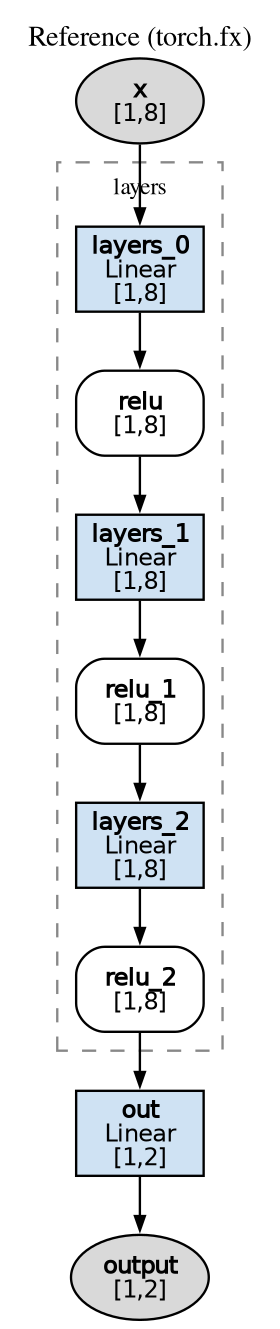
\includegraphics[width=\linewidth,height=0.40\textheight,keepaspectratio]{figs/ex08_ref.png}\\\footnotesize Reference\end{minipage}\hfill
\begin{minipage}[b]{0.32\linewidth}\centering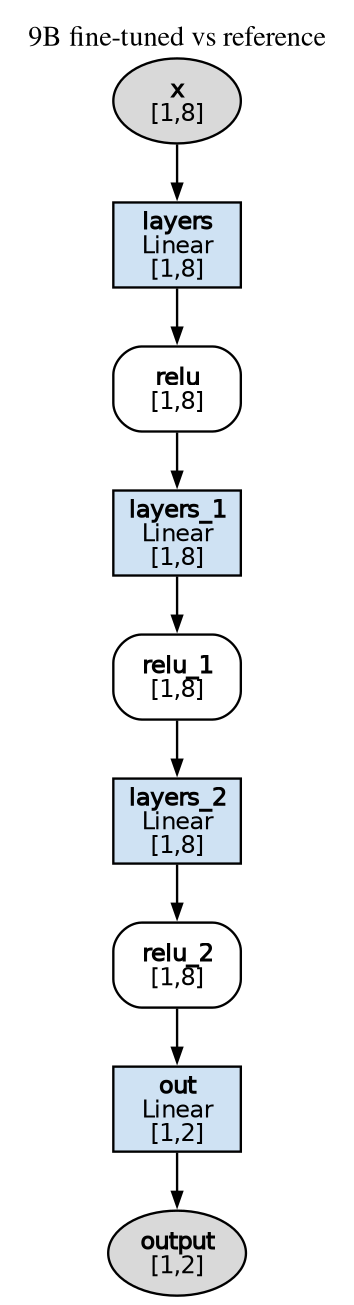
\includegraphics[width=\linewidth,height=0.40\textheight,keepaspectratio]{figs/ex08_ft9b_c_diff.png}\\\footnotesize 9B fine-tuned vs reference\end{minipage}\hfill
\begin{minipage}[b]{0.32\linewidth}\centering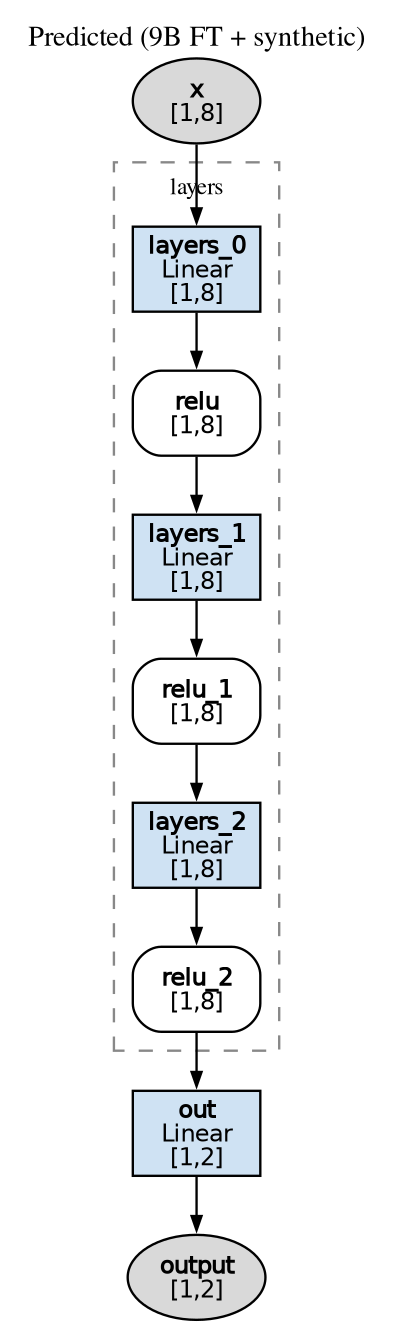
\includegraphics[width=\linewidth,height=0.40\textheight,keepaspectratio]{figs/ex08_ft9b_aug_c_pred.png}\\\footnotesize 9B FT + synthetic (exact)\end{minipage}\hfill
\caption{Example 8 (OOD\_modulelist\_1). Diff colours: black = matched, red dashed = missing (reference only), orange = hallucinated (prediction only), red text = wrong kind or shape.}
\end{figure}
\clearpage

\subsection{Example 9: OOD: Squeeze-and-Excitation, fixed by verify-and-retry}\label{sec:ex09}
{\small set: OOD-1 \textbullet{} sample: \texttt{OOD\_se\_1} \textbullet{} category: \texttt{squeeze\_excite} \textbullet{} 12 nodes}

\lstinputlisting[style=py]{code/ex09.py}
\begin{center}\footnotesize\begin{tabular}{lcccccp{4.6cm}}\toprule
model & valid & edge F1 & exact & shape acc. & tokens & failure labels \\ \midrule
9B FT, before/after retry & yes & 0.87 & no & 0.91 & 635 & \raggedright missing edge, extra edge, missing node \tabularnewline
\bottomrule\end{tabular}\end{center}
\textbf{What to look at.} \emph{Verify-and-retry}: the validator's messages (which never use the reference)
are sent back to the model as a new chat turn. The first attempt left the output node disconnected
(\texttt{output node needs >=1 input}, \texttt{node 0 'x' does not lead to the output}). After one retry round the graph
passes every validity check, but it is \emph{still not exactly right} (edge F1 0.87, one node missing): a valid graph
is not necessarily a correct graph. Over OOD-1, retry raised the fine-tuned 9B from 47.5\% to 67.5\% valid and from
30\% to 45\% exact.

\begin{figure}[H]\centering
\begin{minipage}[b]{0.32\linewidth}\centering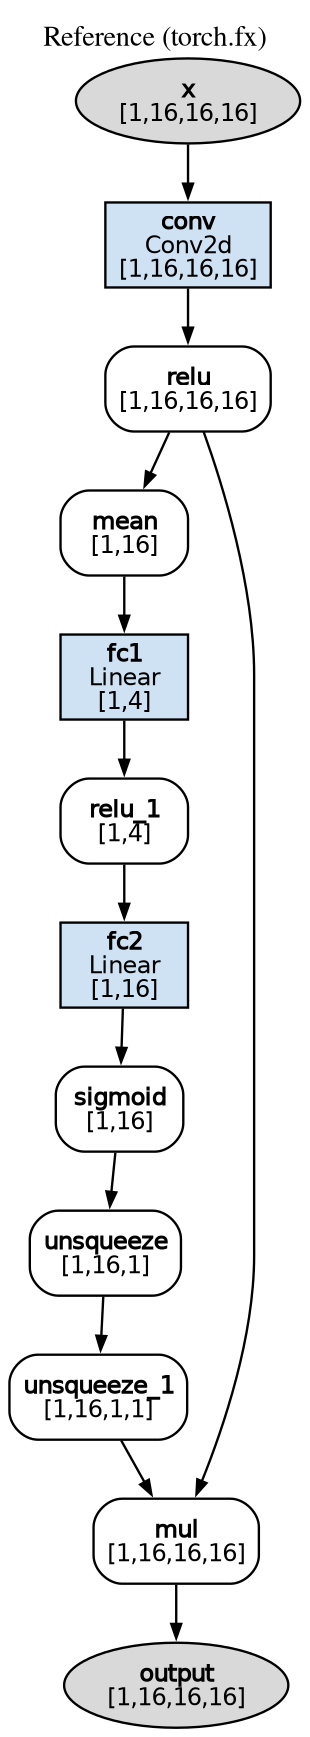
\includegraphics[width=\linewidth,height=0.40\textheight,keepaspectratio]{figs/ex09_ref.png}\\\footnotesize Reference\end{minipage}\hfill
\begin{minipage}[b]{0.32\linewidth}\centering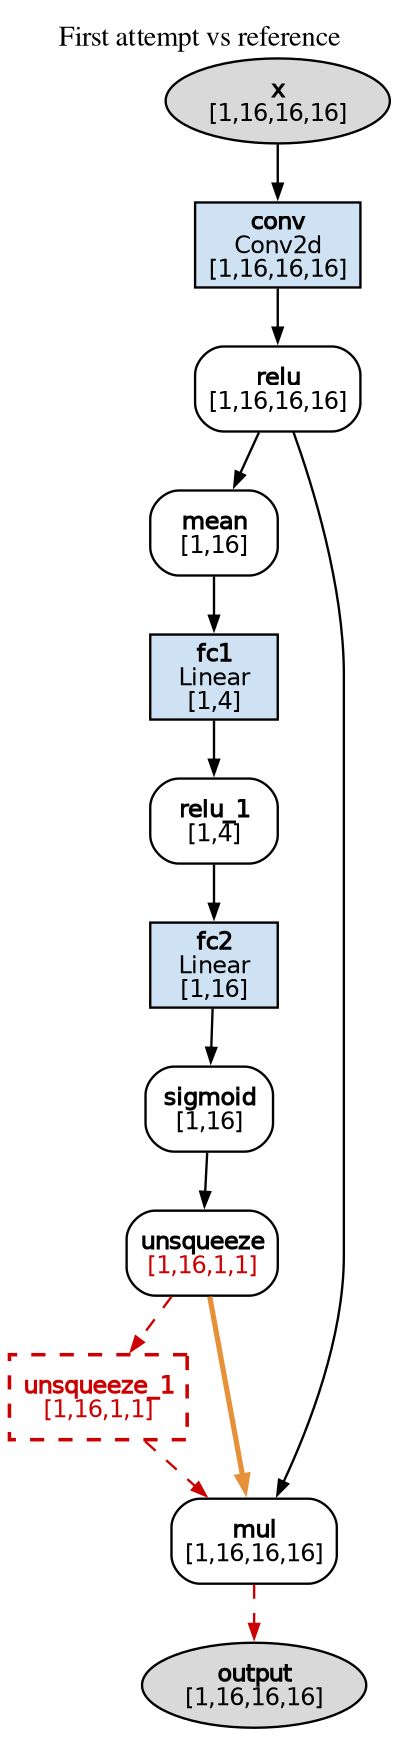
\includegraphics[width=\linewidth,height=0.40\textheight,keepaspectratio]{figs/ex09_ft9b_c_retry_initial_diff.png}\\\footnotesize first attempt vs reference\end{minipage}\hfill
\begin{minipage}[b]{0.32\linewidth}\centering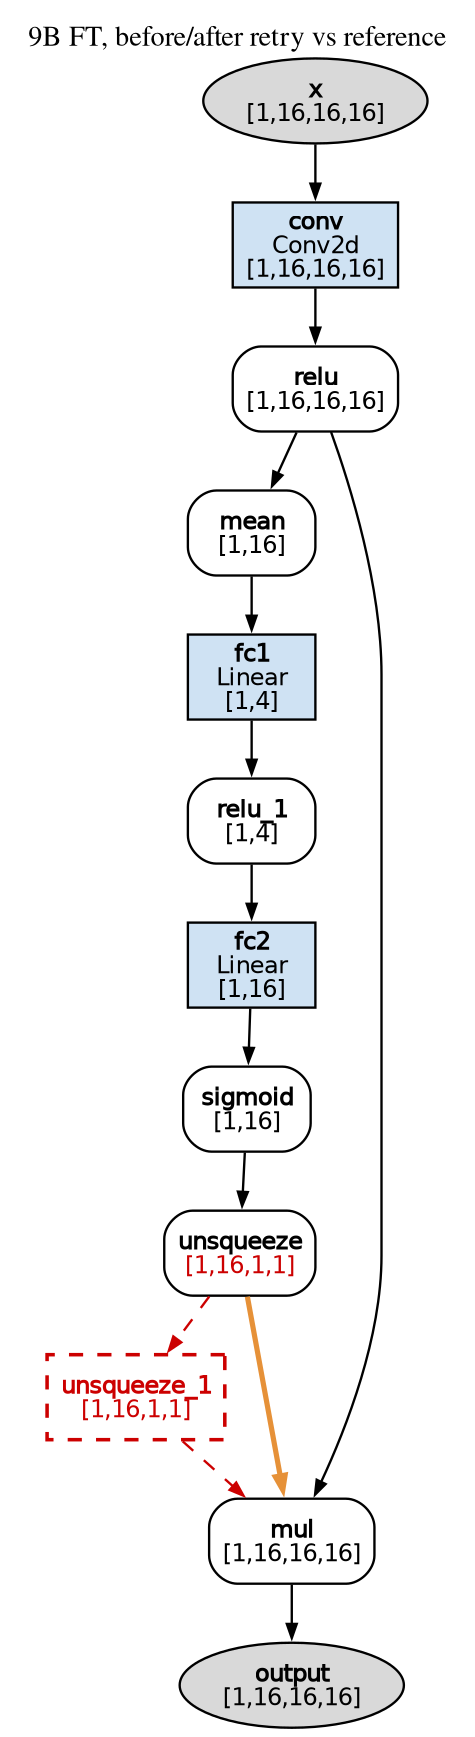
\includegraphics[width=\linewidth,height=0.40\textheight,keepaspectratio]{figs/ex09_ft9b_c_retry_diff.png}\\\footnotesize after 1 retry round\end{minipage}\hfill
\caption{Example 9 (OOD\_se\_1). Diff colours: black = matched, red dashed = missing (reference only), orange = hallucinated (prediction only), red text = wrong kind or shape.}
\end{figure}
\clearpage

\subsection{Example 10: OOD-2: a transposed-convolution decoder (shape failure)}\label{sec:ex10}
{\small set: OOD-2 \textbullet{} sample: \texttt{OOD2\_deconv\_2} \textbullet{} category: \texttt{transposed\_conv} \textbullet{} 9 nodes}

\lstinputlisting[style=py]{code/ex10.py}
\begin{center}\footnotesize\begin{tabular}{lcccccp{4.6cm}}\toprule
model & valid & edge F1 & exact & shape acc. & tokens & failure labels \\ \midrule
9B FT + synthetic & no & 1.00 & yes & 0.11 & 291 & \raggedright shape only \tabularnewline
27B 3-shot & yes & 1.00 & yes & 1.00 & 281 & \raggedright -- \tabularnewline
\bottomrule\end{tabular}\end{center}
\textbf{What to look at.} OOD-2 deliberately uses operators that appear in neither the dataset nor the
synthetic generator, here \texttt{nn.ConvTranspose2d} (an up-sampling convolution). The synthetic-data 9B gets the
\emph{topology} exactly right (all edges black) but almost all \emph{shapes} wrong (red shape text, shape accuracy
11\%). The mistake starts at the very first layer: the model ignores the \texttt{stride=2} of the ordinary
convolution \texttt{down} and predicts \texttt{[1,8,16,16]} instead of \texttt{[1,8,8,8]}. Every later shape inherits
the error, so the transposed convolution then ``doubles'' 16 to 32 instead of 8 to 16. The shape check catches the
inconsistency at the final skip addition (\texttt{add\_1 inputs [1,4,16,16] and [1,4,32,32] are not
broadcast-compatible}). The 27B model gets
this one fully right. Shape propagation through unseen operators is the main remaining weakness of all fine-tuned
models.

\begin{figure}[H]\centering
\begin{minipage}[b]{0.47\linewidth}\centering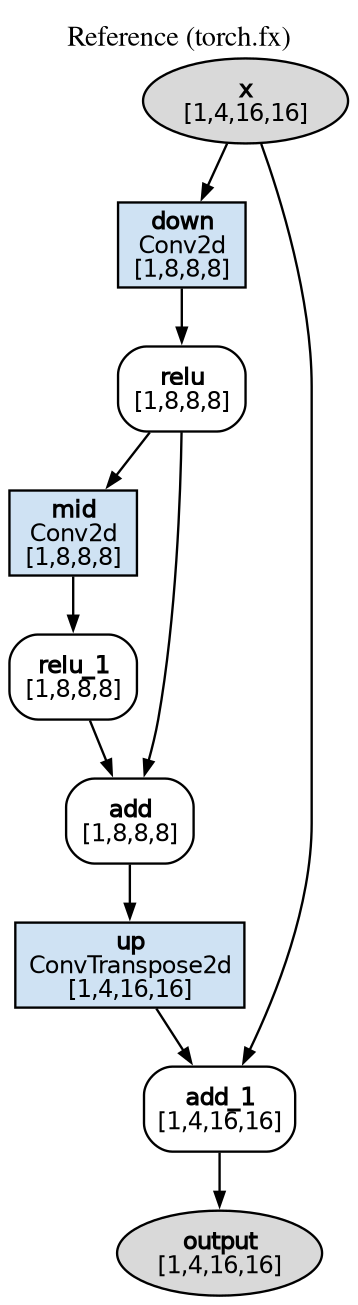
\includegraphics[width=\linewidth,height=0.40\textheight,keepaspectratio]{figs/ex10_ref.png}\\\footnotesize Reference\end{minipage}\hfill
\begin{minipage}[b]{0.47\linewidth}\centering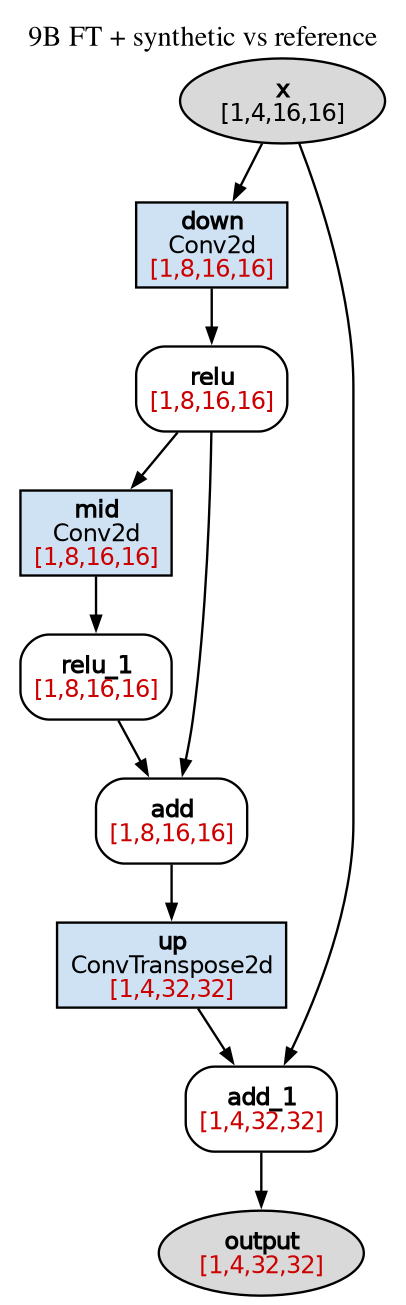
\includegraphics[width=\linewidth,height=0.40\textheight,keepaspectratio]{figs/ex10_ft9b_aug_c_diff.png}\\\footnotesize 9B FT + synthetic vs reference\end{minipage}\hfill
\caption{Example 10 (OOD2\_deconv\_2). Diff colours: black = matched, red dashed = missing (reference only), orange = hallucinated (prediction only), red text = wrong kind or shape.}
\end{figure}
\clearpage

\subsection{Example 11: OOD-2: attention with matmul and softmax}\label{sec:ex11}
{\small set: OOD-2 \textbullet{} sample: \texttt{OOD2\_attn\_1} \textbullet{} category: \texttt{matmul\_attention} \textbullet{} 13 nodes}

\lstinputlisting[style=py]{code/ex11.py}
\begin{center}\footnotesize\begin{tabular}{lcccccp{4.6cm}}\toprule
model & valid & edge F1 & exact & shape acc. & tokens & failure labels \\ \midrule
9B FT + synthetic & yes & 1.00 & yes & 1.00 & 349 & \raggedright -- \tabularnewline
27B 3-shot & no & 1.00 & yes & 0.69 & 355 & \raggedright shape only \tabularnewline
\bottomrule\end{tabular}\end{center}
\textbf{What to look at.} A tiny attention block (\texttt{unsqueeze}, \texttt{matmul}, \texttt{softmax},
\texttt{squeeze}; method calls become \texttt{call\_method} nodes). Here the roles flip: the synthetic-data 9B is
exactly right, while the 27B gets the topology right but adds an edge to a node index that does not exist and gets 31\%
of the shapes wrong, so the validator rejects it. Bigger is better on average, not on every example.

\begin{figure}[H]\centering
\begin{minipage}[b]{0.32\linewidth}\centering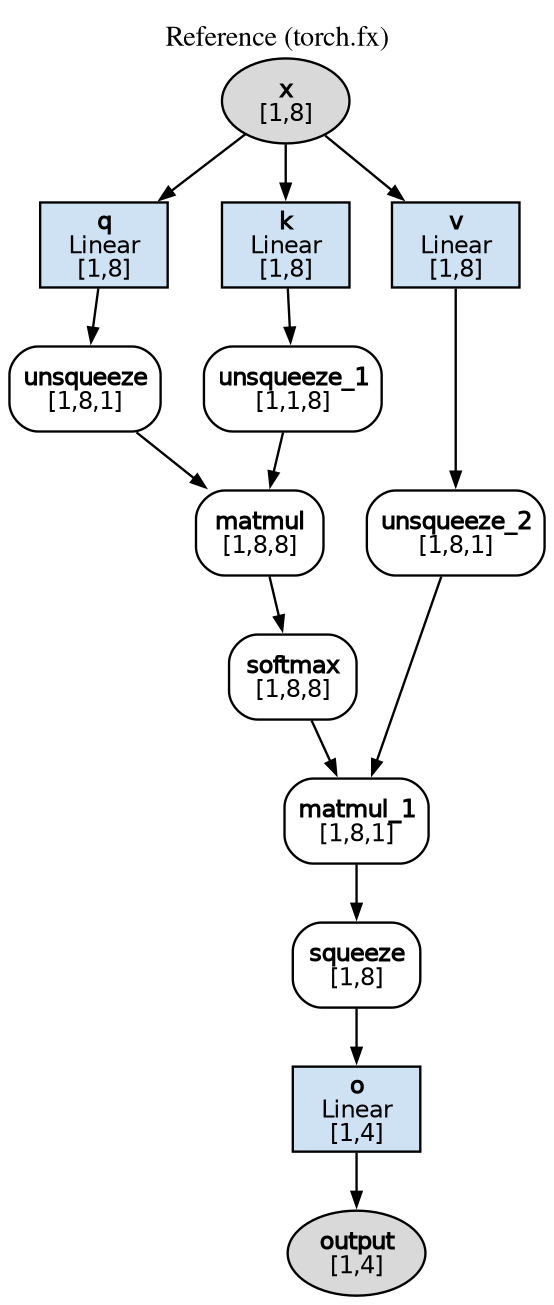
\includegraphics[width=\linewidth,height=0.40\textheight,keepaspectratio]{figs/ex11_ref.png}\\\footnotesize Reference\end{minipage}\hfill
\begin{minipage}[b]{0.32\linewidth}\centering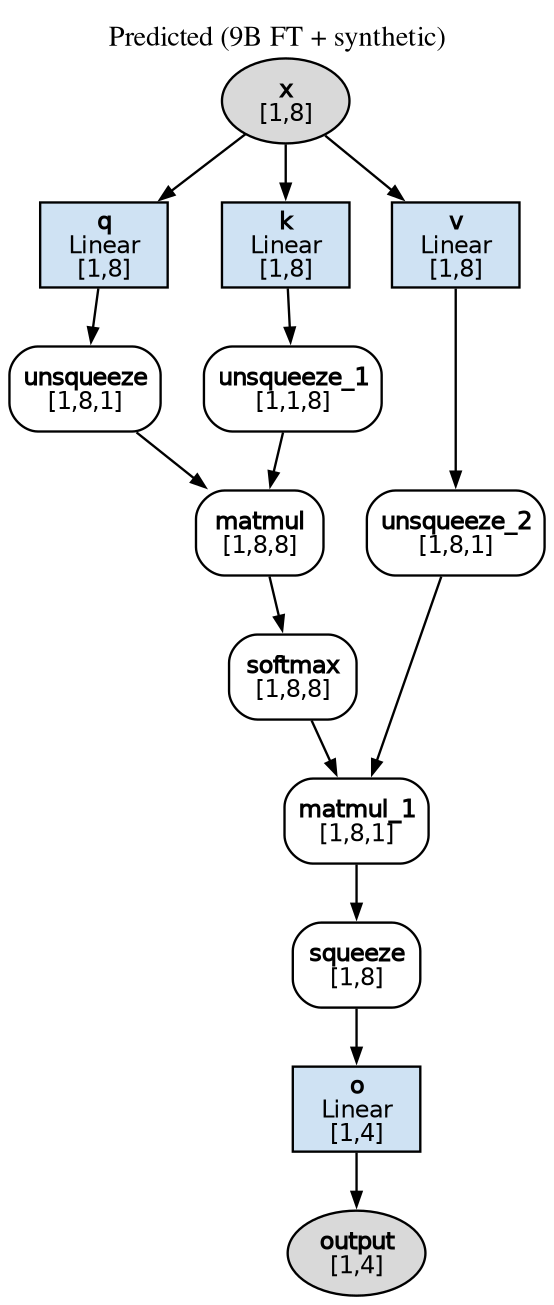
\includegraphics[width=\linewidth,height=0.40\textheight,keepaspectratio]{figs/ex11_ft9b_aug_c_pred.png}\\\footnotesize 9B FT + synthetic (exact)\end{minipage}\hfill
\begin{minipage}[b]{0.32\linewidth}\centering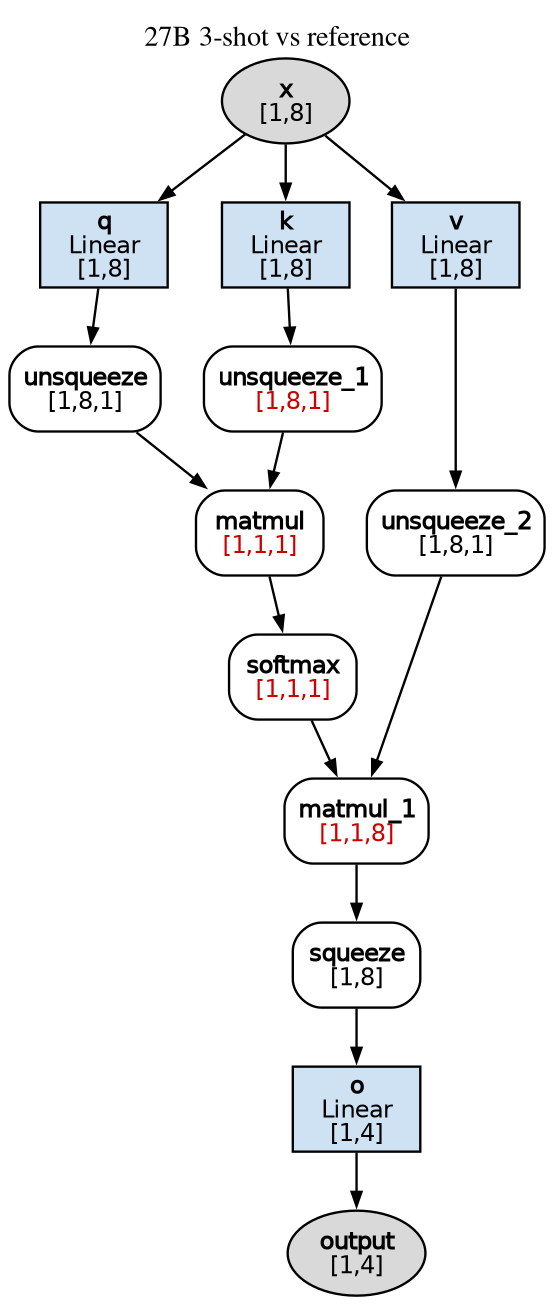
\includegraphics[width=\linewidth,height=0.40\textheight,keepaspectratio]{figs/ex11_ceil_fs_c_diff.png}\\\footnotesize 27B 3-shot vs reference\end{minipage}\hfill
\caption{Example 11 (OOD2\_attn\_1). Diff colours: black = matched, red dashed = missing (reference only), orange = hallucinated (prediction only), red text = wrong kind or shape.}
\end{figure}
\clearpage

\subsection{Example 12: Untraceable code: no torch.fx reference exists}\label{sec:ex12}
{\small set: untraceable set \textbullet{} sample: \texttt{UNT\_data\_dependent\_if} \textbullet{} category: \texttt{untraceable}}

\lstinputlisting[style=py]{code/ex12.py}
\begin{center}\footnotesize\begin{tabular}{lcccccp{4.6cm}}\toprule
model & valid & edge F1 & exact & shape acc. & tokens & failure labels \\ \midrule
9B fine-tuned & no & -- & n/a & -- & 160 & \raggedright n/a \tabularnewline
\bottomrule\end{tabular}\end{center}
\textbf{What to look at.} The \texttt{if} depends on the \emph{value} of the input, so
\texttt{torch.fx.symbolic\_trace} raises \texttt{TraceError}: there is no reference graph, and this is exactly where an
LLM can still be useful. The fine-tuned 9B draws both branches feeding the output (it cannot know which branch runs),
which the validator reports as \texttt{output node has 2 inputs}. The validator also wrongly reports \texttt{conv} as
dead code: its code analysis only follows straight-line code and does not look inside \texttt{if} bodies (a known
limitation, Section~\ref{sec:caveats}). These examples are qualitative only.

\begin{figure}[H]\centering
\begin{minipage}[b]{0.55\linewidth}\centering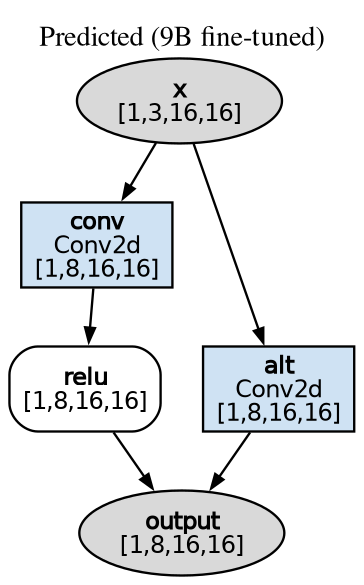
\includegraphics[width=\linewidth,height=0.36\textheight,keepaspectratio]{figs/ex12_ft9b_c_pred.png}\\\footnotesize 9B fine-tuned prediction (no reference exists)\end{minipage}\hfill
\caption{Example 12 (UNT\_data\_dependent\_if). Diff colours: black = matched, red dashed = missing (reference only), orange = hallucinated (prediction only), red text = wrong kind or shape.}
\end{figure}
\clearpage


%==========================================================================================================
\section{Findings}\label{sec:findings}
\begin{enumerate}[leftmargin=*]
\item \textbf{Fine-tuning solves the dataset's own distribution.} The fine-tuned 9B is 99.7\% valid on the official
test (54.9\% for the same model with 3 examples), ignores class names (99.6\% anonymised) and is 100\% on topologies it
never saw (\texttt{novel\_topo}). Even the 2B reaches 93.3\%.
\item \textbf{Whether fine-tuning memorises depends on scale.} The fine-tuned 2B fails every held-out L4 graph (0/52)
by reproducing training templates; the 9B gets all of them.
\item \textbf{Plain fine-tuning breaks on genuinely new code.} On OOD-1 the fine-tuned models fall to 5\% (2B) and
47.5\% (9B): they have never seen nested submodules, \texttt{ModuleList} naming or pooling (Examples 7, 8).
\item \textbf{Cheap synthetic data fixes most of it.} Adding $\sim$2{,}800 random, automatically labelled modules lifts
OOD-1 to 95\% (9B) and 72.5\% (2B), and the 2B reaches 100\% on test and novel\_topo. On OOD-2 (operators outside both
training sources) the synthetic-data models get the \emph{structure} better than before but still miss \emph{shapes}
of unseen operators (Example 10).
\item \textbf{Scale + feedback is the most robust option for unfamiliar code.} The 27B model without any fine-tuning
reaches 100\% valid on OOD-1 with verify-and-retry and 95.2\% on OOD-2 with 3 examples.
\item \textbf{Verify-and-retry works for large models only} (+20 points for the fine-tuned 9B on OOD-1, 70\%$\to$100\% for
the 27B; nothing for 2B models). Valid after retry does not mean correct (Example 9).
\item \textbf{Smaller findings.} Constrained decoding barely matters for these models. Long skip edges are the
hardest structure for prompted models. The older code-specialised Qwen2.5-Coder-7B is far behind the general
Qwen3.5-9B (15.4\% vs 54.9\% at 3-shot) and includes dead code in a third of the dead-code samples. Thinking mode gives
excellent topology when it finishes but costs $\sim$20$\times$ the tokens.
\end{enumerate}

%==========================================================================================================
\section{Caveats and limitations}\label{sec:caveats}
\begin{itemize}[leftmargin=*]
\item \textbf{Small OOD sets.} OOD-1 has 40 modules and OOD-2 has 21; one module moves a score by 2.5 or 4.8 points.
Differences of one or two modules (e.g.\ 27B 3-shot 80\% vs synthetic-data 2B 72.5\% on OOD-1) are not significant.
\item \textbf{The same author wrote OOD-1 and the synthetic generator}, so they share an operator vocabulary. OOD-1 gains
of the synthetic-data models partly measure ``familiar operators, new code''. OOD-2 was written afterwards to test
beyond that vocabulary, but it was also written by us, not by independent people.
\item \textbf{Dataset conventions are narrow}: batch 1, $16\times16$ inputs, mostly flat modules, 54 topologies in total.
The models learned these conventions; real-world code (other input sizes, huge models) is out of scope.
\item \textbf{The validator is approximate for control flow}: it reads straight-line code and does not look inside
\texttt{if} or \texttt{while} bodies (Example 12 shows a false ``dead code'' message). It is exact on all dataset and OOD
graphs, which are straight-line.
\item \textbf{Exact match ignores invalid edges}: an edge pointing to a non-existent node is dropped by the metric but
rejected by the validator, so a graph can be ``exact'' but not ``valid'' (Example 11). We always report both.
\item \textbf{Tuple outputs are not supported} by the output format (no tensor shape), so three OOD-2 modules using
\texttt{torch.chunk}/\texttt{split} were dropped.
\item \textbf{Single runs}: every configuration was run once with greedy decoding; the confidence intervals reflect
sample variation, not training-seed variation. All inference ran on one GPU type (L40S).
\item \textbf{Not run}: the planned P2 ablations ``train on chain-of-thought targets'' and ``edge-list output
format''. The 27B model was run in FP8 (the bf16 version does not fit on one 48\,GB GPU).
\end{itemize}

%==========================================================================================================
\section{Reproducing and exploring}\label{sec:repro}
\begin{lstlisting}[style=plain]
source ~/IE643_Project/tgenv.sh train      # or: infer   (activates an env and sets every cache)
python scripts/prepare_data.py --tokenizer $MODELS/Qwen3.5-9B   # splits, SFT files, token audit, stats
python scripts/build_ood.py; python scripts/build_ood.py ood2   # label the OOD sets
pytest -q                                                        # 28 tests
sbatch -p l40 --qos=l40 jobs/train.sh                            # LoRA 2B + 9B, merge
sbatch -p l40 --qos=l40 --export=ALL,CONFIGS="ft9b_c" jobs/infer.sh   # any config in configs/experiments.yaml
bash jobs/cpu_eval.sh                       # metrics, tables, figures, gallery (CPU)
python app/app.py --mode precomputed        # demo app without a GPU
\end{lstlisting}
Results live in \texttt{results/tables} (CSV + Markdown, including \texttt{main.md}), \texttt{results/figures} and
\texttt{results/figures/gallery} (best/median/worst per tier and OOD examples). The reasons behind every deviation from
the original build spec are in \texttt{DECISIONS.md}.

\paragraph{The appendices} hold every remaining detail: the complete result tables (every configuration on every
set, by tier, size, variant, topology and OOD category, validity levels, retry, properties, failure labels, the
edit-distance check, token and speed statistics; Appendix~\ref{app:results}), the data in detail
(Appendix~\ref{app:data}), the exact prompts and output schema (Appendix~\ref{app:prompts}), every validator check and
metric definition (Appendix~\ref{app:validator}), training and inference settings (Appendix~\ref{app:training}),
software, hardware and the full compute log (Appendix~\ref{app:env}), the decision log, the problems and fixes, the
timeline (Appendices~\ref{app:decisions}--\ref{app:timeline}), a file-by-file inventory with the tests
(Appendix~\ref{app:repo}) and the demo app (Appendix~\ref{app:app}).

\appendix
\section{Glossary}
\begin{description}[leftmargin=*,style=nextline]
\item[torch.fx] PyTorch tool that records the operations a module performs; our source of exact answers (``oracle'').
\item[placeholder / call\_module / call\_function / call\_method / output] the node types of a torch.fx graph: input,
a layer object (\texttt{self.conv}), a function (\texttt{torch.relu}, \texttt{a+b}), a tensor method (\texttt{x.mean}),
and the returned value.
\item[CG-JSON] our compact output format: a node list and edges as index pairs.
\item[Topology / structure] the graph with names removed. Two models with the same topology differ only in names.
\item[LoRA] a fine-tuning method that trains small extra matrices instead of all weights.
\item[Zero-shot / few-shot] prompting with only instructions / with a few solved examples in the prompt.
\item[Constrained decoding] the generator may only produce tokens that keep the output valid against a JSON schema.
\item[Verify-and-retry] send the validator's error messages back to the model and ask for a corrected graph.
\item[Self-consistency] sample several answers and pick the best by the validator's score.
\item[OOD] out-of-distribution: inputs unlike the training data.
\item[Isomorphic] two graphs are the same up to renaming the nodes.
\item[Graph edit distance] the number of node/edge insertions, deletions and substitutions that turn one graph into the
other.
\end{description}

\clearpage
% generated by make_appendix_tex.py -- do not edit by hand
\setlength{\tabcolsep}{3.5pt}

\section{Complete results}\label{app:results}

All numbers in this appendix are produced by \texttt{scripts/aggregate.py} (tables in \texttt{results/tables/})
or computed from the raw prediction files (\texttt{results/raw/<config>/<set>.jsonl}). Percentages are means over
samples; brackets are 95\% bootstrap confidence intervals (1{,}000 resamples). Configuration names are short labels;
Table~\ref{tab:cfgs} maps them to the configuration ids used in the code and the file names.


\subsection{Every inference configuration}

{\scriptsize\begin{longtable}{L{2.2cm}L{2.3cm}L{2.3cm}ccL{1.1cm}L{1.5cm}rL{1.9cm}}
\caption{Every configuration in \texttt{configs/experiments.yaml} that produced reported results. ``FT'' = our merged LoRA model; ``syn'' = trained with the synthetic data; constr. = JSON-schema constrained decoding; SC = self-consistency (n samples, the validator picks).}\label{tab:cfgs}\\
\toprule
Label & id & model & prompt & constr. & decoding & extras & max tok. & eval sets \\
\midrule\endfirsthead
\toprule
Label & id & model & prompt & constr. & decoding & extras & max tok. & eval sets \\
\midrule\endhead
\bottomrule\endfoot
9B zero-shot & \texttt{base9b\_\allowbreak{}zs\_\allowbreak{}c} & Qwen3.5-9B & 0-shot & yes & greedy & -- & 3072 & test, novel\_\allowbreak{}topo, ood \\
9B 3-shot & \texttt{base9b\_\allowbreak{}fs\_\allowbreak{}c} & Qwen3.5-9B & 3-shot & yes & greedy & -- & 3072 & test, test\_\allowbreak{}anon, novel\_\allowbreak{}topo, ood \\
2B 3-shot & \texttt{base2b\_\allowbreak{}fs\_\allowbreak{}c} & Qwen3.5-2B & 3-shot & yes & greedy & -- & 3072 & test, novel\_\allowbreak{}topo, ood \\
9B 3-shot, unconstrained & \texttt{base9b\_\allowbreak{}fs\_\allowbreak{}u} & Qwen3.5-9B & 3-shot & no & greedy & -- & 3072 & test \\
2B FT & \texttt{ft2b\_\allowbreak{}c} & qwen35-2b-topograph-merged & 0-shot & yes & greedy & -- & 3072 & test, test\_\allowbreak{}anon, novel\_\allowbreak{}topo, ood \\
9B FT & \texttt{ft9b\_\allowbreak{}c} & qwen35-9b-topograph-merged & 0-shot & yes & greedy & -- & 3072 & test, test\_\allowbreak{}anon, novel\_\allowbreak{}topo, ood \\
9B FT, unconstrained & \texttt{ft9b\_\allowbreak{}u} & qwen35-9b-topograph-merged & 0-shot & no & greedy & -- & 3072 & test, novel\_\allowbreak{}topo, ood \\
9B FT + retry & \texttt{ft9b\_\allowbreak{}c\_\allowbreak{}retry} & qwen35-9b-topograph-merged & 0-shot & yes & greedy & retry 2 & 3072 & test, novel\_\allowbreak{}topo, ood \\
9B 3-shot + retry & \texttt{base9b\_\allowbreak{}fs\_\allowbreak{}c\_\allowbreak{}retry} & Qwen3.5-9B & 3-shot & yes & greedy & retry 2 & 3072 & test\_\allowbreak{}mini, ood \\
9B thinking (8k) & \texttt{base9b\_\allowbreak{}think} & Qwen3.5-9B & 0-shot & no & T=0.6, top-p 0.95 & thinking & 8192 & test\_\allowbreak{}mini, ood \\
9B thinking (30k) & \texttt{base9b\_\allowbreak{}think32k} & Qwen3.5-9B & 0-shot & no & T=0.6, top-p 0.95 & thinking & 30000 & test\_\allowbreak{}mini, ood \\
9B think-then-constrain (30k) & \texttt{base9b\_\allowbreak{}think32k\_\allowbreak{}c} & Qwen3.5-9B & 0-shot & yes & T=0.6, top-p 0.95 & thinking, grammar after think & 30000 & test\_\allowbreak{}mini, ood \\
Coder-7B 3-shot & \texttt{coder7b\_\allowbreak{}fs\_\allowbreak{}c} & Qwen2.5-Coder-7B-Instruct & 3-shot & yes & greedy & -- & 3072 & test, novel\_\allowbreak{}topo, ood \\
27B 3-shot & \texttt{ceil\_\allowbreak{}fs\_\allowbreak{}c} & Qwen3.5-27B-FP8 & 3-shot & yes & greedy & -- & 3072 & test, novel\_\allowbreak{}topo, ood \\
27B zero-shot & \texttt{ceil\_\allowbreak{}zs\_\allowbreak{}c} & Qwen3.5-27B-FP8 & 0-shot & yes & greedy & -- & 3072 & test\_\allowbreak{}mini, ood \\
9B FT, SC-5 & \texttt{ft9b\_\allowbreak{}sc5} & qwen35-9b-topograph-merged & 0-shot & yes & T=0.7 & SC 5 & 3072 & test\_\allowbreak{}mini, ood \\
9B FT + syn & \texttt{ft9b\_\allowbreak{}aug\_\allowbreak{}c} & qwen35-9b-topograph-aug-merged & 0-shot & yes & greedy & -- & 3072 & test, test\_\allowbreak{}anon, novel\_\allowbreak{}topo, ood, ood2 \\
2B FT + syn & \texttt{ft2b\_\allowbreak{}aug\_\allowbreak{}c} & qwen35-2b-topograph-aug-merged & 0-shot & yes & greedy & -- & 3072 & test, test\_\allowbreak{}anon, novel\_\allowbreak{}topo, ood, ood2 \\
9B FT, SC-5 + retry & \texttt{ft9b\_\allowbreak{}sc5\_\allowbreak{}retry} & qwen35-9b-topograph-merged & 0-shot & yes & T=0.7 & retry 2, SC 5 & 3072 & test\_\allowbreak{}mini, novel\_\allowbreak{}topo, ood \\
2B FT + retry & \texttt{ft2b\_\allowbreak{}c\_\allowbreak{}retry} & qwen35-2b-topograph-merged & 0-shot & yes & greedy & retry 2 & 3072 & test, novel\_\allowbreak{}topo, ood \\
27B zero-shot + retry & \texttt{ceil\_\allowbreak{}zs\_\allowbreak{}c\_\allowbreak{}retry} & Qwen3.5-27B-FP8 & 0-shot & yes & greedy & retry 2 & 3072 & test\_\allowbreak{}mini, novel\_\allowbreak{}topo, ood \\
27B 3-shot + retry & \texttt{ceil\_\allowbreak{}fs\_\allowbreak{}c\_\allowbreak{}retry} & Qwen3.5-27B-FP8 & 3-shot & yes & greedy & retry 2 & 3072 & test\_\allowbreak{}mini, ood, ood2 \\
9B FT + syn + retry & \texttt{ft9b\_\allowbreak{}aug\_\allowbreak{}c\_\allowbreak{}retry} & qwen35-9b-topograph-aug-merged & 0-shot & yes & greedy & retry 2 & 3072 & test, novel\_\allowbreak{}topo, ood, ood2 \\
2B FT + syn + retry & \texttt{ft2b\_\allowbreak{}aug\_\allowbreak{}c\_\allowbreak{}retry} & qwen35-2b-topograph-aug-merged & 0-shot & yes & greedy & retry 2 & 3072 & ood, ood2 \\
\end{longtable}}

\subsection{Official test: every headline metric with confidence intervals}

{\scriptsize\begin{longtable}{lccccccc}
\caption{Official test (1{,}000 samples), all headline metrics in \% (95\% CIs for the first three; the CIs of all metrics are in \texttt{results/tables/main.csv}).}\\
\toprule
Config & fully valid & edge F1 & exact & isomorphic & graph sim. & PPS & shape acc. \\
\midrule\endfirsthead
\toprule
Config & fully valid & edge F1 & exact & isomorphic & graph sim. & PPS & shape acc. \\
\midrule\endhead
\bottomrule\endfoot
2B 3-shot & 1.1\,{\tiny[0.5, 1.8]} & 62.0\,{\tiny[60.0, 64.1]} & 6.5\,{\tiny[5.0, 8.0]} & 7.9 & 75.2 & 52.0 & 84.7 \\
9B zero-shot & 19.9\,{\tiny[17.6, 22.5]} & 61.7\,{\tiny[59.7, 64.0]} & 20.3\,{\tiny[17.8, 22.8]} & 30.3 & 80.1 & 61.6 & 79.2 \\
9B 3-shot & 54.9\,{\tiny[52.0, 58.1]} & 94.4\,{\tiny[93.8, 95.0]} & 57.1\,{\tiny[54.2, 60.2]} & 57.3 & 97.2 & 86.9 & 99.2 \\
9B 3-shot, unconstrained & 54.6\,{\tiny[51.6, 57.7]} & 94.5\,{\tiny[93.9, 95.0]} & 57.1\,{\tiny[54.3, 60.2]} & 57.3 & 97.2 & 86.8 & 99.2 \\
Coder-7B 3-shot & 15.4\,{\tiny[13.4, 17.5]} & 81.5\,{\tiny[80.5, 82.4]} & 21.7\,{\tiny[19.5, 24.1]} & 21.7 & 89.9 & 70.7 & 96.9 \\
27B 3-shot & 91.0\,{\tiny[89.3, 92.7]} & 99.8\,{\tiny[99.7, 99.9]} & 97.9\,{\tiny[97.0, 98.8]} & 97.9 & 99.9 & 99.5 & 100.0 \\
2B FT & 93.3\,{\tiny[91.8, 94.8]} & 99.4\,{\tiny[99.2, 99.5]} & 93.7\,{\tiny[92.2, 95.2]} & 93.7 & 99.7 & 97.1 & 100.0 \\
2B FT + retry & 93.2\,{\tiny[91.7, 94.7]} & 99.4\,{\tiny[99.2, 99.5]} & 93.6\,{\tiny[92.1, 95.1]} & 93.6 & 99.7 & 97.1 & 100.0 \\
2B FT + syn & 100.0\,{\tiny[100.0, 100.0]} & 100.0\,{\tiny[100.0, 100.0]} & 100.0\,{\tiny[100.0, 100.0]} & 100.0 & 100.0 & 100.0 & 100.0 \\
9B FT & 99.7\,{\tiny[99.3, 100.0]} & 100.0\,{\tiny[100.0, 100.0]} & 99.7\,{\tiny[99.3, 100.0]} & 99.7 & 100.0 & 99.9 & 100.0 \\
9B FT, unconstrained & 99.7\,{\tiny[99.3, 100.0]} & 100.0\,{\tiny[100.0, 100.0]} & 99.7\,{\tiny[99.3, 100.0]} & 99.7 & 100.0 & 99.9 & 100.0 \\
9B FT + retry & 99.7\,{\tiny[99.3, 100.0]} & 100.0\,{\tiny[100.0, 100.0]} & 99.7\,{\tiny[99.3, 100.0]} & 99.7 & 100.0 & 99.9 & 100.0 \\
9B FT + syn & 100.0\,{\tiny[100.0, 100.0]} & 100.0\,{\tiny[100.0, 100.0]} & 100.0\,{\tiny[100.0, 100.0]} & 100.0 & 100.0 & 100.0 & 100.0 \\
9B FT + syn + retry & 100.0\,{\tiny[100.0, 100.0]} & 100.0\,{\tiny[100.0, 100.0]} & 100.0\,{\tiny[100.0, 100.0]} & 100.0 & 100.0 & 100.0 & 100.0 \\
\end{longtable}}

\subsection{Every configuration on every evaluation set}

{\scriptsize\begin{longtable}{llrccccc}
\caption{Every (configuration, evaluation set) pair that was run, in \%. Sets not listed for a configuration were not run.}\\
\toprule
Config & set & n & fully valid & edge F1 & exact & isomorphic & graph sim. \\
\midrule\endfirsthead
\toprule
Config & set & n & fully valid & edge F1 & exact & isomorphic & graph sim. \\
\midrule\endhead
\bottomrule\endfoot
2B 3-shot & test & 1000 & 1.1\,{\tiny[0.5, 1.8]} & 62.0 & 6.5\,{\tiny[5.0, 8.0]} & 7.9 & 75.2 \\
2B 3-shot & novel\_topo & 564 & 1.1\,{\tiny[0.4, 2.0]} & 57.3 & 3.2\,{\tiny[1.8, 4.6]} & 3.7 & 69.0 \\
2B 3-shot & OOD-1 & 40 & 0.0\,{\tiny[0.0, 0.0]} & 36.7 & 0.0\,{\tiny[0.0, 0.0]} & 7.5 & 62.2 \\
2B 3-shot & OOD-2 & 21 & 0.0\,{\tiny[0.0, 0.0]} & 50.0 & 4.8\,{\tiny[0.0, 14.3]} & 14.3 & 75.3 \\
9B zero-shot & test & 1000 & 19.9\,{\tiny[17.6, 22.5]} & 61.7 & 20.3\,{\tiny[17.8, 22.8]} & 30.3 & 80.1 \\
9B zero-shot & novel\_topo & 564 & 10.3\,{\tiny[8.0, 12.8]} & 54.3 & 14.0\,{\tiny[11.3, 16.8]} & 15.4 & 71.1 \\
9B zero-shot & OOD-1 & 40 & 12.5\,{\tiny[2.5, 22.5]} & 46.7 & 5.0\,{\tiny[0.0, 12.5]} & 15.0 & 73.8 \\
9B zero-shot & OOD-2 & 21 & 38.1\,{\tiny[19.0, 61.9]} & 64.5 & 28.6\,{\tiny[14.3, 47.6]} & 42.9 & 88.7 \\
9B 3-shot & test & 1000 & 54.9\,{\tiny[52.0, 58.1]} & 94.4 & 57.1\,{\tiny[54.2, 60.2]} & 57.3 & 97.2 \\
9B 3-shot & test\_anon & 1000 & 47.0\,{\tiny[44.1, 50.1]} & 93.1 & 50.4\,{\tiny[47.5, 53.5]} & 50.4 & 96.5 \\
9B 3-shot & novel\_topo & 564 & 32.3\,{\tiny[28.5, 36.0]} & 91.7 & 33.9\,{\tiny[29.8, 37.6]} & 33.9 & 95.8 \\
9B 3-shot & OOD-1 & 40 & 27.5\,{\tiny[15.0, 42.5]} & 77.5 & 30.0\,{\tiny[17.4, 45.0]} & 32.5 & 84.0 \\
9B 3-shot & OOD-2 & 21 & 47.6\,{\tiny[28.6, 66.7]} & 87.9 & 38.1\,{\tiny[19.0, 61.9]} & 47.6 & 94.8 \\
9B 3-shot, unconstrained & test & 1000 & 54.6\,{\tiny[51.6, 57.7]} & 94.5 & 57.1\,{\tiny[54.3, 60.2]} & 57.3 & 97.2 \\
9B 3-shot + retry & test\_mini & 100 & 67.0\,{\tiny[58.0, 76.0]} & 94.5 & 65.0\,{\tiny[55.0, 74.0]} & 65.0 & 97.2 \\
9B 3-shot + retry & OOD-1 & 40 & 45.0\,{\tiny[29.9, 60.0]} & 78.4 & 40.0\,{\tiny[25.0, 55.0]} & 47.5 & 84.2 \\
9B 3-shot + retry & OOD-2 & 21 & 71.4\,{\tiny[52.4, 90.5]} & 91.4 & 66.7\,{\tiny[47.6, 85.7]} & 76.2 & 96.9 \\
9B thinking (8k) & test\_mini & 100 & 0.0\,{\tiny[0.0, 0.0]} & 3.0 & 3.0\,{\tiny[0.0, 7.0]} & 3.0 & 3.0 \\
9B thinking (8k) & OOD-1 & 40 & 0.0\,{\tiny[0.0, 0.0]} & 8.7 & 7.5\,{\tiny[0.0, 17.5]} & 7.5 & 8.9 \\
9B thinking (30k) & test\_mini & 100 & 7.0\,{\tiny[3.0, 12.0]} & 65.4 & 60.0\,{\tiny[50.0, 69.0]} & 68.0 & 70.0 \\
9B thinking (30k) & OOD-1 & 40 & 10.0\,{\tiny[2.5, 20.0]} & 71.8 & 70.0\,{\tiny[55.0, 82.5]} & 70.0 & 72.8 \\
9B think-then-constrain (30k) & test\_mini & 100 & 42.0\,{\tiny[33.0, 52.0]} & 44.7 & 43.0\,{\tiny[34.0, 53.0]} & 44.0 & 45.0 \\
9B think-then-constrain (30k) & OOD-1 & 40 & 22.5\,{\tiny[10.0, 35.0]} & 29.7 & 27.5\,{\tiny[15.0, 42.5]} & 30.0 & 31.1 \\
Coder-7B 3-shot & test & 1000 & 15.4\,{\tiny[13.4, 17.5]} & 81.5 & 21.7\,{\tiny[19.5, 24.1]} & 21.7 & 89.9 \\
Coder-7B 3-shot & novel\_topo & 564 & 6.9\,{\tiny[5.0, 8.9]} & 85.1 & 19.1\,{\tiny[16.1, 22.3]} & 19.3 & 92.0 \\
Coder-7B 3-shot & OOD-1 & 40 & 10.0\,{\tiny[2.5, 20.0]} & 76.4 & 5.0\,{\tiny[0.0, 12.5]} & 15.0 & 89.5 \\
Coder-7B 3-shot & OOD-2 & 21 & 47.6\,{\tiny[28.6, 66.7]} & 82.3 & 33.3\,{\tiny[14.3, 52.4]} & 38.1 & 91.4 \\
27B zero-shot & test\_mini & 100 & 56.0\,{\tiny[47.0, 66.0]} & 92.8 & 65.0\,{\tiny[56.0, 74.0]} & 65.0 & 96.4 \\
27B zero-shot & OOD-1 & 40 & 67.5\,{\tiny[52.5, 82.5]} & 89.2 & 67.5\,{\tiny[52.5, 82.5]} & 77.5 & 97.4 \\
27B zero-shot & OOD-2 & 21 & 71.4\,{\tiny[52.4, 90.5]} & 88.9 & 66.7\,{\tiny[47.6, 85.7]} & 71.4 & 94.2 \\
27B zero-shot + retry & test\_mini & 100 & 88.0\,{\tiny[82.0, 94.0]} & 99.1 & 91.0\,{\tiny[85.0, 96.0]} & 92.0 & 99.6 \\
27B zero-shot + retry & novel\_topo & 564 & 87.9\,{\tiny[85.3, 90.4]} & 98.9 & 90.8\,{\tiny[88.3, 93.1]} & 90.8 & 99.4 \\
27B zero-shot + retry & OOD-1 & 40 & 100.0\,{\tiny[100.0, 100.0]} & 97.3 & 87.5\,{\tiny[77.5, 97.5]} & 100.0 & 100.0 \\
27B zero-shot + retry & OOD-2 & 21 & 90.5\,{\tiny[76.2, 100.0]} & 95.2 & 85.7\,{\tiny[71.4, 100.0]} & 95.2 & 98.9 \\
27B 3-shot & test & 1000 & 91.0\,{\tiny[89.3, 92.7]} & 99.8 & 97.9\,{\tiny[97.0, 98.8]} & 97.9 & 99.9 \\
27B 3-shot & novel\_topo & 564 & 92.4\,{\tiny[90.2, 94.3]} & 99.8 & 99.1\,{\tiny[98.2, 99.8]} & 99.1 & 99.9 \\
27B 3-shot & OOD-1 & 40 & 80.0\,{\tiny[67.5, 92.5]} & 94.2 & 70.0\,{\tiny[55.0, 82.5]} & 80.0 & 95.8 \\
27B 3-shot & OOD-2 & 21 & 95.2\,{\tiny[85.7, 100.0]} & 97.2 & 90.5\,{\tiny[76.2, 100.0]} & 95.2 & 98.9 \\
27B 3-shot + retry & test\_mini & 100 & 91.0\,{\tiny[85.0, 96.0]} & 99.9 & 99.0\,{\tiny[97.0, 100.0]} & 99.0 & 100.0 \\
27B 3-shot + retry & OOD-1 & 40 & 95.0\,{\tiny[87.5, 100.0]} & 99.6 & 82.5\,{\tiny[70.0, 92.5]} & 95.0 & 99.8 \\
27B 3-shot + retry & OOD-2 & 21 & 95.2\,{\tiny[85.7, 100.0]} & 97.2 & 90.5\,{\tiny[76.2, 100.0]} & 95.2 & 98.9 \\
2B FT & test & 1000 & 93.3\,{\tiny[91.8, 94.8]} & 99.4 & 93.7\,{\tiny[92.2, 95.2]} & 93.7 & 99.7 \\
2B FT & test\_anon & 1000 & 93.4\,{\tiny[91.8, 95.0]} & 99.3 & 93.9\,{\tiny[92.4, 95.4]} & 93.9 & 99.7 \\
2B FT & novel\_topo & 564 & 64.4\,{\tiny[60.5, 68.1]} & 95.7 & 64.5\,{\tiny[60.6, 68.3]} & 64.5 & 97.8 \\
2B FT & OOD-1 & 40 & 5.0\,{\tiny[0.0, 12.5]} & 58.0 & 2.5\,{\tiny[0.0, 7.5]} & 5.0 & 77.2 \\
2B FT & OOD-2 & 21 & 28.6\,{\tiny[9.5, 47.6]} & 77.3 & 19.0\,{\tiny[4.8, 38.1]} & 33.3 & 87.8 \\
2B FT + retry & test & 1000 & 93.2\,{\tiny[91.7, 94.7]} & 99.4 & 93.6\,{\tiny[92.1, 95.1]} & 93.6 & 99.7 \\
2B FT + retry & novel\_topo & 564 & 64.5\,{\tiny[60.8, 68.4]} & 95.7 & 64.7\,{\tiny[61.0, 68.6]} & 64.7 & 97.8 \\
2B FT + retry & OOD-1 & 40 & 7.5\,{\tiny[0.0, 17.5]} & 57.9 & 2.5\,{\tiny[0.0, 7.5]} & 5.0 & 77.4 \\
2B FT + syn & test & 1000 & 100.0\,{\tiny[100.0, 100.0]} & 100.0 & 100.0\,{\tiny[100.0, 100.0]} & 100.0 & 100.0 \\
2B FT + syn & test\_anon & 1000 & 99.8\,{\tiny[99.5, 100.0]} & 100.0 & 100.0\,{\tiny[100.0, 100.0]} & 100.0 & 100.0 \\
2B FT + syn & novel\_topo & 564 & 100.0\,{\tiny[100.0, 100.0]} & 100.0 & 100.0\,{\tiny[100.0, 100.0]} & 100.0 & 100.0 \\
2B FT + syn & OOD-1 & 40 & 72.5\,{\tiny[57.5, 87.5]} & 94.0 & 70.0\,{\tiny[55.0, 85.0]} & 72.5 & 96.7 \\
2B FT + syn & OOD-2 & 21 & 71.4\,{\tiny[52.4, 90.5]} & 89.7 & 52.4\,{\tiny[33.3, 71.4]} & 57.1 & 94.8 \\
2B FT + syn + retry & OOD-1 & 40 & 72.5\,{\tiny[57.5, 87.5]} & 94.0 & 70.0\,{\tiny[55.0, 85.0]} & 72.5 & 96.7 \\
2B FT + syn + retry & OOD-2 & 21 & 66.7\,{\tiny[47.6, 85.7]} & 89.7 & 52.4\,{\tiny[33.3, 71.4]} & 57.1 & 94.8 \\
9B FT & test & 1000 & 99.7\,{\tiny[99.3, 100.0]} & 100.0 & 99.7\,{\tiny[99.3, 100.0]} & 99.7 & 100.0 \\
9B FT & test\_anon & 1000 & 99.6\,{\tiny[99.1, 99.9]} & 100.0 & 99.8\,{\tiny[99.5, 100.0]} & 99.8 & 100.0 \\
9B FT & novel\_topo & 564 & 100.0\,{\tiny[100.0, 100.0]} & 100.0 & 100.0\,{\tiny[100.0, 100.0]} & 100.0 & 100.0 \\
9B FT & OOD-1 & 40 & 47.5\,{\tiny[32.5, 62.5]} & 82.0 & 30.0\,{\tiny[17.5, 42.5]} & 57.5 & 94.0 \\
9B FT & OOD-2 & 21 & 85.7\,{\tiny[71.4, 100.0]} & 94.5 & 71.4\,{\tiny[52.4, 90.5]} & 81.0 & 97.7 \\
9B FT, unconstrained & test & 1000 & 99.7\,{\tiny[99.3, 100.0]} & 100.0 & 99.7\,{\tiny[99.3, 100.0]} & 99.7 & 100.0 \\
9B FT, unconstrained & novel\_topo & 564 & 100.0\,{\tiny[100.0, 100.0]} & 100.0 & 100.0\,{\tiny[100.0, 100.0]} & 100.0 & 100.0 \\
9B FT, unconstrained & OOD-1 & 40 & 45.0\,{\tiny[30.0, 60.0]} & 81.8 & 30.0\,{\tiny[17.5, 42.5]} & 55.0 & 93.9 \\
9B FT + retry & test & 1000 & 99.7\,{\tiny[99.3, 100.0]} & 100.0 & 99.7\,{\tiny[99.3, 100.0]} & 99.7 & 100.0 \\
9B FT + retry & novel\_topo & 564 & 100.0\,{\tiny[100.0, 100.0]} & 100.0 & 100.0\,{\tiny[100.0, 100.0]} & 100.0 & 100.0 \\
9B FT + retry & OOD-1 & 40 & 67.5\,{\tiny[52.5, 82.5]} & 85.9 & 45.0\,{\tiny[30.0, 60.0]} & 70.0 & 94.3 \\
9B FT + retry & OOD-2 & 21 & 90.5\,{\tiny[76.2, 100.0]} & 95.1 & 76.2\,{\tiny[57.1, 95.2]} & 85.7 & 98.0 \\
9B FT, SC-5 & test\_mini & 100 & 100.0\,{\tiny[100.0, 100.0]} & 100.0 & 100.0\,{\tiny[100.0, 100.0]} & 100.0 & 100.0 \\
9B FT, SC-5 & OOD-1 & 40 & 50.0\,{\tiny[35.0, 65.0]} & 82.5 & 32.5\,{\tiny[20.0, 47.5]} & 57.5 & 94.6 \\
9B FT, SC-5 + retry & test\_mini & 100 & 100.0\,{\tiny[100.0, 100.0]} & 100.0 & 100.0\,{\tiny[100.0, 100.0]} & 100.0 & 100.0 \\
9B FT, SC-5 + retry & novel\_topo & 564 & 100.0\,{\tiny[100.0, 100.0]} & 100.0 & 100.0\,{\tiny[100.0, 100.0]} & 100.0 & 100.0 \\
9B FT, SC-5 + retry & OOD-1 & 40 & 67.5\,{\tiny[52.5, 82.5]} & 87.6 & 42.5\,{\tiny[27.5, 57.5]} & 70.0 & 96.7 \\
9B FT + syn & test & 1000 & 100.0\,{\tiny[100.0, 100.0]} & 100.0 & 100.0\,{\tiny[100.0, 100.0]} & 100.0 & 100.0 \\
9B FT + syn & test\_anon & 1000 & 100.0\,{\tiny[100.0, 100.0]} & 100.0 & 100.0\,{\tiny[100.0, 100.0]} & 100.0 & 100.0 \\
9B FT + syn & novel\_topo & 564 & 100.0\,{\tiny[100.0, 100.0]} & 100.0 & 100.0\,{\tiny[100.0, 100.0]} & 100.0 & 100.0 \\
9B FT + syn & OOD-1 & 40 & 95.0\,{\tiny[87.5, 100.0]} & 99.9 & 97.5\,{\tiny[92.5, 100.0]} & 97.5 & 99.9 \\
9B FT + syn & OOD-2 & 21 & 76.2\,{\tiny[57.1, 90.5]} & 95.5 & 76.2\,{\tiny[57.1, 90.6]} & 85.7 & 98.1 \\
9B FT + syn + retry & test & 1000 & 100.0\,{\tiny[100.0, 100.0]} & 100.0 & 100.0\,{\tiny[100.0, 100.0]} & 100.0 & 100.0 \\
9B FT + syn + retry & novel\_topo & 564 & 100.0\,{\tiny[100.0, 100.0]} & 100.0 & 100.0\,{\tiny[100.0, 100.0]} & 100.0 & 100.0 \\
9B FT + syn + retry & OOD-1 & 40 & 97.5\,{\tiny[92.5, 100.0]} & 99.9 & 97.5\,{\tiny[92.5, 100.0]} & 97.5 & 99.9 \\
9B FT + syn + retry & OOD-2 & 21 & 90.5\,{\tiny[76.2, 100.0]} & 95.5 & 76.2\,{\tiny[57.1, 90.6]} & 85.7 & 98.1 \\
\end{longtable}}

\subsection{By complexity tier (official test)}

{\tiny\begin{longtable}{lccccccccccccccc}
\caption{Official test by tier (200 samples each), in \%. L0 = neuron MLP, L1 = chain, L2 = residual, L3 = branch-concat, L4 = nested.}\\
\toprule
& \multicolumn{5}{c}{fully valid} & \multicolumn{5}{c}{exact} & \multicolumn{5}{c}{edge F1}\\Config & L0 & L1 & L2 & L3 & L4 & L0 & L1 & L2 & L3 & L4 & L0 & L1 & L2 & L3 & L4 \\
\midrule\endfirsthead
\toprule
& \multicolumn{5}{c}{fully valid} & \multicolumn{5}{c}{exact} & \multicolumn{5}{c}{edge F1}\\Config & L0 & L1 & L2 & L3 & L4 & L0 & L1 & L2 & L3 & L4 & L0 & L1 & L2 & L3 & L4 \\
\midrule\endhead
\bottomrule\endfoot
2B 3-shot & 0.0 & 5.0 & 0.0 & 0.0 & 0.5 & 0.0 & 32.0 & 0.0 & 0.0 & 0.5 & 65.9 & 67.9 & 56.3 & 37.2 & 82.5 \\
9B zero-shot & 44.5 & 48.5 & 0.0 & 6.5 & 0.0 & 18.0 & 78.0 & 0.0 & 5.5 & 0.0 & 64.0 & 94.4 & 48.9 & 65.4 & 36.0 \\
9B 3-shot & 93.0 & 77.5 & 28.0 & 59.0 & 17.0 & 93.5 & 90.0 & 24.5 & 60.5 & 17.0 & 98.6 & 99.3 & 89.4 & 91.9 & 92.6 \\
9B 3-shot, unconstrained & 93.5 & 77.0 & 25.5 & 60.5 & 16.5 & 94.0 & 90.0 & 23.5 & 61.5 & 16.5 & 99.0 & 99.3 & 89.3 & 92.2 & 92.4 \\
Coder-7B 3-shot & 16.0 & 19.5 & 13.5 & 5.0 & 23.0 & 23.0 & 45.5 & 13.5 & 5.0 & 21.5 & 76.1 & 94.0 & 75.0 & 78.8 & 83.5 \\
27B 3-shot & 92.0 & 72.5 & 95.5 & 97.5 & 97.5 & 100.0 & 99.0 & 93.0 & 100.0 & 97.5 & 100.0 & 100.0 & 99.5 & 100.0 & 99.4 \\
2B FT & 100.0 & 94.5 & 100.0 & 98.0 & 74.0 & 100.0 & 96.5 & 100.0 & 98.0 & 74.0 & 100.0 & 99.9 & 100.0 & 99.6 & 97.3 \\
2B FT + retry & 100.0 & 94.0 & 100.0 & 98.0 & 74.0 & 100.0 & 96.0 & 100.0 & 98.0 & 74.0 & 100.0 & 99.9 & 100.0 & 99.6 & 97.3 \\
2B FT + syn & 100.0 & 100.0 & 100.0 & 100.0 & 100.0 & 100.0 & 100.0 & 100.0 & 100.0 & 100.0 & 100.0 & 100.0 & 100.0 & 100.0 & 100.0 \\
9B FT & 100.0 & 98.5 & 100.0 & 100.0 & 100.0 & 100.0 & 98.5 & 100.0 & 100.0 & 100.0 & 100.0 & 100.0 & 100.0 & 100.0 & 100.0 \\
9B FT, unconstrained & 100.0 & 98.5 & 100.0 & 100.0 & 100.0 & 100.0 & 98.5 & 100.0 & 100.0 & 100.0 & 100.0 & 100.0 & 100.0 & 100.0 & 100.0 \\
9B FT + retry & 100.0 & 98.5 & 100.0 & 100.0 & 100.0 & 100.0 & 98.5 & 100.0 & 100.0 & 100.0 & 100.0 & 100.0 & 100.0 & 100.0 & 100.0 \\
9B FT + syn & 100.0 & 100.0 & 100.0 & 100.0 & 100.0 & 100.0 & 100.0 & 100.0 & 100.0 & 100.0 & 100.0 & 100.0 & 100.0 & 100.0 & 100.0 \\
9B FT + syn + retry & 100.0 & 100.0 & 100.0 & 100.0 & 100.0 & 100.0 & 100.0 & 100.0 & 100.0 & 100.0 & 100.0 & 100.0 & 100.0 & 100.0 & 100.0 \\
\end{longtable}}

\subsection{By graph size (official test)}

{\scriptsize\begin{longtable}{lcccccccc}
\caption{Official test by number of reference nodes, in \%.}\\
\toprule
& \multicolumn{4}{c}{fully valid} & \multicolumn{4}{c}{exact}\\ Config (nodes) & $\leq$10 & 11--15 & 16--20 & $>$20 & $\leq$10 & 11--15 & 16--20 & $>$20 \\
\midrule\endfirsthead
\toprule
& \multicolumn{4}{c}{fully valid} & \multicolumn{4}{c}{exact}\\ Config (nodes) & $\leq$10 & 11--15 & 16--20 & $>$20 & $\leq$10 & 11--15 & 16--20 & $>$20 \\
\midrule\endhead
\bottomrule\endfoot
2B 3-shot & 1.4 & 0.0 & 2.2 & 0.0 & 6.8 & 9.1 & 5.1 & 2.1 \\
9B zero-shot & 34.2 & 27.7 & 4.7 & 2.1 & 26.4 & 17.2 & 17.4 & 20.8 \\
9B 3-shot & 84.2 & 63.5 & 31.3 & 16.7 & 83.6 & 66.2 & 34.5 & 22.9 \\
9B 3-shot, unconstrained & 83.6 & 63.5 & 30.7 & 17.7 & 82.9 & 66.2 & 35.1 & 22.9 \\
Coder-7B 3-shot & 27.7 & 5.4 & 18.0 & 0.0 & 31.8 & 12.2 & 22.8 & 16.7 \\
27B 3-shot & 99.7 & 91.9 & 87.7 & 72.9 & 100.0 & 100.0 & 98.4 & 83.3 \\
2B FT & 100.0 & 100.0 & 80.4 & 94.8 & 100.0 & 100.0 & 81.6 & 94.8 \\
2B FT + retry & 100.0 & 100.0 & 80.4 & 93.8 & 100.0 & 100.0 & 81.6 & 93.8 \\
2B FT + syn & 100.0 & 100.0 & 100.0 & 100.0 & 100.0 & 100.0 & 100.0 & 100.0 \\
9B FT & 100.0 & 100.0 & 100.0 & 96.9 & 100.0 & 100.0 & 100.0 & 96.9 \\
9B FT, unconstrained & 100.0 & 100.0 & 100.0 & 96.9 & 100.0 & 100.0 & 100.0 & 96.9 \\
9B FT + retry & 100.0 & 100.0 & 100.0 & 96.9 & 100.0 & 100.0 & 100.0 & 96.9 \\
9B FT + syn & 100.0 & 100.0 & 100.0 & 100.0 & 100.0 & 100.0 & 100.0 & 100.0 \\
9B FT + syn + retry & 100.0 & 100.0 & 100.0 & 100.0 & 100.0 & 100.0 & 100.0 & 100.0 \\
\end{longtable}}

\subsection{By augmentation variant (robustness to renaming and dead code)}

{\scriptsize\begin{longtable}{lcccccccc}
\caption{Official test by variant (250 samples each), in \%: the original, the forward argument renamed, dead code inserted, and all three changes plus a shuffled \texttt{\_\_init\_\_}.}\\
\toprule
& \multicolumn{4}{c}{fully valid} & \multicolumn{4}{c}{exact}\\ Config & orig. & renamed & dead code & all three & orig. & renamed & dead code & all three \\
\midrule\endfirsthead
\toprule
& \multicolumn{4}{c}{fully valid} & \multicolumn{4}{c}{exact}\\ Config & orig. & renamed & dead code & all three & orig. & renamed & dead code & all three \\
\midrule\endhead
\bottomrule\endfoot
2B 3-shot & 2.0 & 2.0 & 0.4 & 0.0 & 8.4 & 6.4 & 6.8 & 4.4 \\
9B zero-shot & 22.8 & 17.6 & 21.6 & 17.6 & 19.2 & 17.6 & 23.2 & 21.2 \\
9B 3-shot & 63.2 & 57.6 & 52.4 & 46.4 & 65.2 & 57.2 & 56.0 & 50.0 \\
9B 3-shot, unconstrained & 63.2 & 57.2 & 51.2 & 46.8 & 64.8 & 58.0 & 55.6 & 50.0 \\
Coder-7B 3-shot & 24.4 & 23.6 & 7.6 & 6.0 & 34.0 & 33.2 & 10.8 & 8.8 \\
27B 3-shot & 90.4 & 90.4 & 91.6 & 91.6 & 98.0 & 97.2 & 99.2 & 97.2 \\
2B FT & 93.6 & 93.2 & 94.0 & 92.4 & 94.0 & 93.2 & 94.4 & 93.2 \\
2B FT + retry & 93.6 & 93.2 & 93.6 & 92.4 & 94.0 & 93.2 & 94.0 & 93.2 \\
2B FT + syn & 100.0 & 100.0 & 100.0 & 100.0 & 100.0 & 100.0 & 100.0 & 100.0 \\
9B FT & 100.0 & 100.0 & 99.6 & 99.2 & 100.0 & 100.0 & 99.6 & 99.2 \\
9B FT, unconstrained & 100.0 & 100.0 & 99.6 & 99.2 & 100.0 & 100.0 & 99.6 & 99.2 \\
9B FT + retry & 100.0 & 99.6 & 99.6 & 99.6 & 100.0 & 99.6 & 99.6 & 99.6 \\
9B FT + syn & 100.0 & 100.0 & 100.0 & 100.0 & 100.0 & 100.0 & 100.0 & 100.0 \\
9B FT + syn + retry & 100.0 & 100.0 & 100.0 & 100.0 & 100.0 & 100.0 & 100.0 & 100.0 \\
\end{longtable}}

\subsection{Seen versus held-out topologies}

{\tiny\begin{longtable}{lcccccccccc}
\caption{From familiar to unfamiliar, in \%: official-test samples whose topology occurs in train\_ft (800), official-test samples with a held-out topology (200), novel\_topo (564), OOD-1 (40), OOD-2 (21). ``--'' = not run. NaN-free cells only.}\\
\toprule
& \multicolumn{5}{c}{fully valid} & \multicolumn{5}{c}{exact}\\ Config & seen & held-out & novel & OOD-1 & OOD-2 & seen & held-out & novel & OOD-1 & OOD-2 \\
\midrule\endfirsthead
\toprule
& \multicolumn{5}{c}{fully valid} & \multicolumn{5}{c}{exact}\\ Config & seen & held-out & novel & OOD-1 & OOD-2 & seen & held-out & novel & OOD-1 & OOD-2 \\
\midrule\endhead
\bottomrule\endfoot
2B 3-shot & 1.2 & 0.5 & 1.1 & 0.0 & 0.0 & 7.6 & 2.0 & 3.2 & 0.0 & 4.8 \\
9B zero-shot & 22.8 & 8.5 & 10.3 & 12.5 & 38.1 & 22.5 & 11.5 & 14.0 & 5.0 & 28.6 \\
9B 3-shot & 60.4 & 33.0 & 32.3 & 27.5 & 47.6 & 62.9 & 34.0 & 33.9 & 30.0 & 38.1 \\
9B 3-shot, unconstrained & 60.4 & 31.5 & -- & -- & -- & 62.9 & 34.0 & -- & -- & -- \\
9B 3-shot + retry & -- & -- & -- & 45.0 & 71.4 & -- & -- & -- & 40.0 & 66.7 \\
9B thinking (8k) & -- & -- & -- & 0.0 & -- & -- & -- & -- & 7.5 & -- \\
9B thinking (30k) & -- & -- & -- & 10.0 & -- & -- & -- & -- & 70.0 & -- \\
9B think-then-constrain (30k) & -- & -- & -- & 22.5 & -- & -- & -- & -- & 27.5 & -- \\
Coder-7B 3-shot & 16.1 & 12.5 & 6.9 & 10.0 & 47.6 & 22.2 & 19.5 & 19.1 & 5.0 & 33.3 \\
27B zero-shot & -- & -- & -- & 67.5 & 71.4 & -- & -- & -- & 67.5 & 66.7 \\
27B zero-shot + retry & -- & -- & 87.9 & 100.0 & 90.5 & -- & -- & 90.8 & 87.5 & 85.7 \\
27B 3-shot & 90.4 & 93.5 & 92.4 & 80.0 & 95.2 & 98.1 & 97.0 & 99.1 & 70.0 & 90.5 \\
27B 3-shot + retry & -- & -- & -- & 95.0 & 95.2 & -- & -- & -- & 82.5 & 90.5 \\
2B FT & 99.2 & 69.5 & 64.4 & 5.0 & 28.6 & 99.6 & 70.0 & 64.5 & 2.5 & 19.0 \\
2B FT + retry & 99.1 & 69.5 & 64.5 & 7.5 & -- & 99.5 & 70.0 & 64.7 & 2.5 & -- \\
2B FT + syn & 100.0 & 100.0 & 100.0 & 72.5 & 71.4 & 100.0 & 100.0 & 100.0 & 70.0 & 52.4 \\
2B FT + syn + retry & -- & -- & -- & 72.5 & 66.7 & -- & -- & -- & 70.0 & 52.4 \\
9B FT & 99.9 & 99.0 & 100.0 & 47.5 & 85.7 & 99.9 & 99.0 & 100.0 & 30.0 & 71.4 \\
9B FT, unconstrained & 99.9 & 99.0 & 100.0 & 45.0 & -- & 99.9 & 99.0 & 100.0 & 30.0 & -- \\
9B FT + retry & 100.0 & 98.5 & 100.0 & 67.5 & 90.5 & 100.0 & 98.5 & 100.0 & 45.0 & 76.2 \\
9B FT, SC-5 & -- & -- & -- & 50.0 & -- & -- & -- & -- & 32.5 & -- \\
9B FT, SC-5 + retry & -- & -- & 100.0 & 67.5 & -- & -- & -- & 100.0 & 42.5 & -- \\
9B FT + syn & 100.0 & 100.0 & 100.0 & 95.0 & 76.2 & 100.0 & 100.0 & 100.0 & 97.5 & 76.2 \\
9B FT + syn + retry & 100.0 & 100.0 & 100.0 & 97.5 & 90.5 & 100.0 & 100.0 & 100.0 & 97.5 & 76.2 \\
\end{longtable}}

\subsection{OOD-1 and OOD-2 by category}

\begin{table}[H]\centering\tiny
\begin{tabular}{lccccccccccc}\toprule
Category & 9B\,zs & 9B\,3s & C7B\,3s & 27B\,3s & 27B\,zs+r & 2B\,FT & 2B\,syn & 9B\,FT & 9B\,FT+r & 9B\,syn & 9B\,syn+r \\\midrule
bottleneck & 25/25 & 25/25 & 0/0 & 100/100 & 100/100 & 0/0 & 75/75 & 75/75 & 100/100 & 100/100 & 100/100 \\
densenet & 25/0 & 25/25 & 0/0 & 100/100 & 100/75 & 0/0 & 75/75 & 25/0 & 50/25 & 100/100 & 100/100 \\
inception & 0/0 & 25/25 & 0/0 & 75/75 & 100/100 & 0/0 & 25/25 & 50/50 & 75/75 & 100/100 & 100/100 \\
mlp\_norm & 0/0 & 75/100 & 25/25 & 75/75 & 100/100 & 25/25 & 75/25 & 75/75 & 75/100 & 100/100 & 100/100 \\
modulelist & 25/0 & 0/0 & 0/0 & 75/75 & 100/75 & 0/0 & 100/100 & 0/0 & 25/25 & 100/100 & 100/100 \\
nested\_basicblock & 0/0 & 0/0 & 0/0 & 25/25 & 100/75 & 0/0 & 75/50 & 0/0 & 50/25 & 100/100 & 100/100 \\
squeeze\_excite & 0/0 & 0/25 & 0/0 & 75/75 & 100/100 & 0/0 & 75/50 & 25/0 & 50/0 & 100/100 & 100/100 \\
two\_input & 0/0 & 25/25 & 0/0 & 100/75 & 100/100 & 0/0 & 100/100 & 75/0 & 75/0 & 100/100 & 100/100 \\
unet & 0/25 & 50/50 & 0/0 & 75/75 & 100/100 & 0/0 & 100/100 & 75/75 & 75/75 & 75/75 & 75/75 \\
vgg & 50/0 & 50/25 & 75/25 & 100/25 & 100/50 & 25/0 & 25/100 & 75/25 & 100/25 & 75/100 & 100/100 \\
\bottomrule\end{tabular}
\caption{OOD-1 (4 modules per category): fully valid / exact match, in \%. Column key: zs = zero-shot, 3s = 3-shot, +r = with retry, C7B = Coder-7B, syn = fine-tuned with synthetic data.}
\end{table}

\begin{table}[H]\centering\tiny
\begin{tabular}{lccccccccccc}\toprule
Category & 9B\,zs & 9B\,3s & C7B\,3s & 27B\,3s & 27B\,zs+r & 2B\,FT & 2B\,syn & 9B\,FT & 9B\,FT+r & 9B\,syn & 9B\,syn+r \\\midrule
functional\_pool\_reshape & 67/67 & 100/67 & 100/100 & 100/100 & 100/100 & 33/67 & 100/100 & 100/100 & 100/100 & 100/100 & 100/100 \\
groupnorm\_prelu & 33/33 & 33/33 & 0/0 & 100/100 & 100/100 & 0/0 & 67/67 & 100/100 & 100/100 & 100/67 & 100/67 \\
matmul\_attention & 0/0 & 0/0 & 33/33 & 67/100 & 67/67 & 0/0 & 33/0 & 100/67 & 100/67 & 67/67 & 100/67 \\
mixed\_functional & 0/0 & 67/67 & 0/0 & 100/100 & 100/100 & 0/0 & 67/67 & 67/100 & 67/100 & 67/67 & 67/67 \\
scalar\_arith & 67/0 & 33/33 & 67/0 & 100/67 & 67/67 & 100/0 & 100/0 & 67/0 & 100/33 & 67/67 & 100/67 \\
stack\_reduce & 67/33 & 67/33 & 100/67 & 100/67 & 100/67 & 33/33 & 100/67 & 100/33 & 100/33 & 100/67 & 100/67 \\
transposed\_conv & 33/67 & 33/33 & 33/33 & 100/100 & 100/100 & 33/33 & 33/67 & 67/100 & 67/100 & 33/100 & 67/100 \\
\bottomrule\end{tabular}
\caption{OOD-2 (3 modules per category): fully valid / exact match, in \%. Column key: zs = zero-shot, 3s = 3-shot, +r = with retry, C7B = Coder-7B, syn = fine-tuned with synthetic data.}
\end{table}

\subsection{Validity levels and code-consistency rates}

{\tiny\begin{longtable}{llcccccccccc}
\caption{Share of outputs passing each validator level (each level counted on its own), in \%. ``repaired'' = the parser had to fix the JSON (e.g.\ close a truncated bracket); ``halluc.'' = share of predicted \texttt{call\_module} nodes that are not declared layers; ``dead incl.'' = share of dead-code samples whose dead layer appears in the prediction.}\\
\toprule
Config & set & parse & schema & repaired & V1 & V2 & V3 & V4 & valid & halluc. & dead incl. \\
\midrule\endfirsthead
\toprule
Config & set & parse & schema & repaired & V1 & V2 & V3 & V4 & valid & halluc. & dead incl. \\
\midrule\endhead
\bottomrule\endfoot
2B 3-shot & test & 100.0 & 90.0 & 19.8 & 21.5 & 19.1 & 79.2 & 70.2 & 1.1 & 0.9 & 6.0 \\
2B 3-shot & novel\_topo & 100.0 & 83.7 & 29.6 & 12.6 & 15.4 & 74.6 & 61.5 & 1.1 & 1.2 & 1.8 \\
2B 3-shot & OOD-1 & 100.0 & 90.0 & 15.0 & 10.0 & 22.5 & 50.0 & 32.5 & 0.0 & 17.8 & -- \\
2B 3-shot & OOD-2 & 100.0 & 100.0 & 0.0 & 0.0 & 38.1 & 85.7 & 66.7 & 0.0 & 0.0 & -- \\
9B zero-shot & test & 100.0 & 87.3 & 22.0 & 25.0 & 34.0 & 82.8 & 73.2 & 19.9 & 0.3 & 1.0 \\
9B zero-shot & novel\_topo & 100.0 & 78.5 & 35.5 & 11.2 & 15.6 & 76.6 & 67.6 & 10.3 & 0.3 & 0.4 \\
9B zero-shot & OOD-1 & 100.0 & 95.0 & 10.0 & 30.0 & 37.5 & 77.5 & 65.0 & 12.5 & 12.1 & -- \\
9B zero-shot & OOD-2 & 100.0 & 100.0 & 4.8 & 57.1 & 61.9 & 95.2 & 81.0 & 38.1 & 3.6 & -- \\
9B 3-shot & test & 100.0 & 100.0 & 0.0 & 64.9 & 65.2 & 99.7 & 84.4 & 54.9 & 0.1 & 0.0 \\
9B 3-shot & test\_anon & 100.0 & 100.0 & 0.0 & 59.8 & 59.9 & 99.5 & 82.9 & 47.0 & 0.0 & 0.0 \\
9B 3-shot & novel\_topo & 100.0 & 100.0 & 0.0 & 38.7 & 37.1 & 100.0 & 74.1 & 32.3 & 0.0 & 0.0 \\
9B 3-shot & OOD-1 & 100.0 & 100.0 & 0.0 & 55.0 & 52.5 & 80.0 & 75.0 & 27.5 & 9.4 & -- \\
9B 3-shot & OOD-2 & 100.0 & 100.0 & 0.0 & 61.9 & 66.7 & 95.2 & 95.2 & 47.6 & 0.0 & -- \\
9B 3-shot, unconstrained & test & 100.0 & 100.0 & 0.0 & 64.9 & 65.0 & 99.7 & 84.9 & 54.6 & 0.1 & 0.0 \\
9B 3-shot + retry & test\_mini & 100.0 & 100.0 & 0.0 & 73.0 & 74.0 & 100.0 & 85.0 & 67.0 & 0.0 & 0.0 \\
9B 3-shot + retry & OOD-1 & 100.0 & 100.0 & 0.0 & 82.5 & 62.5 & 80.0 & 80.0 & 45.0 & 7.6 & -- \\
9B 3-shot + retry & OOD-2 & 100.0 & 100.0 & 0.0 & 85.7 & 85.7 & 100.0 & 95.2 & 71.4 & 0.0 & -- \\
9B thinking (8k) & test\_mini & 4.0 & 0.0 & 1.0 & 3.0 & 3.0 & 3.0 & 3.0 & 0.0 & 0.0 & 0.0 \\
9B thinking (8k) & OOD-1 & 10.0 & 0.0 & 0.0 & 10.0 & 10.0 & 7.5 & 10.0 & 0.0 & 6.2 & -- \\
9B thinking (30k) & test\_mini & 72.0 & 7.0 & 1.0 & 70.0 & 70.0 & 71.0 & 71.0 & 7.0 & 0.0 & 0.0 \\
9B thinking (30k) & OOD-1 & 77.5 & 10.0 & 0.0 & 77.5 & 77.5 & 70.0 & 77.5 & 10.0 & 3.0 & -- \\
9B think-then-constrain (30k) & test\_mini & 75.0 & 45.0 & 30.0 & 44.0 & 45.0 & 45.0 & 43.0 & 42.0 & 0.0 & 0.0 \\
9B think-then-constrain (30k) & OOD-1 & 67.5 & 35.0 & 32.5 & 32.5 & 35.0 & 27.5 & 27.5 & 22.5 & 6.5 & -- \\
Coder-7B 3-shot & test & 100.0 & 99.6 & 0.7 & 30.2 & 34.1 & 79.1 & 64.2 & 15.4 & 0.2 & 34.6 \\
Coder-7B 3-shot & novel\_topo & 100.0 & 100.0 & 0.0 & 22.7 & 28.7 & 77.8 & 51.4 & 6.9 & 0.7 & 30.1 \\
Coder-7B 3-shot & OOD-1 & 100.0 & 100.0 & 0.0 & 27.5 & 20.0 & 90.0 & 75.0 & 10.0 & 7.4 & -- \\
Coder-7B 3-shot & OOD-2 & 100.0 & 100.0 & 0.0 & 81.0 & 61.9 & 95.2 & 95.2 & 47.6 & 0.0 & -- \\
27B zero-shot & test\_mini & 100.0 & 100.0 & 0.0 & 60.0 & 67.0 & 100.0 & 73.0 & 56.0 & 0.0 & 0.0 \\
27B zero-shot & OOD-1 & 100.0 & 100.0 & 0.0 & 80.0 & 82.5 & 92.5 & 97.5 & 67.5 & 5.8 & -- \\
27B zero-shot & OOD-2 & 100.0 & 100.0 & 0.0 & 71.4 & 85.7 & 100.0 & 90.5 & 71.4 & 0.0 & -- \\
27B zero-shot + retry & test\_mini & 100.0 & 100.0 & 0.0 & 88.0 & 97.0 & 100.0 & 99.0 & 88.0 & 0.0 & 0.0 \\
27B zero-shot + retry & novel\_topo & 100.0 & 100.0 & 0.0 & 88.7 & 94.9 & 99.6 & 97.9 & 87.9 & 0.0 & 0.0 \\
27B zero-shot + retry & OOD-1 & 100.0 & 100.0 & 0.0 & 100.0 & 100.0 & 100.0 & 100.0 & 100.0 & 0.0 & -- \\
27B zero-shot + retry & OOD-2 & 100.0 & 100.0 & 0.0 & 90.5 & 100.0 & 100.0 & 100.0 & 90.5 & 0.0 & -- \\
27B 3-shot & test & 100.0 & 100.0 & 0.0 & 91.8 & 98.5 & 100.0 & 99.1 & 91.0 & 0.0 & 0.0 \\
27B 3-shot & novel\_topo & 100.0 & 100.0 & 0.0 & 93.8 & 99.1 & 100.0 & 97.9 & 92.4 & 0.0 & 0.0 \\
27B 3-shot & OOD-1 & 100.0 & 100.0 & 0.0 & 90.0 & 87.5 & 92.5 & 97.5 & 80.0 & 1.4 & -- \\
27B 3-shot & OOD-2 & 100.0 & 100.0 & 0.0 & 95.2 & 100.0 & 100.0 & 100.0 & 95.2 & 0.0 & -- \\
27B 3-shot + retry & test\_mini & 100.0 & 100.0 & 0.0 & 91.0 & 100.0 & 100.0 & 100.0 & 91.0 & 0.0 & 0.0 \\
27B 3-shot + retry & OOD-1 & 100.0 & 100.0 & 0.0 & 97.5 & 97.5 & 100.0 & 97.5 & 95.0 & 0.0 & -- \\
27B 3-shot + retry & OOD-2 & 100.0 & 100.0 & 0.0 & 95.2 & 100.0 & 100.0 & 100.0 & 95.2 & 0.0 & -- \\
2B FT & test & 100.0 & 100.0 & 0.0 & 94.5 & 93.7 & 100.0 & 100.0 & 93.3 & 0.0 & 0.0 \\
2B FT & test\_anon & 100.0 & 100.0 & 0.0 & 94.6 & 94.0 & 99.9 & 99.9 & 93.4 & 0.0 & 0.0 \\
2B FT & novel\_topo & 100.0 & 100.0 & 0.0 & 70.6 & 64.5 & 100.0 & 100.0 & 64.4 & 0.0 & 0.0 \\
2B FT & OOD-1 & 100.0 & 100.0 & 0.0 & 55.0 & 35.0 & 70.0 & 57.5 & 5.0 & 9.2 & -- \\
2B FT & OOD-2 & 100.0 & 100.0 & 0.0 & 71.4 & 52.4 & 90.5 & 90.5 & 28.6 & 5.1 & -- \\
2B FT + retry & test & 100.0 & 100.0 & 0.0 & 94.4 & 93.6 & 100.0 & 100.0 & 93.2 & 0.0 & 0.0 \\
2B FT + retry & novel\_topo & 100.0 & 100.0 & 0.0 & 69.7 & 64.7 & 100.0 & 100.0 & 64.5 & 0.0 & 0.0 \\
2B FT + retry & OOD-1 & 100.0 & 100.0 & 0.0 & 60.0 & 40.0 & 72.5 & 62.5 & 7.5 & 9.6 & -- \\
2B FT + syn & test & 100.0 & 100.0 & 0.0 & 100.0 & 100.0 & 100.0 & 100.0 & 100.0 & 0.0 & 0.0 \\
2B FT + syn & test\_anon & 100.0 & 100.0 & 0.0 & 99.8 & 100.0 & 100.0 & 100.0 & 99.8 & 0.0 & 0.0 \\
2B FT + syn & novel\_topo & 100.0 & 100.0 & 0.0 & 100.0 & 100.0 & 100.0 & 100.0 & 100.0 & 0.0 & 0.0 \\
2B FT + syn & OOD-1 & 100.0 & 100.0 & 0.0 & 92.5 & 92.5 & 95.0 & 82.5 & 72.5 & 0.0 & -- \\
2B FT + syn & OOD-2 & 100.0 & 100.0 & 0.0 & 95.2 & 85.7 & 100.0 & 81.0 & 71.4 & 0.0 & -- \\
2B FT + syn + retry & OOD-1 & 100.0 & 100.0 & 0.0 & 92.5 & 92.5 & 95.0 & 82.5 & 72.5 & 0.0 & -- \\
2B FT + syn + retry & OOD-2 & 100.0 & 100.0 & 0.0 & 90.5 & 85.7 & 100.0 & 81.0 & 66.7 & 0.0 & -- \\
9B FT & test & 100.0 & 100.0 & 0.0 & 99.7 & 99.7 & 100.0 & 100.0 & 99.7 & 0.0 & 0.0 \\
9B FT & test\_anon & 100.0 & 100.0 & 0.0 & 99.8 & 99.8 & 100.0 & 99.8 & 99.6 & 0.0 & 0.0 \\
9B FT & novel\_topo & 100.0 & 100.0 & 0.0 & 100.0 & 100.0 & 100.0 & 100.0 & 100.0 & 0.0 & 0.0 \\
9B FT & OOD-1 & 100.0 & 100.0 & 0.0 & 90.0 & 80.0 & 80.0 & 70.0 & 47.5 & 11.0 & -- \\
9B FT & OOD-2 & 100.0 & 100.0 & 0.0 & 95.2 & 95.2 & 100.0 & 90.5 & 85.7 & 0.0 & -- \\
9B FT, unconstrained & test & 100.0 & 100.0 & 0.0 & 99.7 & 99.7 & 100.0 & 100.0 & 99.7 & 0.0 & 0.0 \\
9B FT, unconstrained & novel\_topo & 100.0 & 100.0 & 0.0 & 100.0 & 100.0 & 100.0 & 100.0 & 100.0 & 0.0 & 0.0 \\
9B FT, unconstrained & OOD-1 & 100.0 & 100.0 & 0.0 & 87.5 & 77.5 & 80.0 & 70.0 & 45.0 & 11.0 & -- \\
9B FT + retry & test & 100.0 & 100.0 & 0.0 & 99.7 & 99.7 & 100.0 & 100.0 & 99.7 & 0.0 & 0.0 \\
9B FT + retry & novel\_topo & 100.0 & 100.0 & 0.0 & 100.0 & 100.0 & 100.0 & 100.0 & 100.0 & 0.0 & 0.0 \\
9B FT + retry & OOD-1 & 100.0 & 100.0 & 0.0 & 97.5 & 97.5 & 87.5 & 82.5 & 67.5 & 5.9 & -- \\
9B FT + retry & OOD-2 & 100.0 & 100.0 & 0.0 & 100.0 & 100.0 & 100.0 & 90.5 & 90.5 & 0.0 & -- \\
9B FT, SC-5 & test\_mini & 100.0 & 100.0 & 0.0 & 100.0 & 100.0 & 100.0 & 100.0 & 100.0 & 0.0 & 0.0 \\
9B FT, SC-5 & OOD-1 & 100.0 & 100.0 & 0.0 & 92.5 & 82.5 & 80.0 & 75.0 & 50.0 & 13.2 & -- \\
9B FT, SC-5 + retry & test\_mini & 100.0 & 100.0 & 0.0 & 100.0 & 100.0 & 100.0 & 100.0 & 100.0 & 0.0 & 0.0 \\
9B FT, SC-5 + retry & novel\_topo & 100.0 & 100.0 & 0.0 & 100.0 & 100.0 & 100.0 & 100.0 & 100.0 & 0.0 & 0.0 \\
9B FT, SC-5 + retry & OOD-1 & 100.0 & 100.0 & 0.0 & 95.0 & 95.0 & 87.5 & 87.5 & 67.5 & 9.7 & -- \\
9B FT + syn & test & 100.0 & 100.0 & 0.0 & 100.0 & 100.0 & 100.0 & 100.0 & 100.0 & 0.0 & 0.0 \\
9B FT + syn & test\_anon & 100.0 & 100.0 & 0.0 & 100.0 & 100.0 & 100.0 & 100.0 & 100.0 & 0.0 & 0.0 \\
9B FT + syn & novel\_topo & 100.0 & 100.0 & 0.0 & 100.0 & 100.0 & 100.0 & 100.0 & 100.0 & 0.0 & 0.0 \\
9B FT + syn & OOD-1 & 100.0 & 100.0 & 0.0 & 100.0 & 100.0 & 100.0 & 95.0 & 95.0 & 0.0 & -- \\
9B FT + syn & OOD-2 & 100.0 & 100.0 & 0.0 & 100.0 & 100.0 & 100.0 & 76.2 & 76.2 & 0.0 & -- \\
9B FT + syn + retry & test & 100.0 & 100.0 & 0.0 & 100.0 & 100.0 & 100.0 & 100.0 & 100.0 & 0.0 & 0.0 \\
9B FT + syn + retry & novel\_topo & 100.0 & 100.0 & 0.0 & 100.0 & 100.0 & 100.0 & 100.0 & 100.0 & 0.0 & 0.0 \\
9B FT + syn + retry & OOD-1 & 100.0 & 100.0 & 0.0 & 100.0 & 100.0 & 100.0 & 97.5 & 97.5 & 0.0 & -- \\
9B FT + syn + retry & OOD-2 & 100.0 & 100.0 & 0.0 & 100.0 & 100.0 & 100.0 & 90.5 & 90.5 & 0.0 & -- \\
\end{longtable}}

\subsection{Verify-and-retry, every run}

{\scriptsize\begin{longtable}{llrcccc}
\caption{Verify-and-retry (at most 2 extra rounds; only invalid graphs are retried). ``Before'' is the first attempt inside the retry run. It can differ slightly from the separate run without retry (e.g.\ 2B FT + syn on OOD-2: 66.7 vs 71.4), because vLLM's greedy decoding is not bit-identical when the batch composition changes (see Section~\ref{app:determinism}).}\\
\toprule
Config & set & n & valid before & valid after & gain & mean rounds \\
\midrule\endfirsthead
\toprule
Config & set & n & valid before & valid after & gain & mean rounds \\
\midrule\endhead
\bottomrule\endfoot
9B 3-shot + retry & test\_mini & 100 & 50.0 & 67.0 & +17.0 & 0.91 \\
9B 3-shot + retry & OOD-1 & 40 & 27.5 & 45.0 & +17.5 & 1.27 \\
9B 3-shot + retry & OOD-2 & 21 & 47.6 & 71.4 & +23.8 & 0.86 \\
27B zero-shot + retry & test\_mini & 100 & 55.0 & 88.0 & +33.0 & 0.65 \\
27B zero-shot + retry & novel\_topo & 564 & 44.1 & 87.9 & +43.8 & 0.79 \\
27B zero-shot + retry & OOD-1 & 40 & 70.0 & 100.0 & +30.0 & 0.33 \\
27B zero-shot + retry & OOD-2 & 21 & 71.4 & 90.5 & +19.0 & 0.43 \\
27B 3-shot + retry & test\_mini & 100 & 86.0 & 91.0 & +5.0 & 0.23 \\
27B 3-shot + retry & OOD-1 & 40 & 80.0 & 95.0 & +15.0 & 0.28 \\
27B 3-shot + retry & OOD-2 & 21 & 95.2 & 95.2 & +0.0 & 0.10 \\
2B FT + retry & test & 1000 & 93.2 & 93.2 & +0.0 & 0.14 \\
2B FT + retry & novel\_topo & 564 & 64.2 & 64.5 & +0.4 & 0.71 \\
2B FT + retry & OOD-1 & 40 & 5.0 & 7.5 & +2.5 & 1.90 \\
2B FT + syn + retry & OOD-1 & 40 & 72.5 & 72.5 & +0.0 & 0.55 \\
2B FT + syn + retry & OOD-2 & 21 & 66.7 & 66.7 & +0.0 & 0.67 \\
9B FT + retry & test & 1000 & 99.6 & 99.7 & +0.1 & 0.01 \\
9B FT + retry & novel\_topo & 564 & 100.0 & 100.0 & +0.0 & 0.00 \\
9B FT + retry & OOD-1 & 40 & 47.5 & 67.5 & +20.0 & 0.93 \\
9B FT + retry & OOD-2 & 21 & 85.7 & 90.5 & +4.8 & 0.24 \\
9B FT, SC-5 + retry & test\_mini & 100 & 100.0 & 100.0 & +0.0 & 0.00 \\
9B FT, SC-5 + retry & novel\_topo & 564 & 100.0 & 100.0 & +0.0 & 0.00 \\
9B FT, SC-5 + retry & OOD-1 & 40 & 50.0 & 67.5 & +17.5 & 0.85 \\
9B FT + syn + retry & test & 1000 & 100.0 & 100.0 & +0.0 & 0.00 \\
9B FT + syn + retry & novel\_topo & 564 & 100.0 & 100.0 & +0.0 & 0.00 \\
9B FT + syn + retry & OOD-1 & 40 & 95.0 & 97.5 & +2.5 & 0.07 \\
9B FT + syn + retry & OOD-2 & 21 & 76.2 & 90.5 & +14.3 & 0.38 \\
\end{longtable}}

\subsection{Topological properties preserved (official test)}

\begin{table}[H]\centering\tiny
\begin{tabular}{lcccccccccc}\toprule
Property & 9B\,zs & 9B\,3s & C7B\,3s & 27B\,3s & 2B\,FT & 2B\,syn & 9B\,FT & 9B\,FT+r & 9B\,syn & 9B\,syn+r \\\midrule
n\_nodes & 76 & 100 & 78 & 100 & 100 & 100 & 100 & 100 & 100 & 100 \\
n\_edges & 36 & 72 & 36 & 99 & 94 & 100 & 100 & 100 & 100 & 100 \\
n\_sources & 76 & 96 & 85 & 99 & 95 & 100 & 100 & 100 & 100 & 100 \\
n\_sinks & 54 & 77 & 71 & 99 & 95 & 100 & 100 & 100 & 100 & 100 \\
n\_branch & 55 & 87 & 69 & 100 & 100 & 100 & 100 & 100 & 100 & 100 \\
n\_merge & 41 & 78 & 60 & 100 & 95 & 100 & 100 & 100 & 100 & 100 \\
depth & 44 & 74 & 38 & 98 & 96 & 100 & 100 & 100 & 100 & 100 \\
width & 59 & 88 & 63 & 99 & 98 & 100 & 100 & 100 & 100 & 100 \\
n\_skip\_edges & 48 & 77 & 62 & 100 & 95 & 100 & 100 & 100 & 100 & 100 \\
n\_paths\_in\_out & 35 & 72 & 43 & 99 & 94 & 100 & 100 & 100 & 100 & 100 \\
n\_cycles & 87 & 100 & 100 & 100 & 100 & 100 & 100 & 100 & 100 & 100 \\
hierarchy\_groups & 87 & 100 & 99 & 100 & 100 & 100 & 100 & 100 & 100 & 100 \\
is\_dag & 87 & 100 & 100 & 100 & 100 & 100 & 100 & 100 & 100 & 100 \\
weakly\_connected & 76 & 96 & 85 & 99 & 95 & 100 & 100 & 100 & 100 & 100 \\
\textbf{PPS (mean)} & 62 & 87 & 71 & 100 & 97 & 100 & 100 & 100 & 100 & 100 \\
\bottomrule\end{tabular}
\caption{Share of test samples whose predicted graph has exactly the reference's value of each property, in \%. Definitions in Table~\ref{tab:props}.}
\end{table}

\subsection{Failure labels (official test)}

\begin{table}[H]\centering\tiny
\begin{tabular}{lrrrrrrr}\toprule
Label & 9B\,zs & 9B\,3s & C7B\,3s & 27B\,3s & 2B\,FT & 9B\,FT & 9B\,FT+r \\\midrule
parse\_fail & 127 & 0 & 4 & 0 & 0 & 0 & 0 \\
missing\_skip\_edge & 391 & 240 & 377 & 11 & 56 & 0 & 0 \\
missing\_edge & 529 & 362 & 766 & 20 & 46 & 3 & 3 \\
extra\_edge & 498 & 356 & 731 & 19 & 56 & 0 & 0 \\
missing\_node & 115 & 7 & 13 & 0 & 0 & 0 & 0 \\
hallucinated\_node & 130 & 2 & 210 & 0 & 0 & 0 & 0 \\
dead\_code\_included & 5 & 0 & 173 & 0 & 0 & 0 & 0 \\
wrong\_kind & 2 & 0 & 26 & 0 & 0 & 0 & 0 \\
naming\_only & 100 & 2 & 0 & 0 & 0 & 0 & 0 \\
shape\_only & 35 & 16 & 28 & 3 & 0 & 0 & 0 \\
order\_error & 1 & 2 & 0 & 0 & 0 & 0 & 0 \\
cycle & 0 & 0 & 0 & 0 & 0 & 0 & 0 \\
\bottomrule\end{tabular}
\caption{Number of official-test samples (out of 1{,}000) with each failure label; a sample can have several. Definitions in Table~\ref{tab:failures}.}
\end{table}

\subsection{Checking the edit-distance metric against the true graph edit distance}

{\scriptsize\begin{longtable}{lrccccc}
\caption{True graph edit distance (networkx, 2\,s budget per pair) vs our aligned edit distance (AED) on a stratified 100-sample test subset per configuration (pairs that are identical are included). ``GED exact'' = the search finished within the budget (otherwise the value is an upper bound). AED is never below an exactly computed GED, as it should be (it is the cost of one specific edit path). ``--'' = the correlation is undefined (all distances equal).}\\
\toprule
Config & pairs & GED exact & Spearman & AED$\geq$GED & mean AED & mean GED \\
\midrule\endfirsthead
\toprule
Config & pairs & GED exact & Spearman & AED$\geq$GED & mean AED & mean GED \\
\midrule\endhead
\bottomrule\endfoot
2B 3-shot & 89 & 40.4 & 0.863 & 100.0 & 10.18 & 8.44 \\
9B zero-shot & 89 & 66.3 & 0.969 & 100.0 & 4.93 & 3.60 \\
9B 3-shot & 100 & 75.0 & 0.993 & 100.0 & 2.20 & 2.08 \\
9B 3-shot, unconstrained & 100 & 76.0 & 0.993 & 100.0 & 2.02 & 1.90 \\
Coder-7B 3-shot & 100 & 50.0 & 0.986 & 100.0 & 5.93 & 5.53 \\
27B 3-shot & 100 & 99.0 & 1.000 & 100.0 & 0.09 & 0.09 \\
2B FT & 100 & 97.0 & 1.000 & 100.0 & 0.11 & 0.11 \\
2B FT + retry & 100 & 97.0 & 1.000 & 100.0 & 0.11 & 0.11 \\
2B FT + syn & 100 & 100.0 & -- & 100.0 & 0.00 & 0.00 \\
9B FT & 100 & 100.0 & 1.000 & 100.0 & 0.01 & 0.01 \\
9B FT, unconstrained & 100 & 100.0 & 1.000 & 100.0 & 0.01 & 0.01 \\
9B FT + retry & 100 & 100.0 & 1.000 & 100.0 & 0.01 & 0.01 \\
9B FT + syn & 100 & 100.0 & -- & 100.0 & 0.00 & 0.00 \\
9B FT + syn + retry & 100 & 100.0 & -- & 100.0 & 0.00 & 0.00 \\
\textbf{all} & 1378 & 86.3 & 0.998 & 100.0 & 1.74 & 1.49 \\
\end{longtable}}

\subsection{Generation statistics: prompt and answer lengths, truncation, speed}

{\scriptsize\begin{longtable}{llrrrrccc}
\caption{From the raw prediction files. Answer tokens include every retry round and every self-consistency sample. ``truncated'' = the answer hit the token limit (\texttt{finish\_reason = length}). Seconds per sample are amortised over the whole batch on one L40S (vLLM processes many prompts in parallel), so they measure throughput, not the latency of a single request (a single 9B request takes about 9\,s in the app).}\\
\toprule
Config & set & n & prompt tok. & answer tok. (mean) & max & truncated & s/sample & rounds \\
\midrule\endfirsthead
\toprule
Config & set & n & prompt tok. & answer tok. (mean) & max & truncated & s/sample & rounds \\
\midrule\endhead
\bottomrule\endfoot
2B 3-shot & test & 1000 & 2726 & 938 & 3072 & 19.8 & 0.28 & 0.00 \\
2B 3-shot & novel\_topo & 564 & 2745 & 1219 & 3072 & 29.6 & 0.31 & 0.00 \\
2B 3-shot & OOD-1 & 40 & 2599 & 790 & 3072 & 15.0 & 0.72 & 0.00 \\
2B 3-shot & OOD-2 & 21 & 2522 & 237 & 415 & 0.0 & 0.44 & 0.00 \\
9B zero-shot & test & 1000 & 874 & 1016 & 3072 & 22.0 & 0.59 & 0.00 \\
9B zero-shot & novel\_topo & 564 & 893 & 1388 & 3072 & 35.5 & 0.83 & 0.00 \\
9B zero-shot & OOD-1 & 40 & 747 & 665 & 3072 & 10.0 & 2.11 & 0.00 \\
9B zero-shot & OOD-2 & 21 & 670 & 377 & 3072 & 4.8 & 3.78 & 0.00 \\
9B 3-shot & test & 1000 & 2726 & 480 & 963 & 0.0 & 0.52 & 0.00 \\
9B 3-shot & test\_anon & 1000 & 2717 & 480 & 964 & 0.0 & 0.51 & 0.00 \\
9B 3-shot & novel\_topo & 564 & 2745 & 519 & 871 & 0.0 & 0.56 & 0.00 \\
9B 3-shot & OOD-1 & 40 & 2599 & 353 & 643 & 0.0 & 0.78 & 0.00 \\
9B 3-shot & OOD-2 & 21 & 2522 & 224 & 345 & 0.0 & 0.91 & 0.00 \\
9B 3-shot & untraceable & 6 & 2510 & 159 & 289 & 0.0 & 2.35 & 0.00 \\
9B 3-shot, unconstrained & test & 1000 & 2726 & 481 & 961 & 0.0 & 0.51 & 0.00 \\
9B 3-shot + retry & test\_mini & 100 & 2732 & 1021 & 2823 & 0.0 & 0.67 & 0.91 \\
9B 3-shot + retry & OOD-1 & 40 & 2599 & 817 & 1953 & 0.0 & 0.72 & 1.27 \\
9B 3-shot + retry & OOD-2 & 21 & 2522 & 445 & 1009 & 0.0 & 0.83 & 0.86 \\
9B thinking (8k) & test\_mini & 100 & 878 & 8165 & 8192 & 97.0 & 6.92 & 0.00 \\
9B thinking (8k) & OOD-1 & 40 & 745 & 8162 & 8192 & 90.0 & 8.52 & 0.00 \\
9B thinking (30k) & test\_mini & 100 & 878 & 17214 & 30000 & 28.0 & 27.40 & 0.00 \\
9B thinking (30k) & OOD-1 & 40 & 745 & 15786 & 30000 & 22.5 & 29.47 & 0.00 \\
9B think-then-constrain (30k) & test\_mini & 100 & 878 & 22352 & 30000 & 55.0 & 35.19 & 0.00 \\
9B think-then-constrain (30k) & OOD-1 & 40 & 745 & 23586 & 30000 & 65.0 & 43.71 & 0.00 \\
Coder-7B 3-shot & test & 1000 & 2638 & 508 & 3072 & 0.7 & 0.58 & 0.00 \\
Coder-7B 3-shot & novel\_topo & 564 & 2657 & 530 & 950 & 0.0 & 0.56 & 0.00 \\
Coder-7B 3-shot & OOD-1 & 40 & 2518 & 415 & 1070 & 0.0 & 0.87 & 0.00 \\
Coder-7B 3-shot & OOD-2 & 21 & 2446 & 222 & 351 & 0.0 & 0.64 & 0.00 \\
27B zero-shot & test\_mini & 100 & 880 & 490 & 958 & 0.0 & 1.22 & 0.00 \\
27B zero-shot & OOD-1 & 40 & 747 & 393 & 724 & 0.0 & 1.25 & 0.00 \\
27B zero-shot & OOD-2 & 21 & 670 & 225 & 334 & 0.0 & 1.33 & 0.00 \\
27B zero-shot + retry & test\_mini & 100 & 880 & 895 & 2790 & 0.0 & 1.30 & 0.65 \\
27B zero-shot + retry & novel\_topo & 564 & 893 & 996 & 2090 & 0.0 & 1.08 & 0.79 \\
27B zero-shot + retry & OOD-1 & 40 & 747 & 554 & 2185 & 0.0 & 1.27 & 0.33 \\
27B zero-shot + retry & OOD-2 & 21 & 670 & 344 & 962 & 0.0 & 1.33 & 0.43 \\
27B 3-shot & test & 1000 & 2726 & 479 & 940 & 0.0 & 1.77 & 0.00 \\
27B 3-shot & novel\_topo & 564 & 2745 & 519 & 871 & 0.0 & 1.86 & 0.00 \\
27B 3-shot & OOD-1 & 40 & 2599 & 380 & 725 & 0.0 & 1.83 & 0.00 \\
27B 3-shot & OOD-2 & 21 & 2522 & 230 & 355 & 0.0 & 1.80 & 0.00 \\
27B 3-shot + retry & test\_mini & 100 & 2732 & 635 & 2685 & 0.0 & 2.01 & 0.23 \\
27B 3-shot + retry & OOD-1 & 40 & 2599 & 531 & 2175 & 0.0 & 1.84 & 0.28 \\
27B 3-shot + retry & OOD-2 & 21 & 2522 & 264 & 1065 & 0.0 & 1.55 & 0.10 \\
2B FT & test & 1000 & 874 & 478 & 940 & 0.0 & 0.08 & 0.00 \\
2B FT & test\_anon & 1000 & 865 & 478 & 940 & 0.0 & 0.08 & 0.00 \\
2B FT & novel\_topo & 564 & 893 & 515 & 859 & 0.0 & 0.08 & 0.00 \\
2B FT & OOD-1 & 40 & 747 & 334 & 638 & 0.0 & 0.14 & 0.00 \\
2B FT & OOD-2 & 21 & 670 & 224 & 327 & 0.0 & 0.26 & 0.00 \\
2B FT & untraceable & 6 & 658 & 197 & 316 & 0.0 & 0.64 & 0.00 \\
2B FT + retry & test & 1000 & 874 & 567 & 2649 & 0.0 & 0.08 & 0.14 \\
2B FT + retry & novel\_topo & 564 & 893 & 975 & 2577 & 0.0 & 0.08 & 0.71 \\
2B FT + retry & OOD-1 & 40 & 747 & 996 & 1914 & 0.0 & 0.14 & 1.90 \\
2B FT + syn & test & 1000 & 874 & 479 & 940 & 0.0 & 0.08 & 0.00 \\
2B FT + syn & test\_anon & 1000 & 865 & 479 & 940 & 0.0 & 0.08 & 0.00 \\
2B FT + syn & novel\_topo & 564 & 893 & 518 & 865 & 0.0 & 0.08 & 0.00 \\
2B FT + syn & OOD-1 & 40 & 747 & 389 & 688 & 0.0 & 0.16 & 0.00 \\
2B FT + syn & OOD-2 & 21 & 670 & 224 & 345 & 0.0 & 0.32 & 0.00 \\
2B FT + syn + retry & OOD-1 & 40 & 747 & 607 & 2064 & 0.0 & 0.21 & 0.55 \\
2B FT + syn + retry & OOD-2 & 21 & 670 & 382 & 969 & 0.0 & 0.14 & 0.67 \\
9B FT & test & 1000 & 874 & 479 & 940 & 0.0 & 0.29 & 0.00 \\
9B FT & test\_anon & 1000 & 865 & 479 & 940 & 0.0 & 0.28 & 0.00 \\
9B FT & novel\_topo & 564 & 893 & 518 & 865 & 0.0 & 0.29 & 0.00 \\
9B FT & OOD-1 & 40 & 747 & 368 & 624 & 0.0 & 0.53 & 0.00 \\
9B FT & OOD-2 & 21 & 670 & 230 & 349 & 0.0 & 0.71 & 0.00 \\
9B FT & untraceable & 6 & 658 & 180 & 287 & 0.0 & 2.28 & 0.00 \\
9B FT, unconstrained & test & 1000 & 874 & 479 & 940 & 0.0 & 0.27 & 0.00 \\
9B FT, unconstrained & novel\_topo & 564 & 893 & 518 & 865 & 0.0 & 0.28 & 0.00 \\
9B FT, unconstrained & OOD-1 & 40 & 747 & 368 & 624 & 0.0 & 0.53 & 0.00 \\
9B FT + retry & test & 1000 & 874 & 485 & 2577 & 0.0 & 0.28 & 0.01 \\
9B FT + retry & novel\_topo & 564 & 893 & 518 & 865 & 0.0 & 0.30 & 0.00 \\
9B FT + retry & OOD-1 & 40 & 747 & 739 & 1882 & 0.0 & 0.53 & 0.93 \\
9B FT + retry & OOD-2 & 21 & 670 & 287 & 972 & 0.0 & 0.77 & 0.24 \\
9B FT, SC-5 & test\_mini & 100 & 880 & 2440 & 4545 & 0.0 & 1.49 & 0.00 \\
9B FT, SC-5 & OOD-1 & 40 & 747 & 1819 & 3115 & 0.0 & 1.20 & 0.00 \\
9B FT, SC-5 + retry & test\_mini & 100 & 880 & 2440 & 4545 & 0.0 & 1.53 & 0.00 \\
9B FT, SC-5 + retry & novel\_topo & 564 & 893 & 2590 & 4325 & 0.0 & 1.45 & 0.00 \\
9B FT, SC-5 + retry & OOD-1 & 40 & 747 & 2176 & 4544 & 0.0 & 1.20 & 0.85 \\
9B FT + syn & test & 1000 & 874 & 479 & 940 & 0.0 & 0.28 & 0.00 \\
9B FT + syn & test\_anon & 1000 & 865 & 479 & 940 & 0.0 & 0.27 & 0.00 \\
9B FT + syn & novel\_topo & 564 & 893 & 518 & 865 & 0.0 & 0.29 & 0.00 \\
9B FT + syn & OOD-1 & 40 & 747 & 395 & 725 & 0.0 & 0.59 & 0.00 \\
9B FT + syn & OOD-2 & 21 & 670 & 230 & 349 & 0.0 & 0.51 & 0.00 \\
9B FT + syn + retry & test & 1000 & 874 & 479 & 940 & 0.0 & 0.28 & 0.00 \\
9B FT + syn + retry & novel\_topo & 564 & 893 & 518 & 865 & 0.0 & 0.28 & 0.00 \\
9B FT + syn + retry & OOD-1 & 40 & 747 & 434 & 1890 & 0.0 & 0.59 & 0.07 \\
9B FT + syn + retry & OOD-2 & 21 & 670 & 333 & 960 & 0.0 & 0.51 & 0.38 \\
\end{longtable}}

\subsection{Determinism and small inconsistencies}

\label{app:determinism}

Every run used greedy decoding (temperature 0) and seed 643, except self-consistency (temperature 0.7) and
thinking mode (temperature 0.6, top-p 0.95, top-k 20, Qwen's recommended settings). Greedy decoding in vLLM is
\emph{not} bit-identical across runs when the set of prompts in a batch differs: GPU kernels add numbers in a
batch-dependent order, and a tiny difference can flip one token, after which the answer diverges. This explains the
few places where two runs that should agree differ by one or two samples: FT-2B + synthetic on OOD-2 is 71.4\% in its
own run but 66.7\% as the first attempt of the retry run; FT-9B is 99.7\% on test, while the first attempt inside the
FT-9B retry run is 99.6\%; FT-2B + retry ends at 93.2\% on test, below the 93.3\% of the run without retry. These
differences are one or two samples and well inside the confidence intervals. The 9B 3-shot unconstrained run (54.6\%)
vs constrained (54.9\%) is a difference of the same size.


\section{Data details}\label{app:data}

\subsection{The given dataset, per tier}

\begin{table}[H]\centering\footnotesize
\begin{tabular}{lrrrccrr}\toprule
Tier & samples & train & test & nodes min/med/max & edges min/med/max & structures & kind-labelled \\\midrule
L0 & 1000 & 800 & 200 & 8/10/14 & 8/11/16 & 6 & 18 \\
L1 & 1000 & 800 & 200 & 6/15/26 & 5/14/25 & 21 & 238 \\
L2 & 1000 & 800 & 200 & 9/17/26 & 9/18/28 & 14 & 14 \\
L3 & 1000 & 800 & 200 & 8/12/20 & 8/13/22 & 12 & 12 \\
L4 & 1000 & 800 & 200 & 15/17/19 & 16/18/20 & 4 & 4 \\
\bottomrule\end{tabular}
\caption{Per-tier statistics of the 5{,}000 samples. ``Structures'' ignore names and kinds (54 in total); ``kind-labelled'' structures also distinguish node kinds (286 in total; L1 varies most because its activations and normalisations vary). Every one of the 53 structures in the official test also occurs in the official train split.}
\end{table}

\subsection{Splits and the novel-topology holdout}

\begin{table}[H]\centering\footnotesize
\begin{tabular}{lrcL{6.6cm}}\toprule
Split & samples & per tier (L0/L1/L2/L3/L4) & purpose \\\midrule
train\_ft & 3068 & -- & fine-tuning data: official train minus held-out structures minus val \\
val & 160 & 36 / 36 / 28 / 32 / 28 & validation (5\% of families; loss curve and sanity check only) \\
novel\_topo & 564 & 112 / 92 / 120 / 120 / 120 & official-train samples whose structure was held out of train\_ft \\
test & 1000 & 200 / 200 / 200 / 200 / 200 & official test, unchanged \\
test\_anon & 1000 & 200 / 200 / 200 / 200 / 200 & official test, every class renamed to \texttt{Net} \\
test\_mini & 100 & 20 / 20 / 20 / 20 / 20 & stratified 100-sample subset of test (expensive experiments) \\
test\_struct\_unseen & 200 & -- & the official-test samples whose structure was held out \\
\bottomrule\end{tabular}
\caption{Splits (seed 643; all ids are stored in \texttt{data/processed/splits.json}).}
\end{table}

\begin{table}[H]\centering\footnotesize
\begin{tabular}{lccl}\toprule
Tier & structure classes in train & held out & samples per held-out class \\\midrule
L0 & 6 & 1 & 112 \\
L1 & 21 & 4 & 4, 12, 36, 40 \\
L2 & 14 & 3 & 64, 84, 56 \\
L3 & 12 & 2 & 72, 64 \\
L4 & 4 & 1 & 228 \\
\bottomrule\end{tabular}
\caption{The novel-topology holdout: 11 structure classes chosen with a fixed seed (never the largest class of a tier). All samples with these structures were removed from train\_ft.}
\end{table}

\subsection{Node kinds, token budget, few-shot examples}

\textbf{Most frequent node kinds} (node counts over all 5{,}000 graphs): Conv2d 21808, relu 16924, BatchNorm2d 6664, placeholder 5000, output 5000, Linear 4424, cat 3000, add 3000, sigmoid 2668, GELU 1508, Dropout2d 1324, tanh 1128. The full vocabulary is small: the dataset uses a handful of layer types.


\textbf{Token audit} (Qwen3.5 tokenizer). Training examples (prompt + answer): mean 1333, 99th percentile 2087, maximum 2157 tokens over 3{,}068 samples; validation maximum 1955. The training \texttt{max\_length} is 2{,}240, so no example was truncated. Three-shot prompts are up to 3{,}107 tokens (mean 2726). The answer ends with the turn-end token \texttt{<|im\_end|>} (id 248046); the 0.8B, 2B and 9B chat templates are byte-identical, so one set of training files serves all sizes.


\textbf{Few-shot examples} (always the same three, from train\_ft, original variant): \texttt{L0\_0712}, \texttt{L2\_0560}, \texttt{L4\_0432} (one L0, one L2, one L4). They are never evaluation samples.


\subsection{OOD-1, OOD-2 and the untraceable modules}

{\scriptsize\begin{longtable}{llrll}
\caption{OOD-1 modules (source code in \texttt{data/ood/}). The validator reports zero errors on every gold graph.}\\
\toprule
Module & category & nodes & input shape & code lines \\
\midrule\endfirsthead
\toprule
Module & category & nodes & input shape & code lines \\
\midrule\endhead
\bottomrule\endfoot
\texttt{OOD\_bottleneck\_1} & bottleneck & 14 & [1, 16, 16, 16] & 18 \\
\texttt{OOD\_bottleneck\_2} & bottleneck & 10 & [1, 24, 16, 16] & 13 \\
\texttt{OOD\_bottleneck\_3} & bottleneck & 17 & [1, 8, 16, 16] & 16 \\
\texttt{OOD\_bottleneck\_4} & bottleneck & 12 & [1, 32, 16, 16] & 15 \\
\texttt{OOD\_dense\_1} & densenet & 11 & [1, 8, 16, 16] & 14 \\
\texttt{OOD\_dense\_2} & densenet & 10 & [1, 6, 16, 16] & 13 \\
\texttt{OOD\_dense\_3} & densenet & 11 & [1, 4, 16, 16] & 15 \\
\texttt{OOD\_dense\_4} & densenet & 13 & [1, 10, 16, 16] & 14 \\
\texttt{OOD\_inception\_1} & inception & 18 & [1, 16, 16, 16] & 19 \\
\texttt{OOD\_inception\_2} & inception & 10 & [1, 8, 16, 16] & 15 \\
\texttt{OOD\_inception\_3} & inception & 16 & [1, 3, 16, 16] & 19 \\
\texttt{OOD\_inception\_4} & inception & 12 & [1, 24, 16, 16] & 17 \\
\texttt{OOD\_mlp\_ln\_1} & mlp\_norm & 7 & [1, 12] & 13 \\
\texttt{OOD\_mlp\_ln\_2} & mlp\_norm & 9 & [1, 20] & 16 \\
\texttt{OOD\_mlp\_ln\_3} & mlp\_norm & 9 & [1, 8] & 14 \\
\texttt{OOD\_mlp\_ln\_4} & mlp\_norm & 10 & [1, 6] & 14 \\
\texttt{OOD\_modulelist\_1} & modulelist & 9 & [1, 8] & 10 \\
\texttt{OOD\_modulelist\_2} & modulelist & 15 & [1, 4, 16, 16] & 11 \\
\texttt{OOD\_modulelist\_3} & modulelist & 9 & [1, 3, 16, 16] & 15 \\
\texttt{OOD\_modulelist\_4} & modulelist & 9 & [1, 6] & 11 \\
\texttt{OOD\_resnet\_nested\_1} & nested\_basicblock & 19 & [1, 3, 16, 16] & 27 \\
\texttt{OOD\_resnet\_nested\_2} & nested\_basicblock & 13 & [1, 8, 16, 16] & 20 \\
\texttt{OOD\_resnet\_nested\_3} & nested\_basicblock & 21 & [1, 3, 16, 16] & 27 \\
\texttt{OOD\_resnet\_nested\_4} & nested\_basicblock & 18 & [1, 16, 16, 16] & 24 \\
\texttt{OOD\_se\_1} & squeeze\_excite & 12 & [1, 16, 16, 16] & 13 \\
\texttt{OOD\_se\_2} & squeeze\_excite & 11 & [1, 8, 16, 16] & 13 \\
\texttt{OOD\_se\_3} & squeeze\_excite & 13 & [1, 12, 16, 16] & 14 \\
\texttt{OOD\_se\_4} & squeeze\_excite & 17 & [1, 24, 16, 16] & 15 \\
\texttt{OOD\_two\_input\_1} & two\_input & 9 & [1, 3, 16, 16] + [1, 3, 16, 16] & 11 \\
\texttt{OOD\_two\_input\_2} & two\_input & 11 & [1, 3, 16, 16] + [1, 5] & 12 \\
\texttt{OOD\_two\_input\_3} & two\_input & 11 & [1, 10] + [1, 6] & 13 \\
\texttt{OOD\_two\_input\_4} & two\_input & 12 & [1, 4, 16, 16] + [1, 4, 16, 16] & 13 \\
\texttt{OOD\_unet\_1} & unet & 12 & [1, 3, 16, 16] & 16 \\
\texttt{OOD\_unet\_2} & unet & 12 & [1, 1, 16, 16] & 15 \\
\texttt{OOD\_unet\_3} & unet & 19 & [1, 4, 16, 16] & 21 \\
\texttt{OOD\_unet\_4} & unet & 10 & [1, 2, 16, 16] & 13 \\
\texttt{OOD\_vgg\_1} & vgg & 10 & [1, 3, 16, 16] & 14 \\
\texttt{OOD\_vgg\_2} & vgg & 12 & [1, 1, 16, 16] & 15 \\
\texttt{OOD\_vgg\_3} & vgg & 14 & [1, 4, 16, 16] & 17 \\
\texttt{OOD\_vgg\_4} & vgg & 10 & [1, 3, 16, 16] & 15 \\
\end{longtable}}

{\scriptsize\begin{longtable}{llrll}
\caption{OOD-2 modules (source code in \texttt{data/ood2/}). The validator reports zero errors on every gold graph.}\\
\toprule
Module & category & nodes & input shape & code lines \\
\midrule\endfirsthead
\toprule
Module & category & nodes & input shape & code lines \\
\midrule\endhead
\bottomrule\endfoot
\texttt{OOD2\_attn\_1} & matmul\_attention & 13 & [1, 8] & 14 \\
\texttt{OOD2\_attn\_2} & matmul\_attention & 6 & [1, 12] & 10 \\
\texttt{OOD2\_attn\_3} & matmul\_attention & 11 & [1, 4, 16, 16] & 11 \\
\texttt{OOD2\_deconv\_1} & transposed\_conv & 6 & [1, 3, 16, 16] & 8 \\
\texttt{OOD2\_deconv\_2} & transposed\_conv & 9 & [1, 4, 16, 16] & 11 \\
\texttt{OOD2\_deconv\_3} & transposed\_conv & 10 & [1, 1, 16, 16] & 13 \\
\texttt{OOD2\_fpool\_1} & functional\_pool\_reshape & 10 & [1, 3, 16, 16] & 12 \\
\texttt{OOD2\_fpool\_2} & functional\_pool\_reshape & 7 & [1, 4, 16, 16] & 11 \\
\texttt{OOD2\_fpool\_3} & functional\_pool\_reshape & 6 & [1, 2, 16, 16] & 11 \\
\texttt{OOD2\_mixed\_1} & mixed\_functional & 11 & [1, 3, 16, 16] & 12 \\
\texttt{OOD2\_mixed\_2} & mixed\_functional & 8 & [1, 12] & 9 \\
\texttt{OOD2\_mixed\_3} & mixed\_functional & 6 & [1, 2, 16, 16] & 9 \\
\texttt{OOD2\_norm\_1} & groupnorm\_prelu & 6 & [1, 8, 16, 16] & 9 \\
\texttt{OOD2\_norm\_2} & groupnorm\_prelu & 7 & [1, 6, 16, 16] & 11 \\
\texttt{OOD2\_norm\_3} & groupnorm\_prelu & 8 & [1, 16] & 12 \\
\texttt{OOD2\_scalar\_1} & scalar\_arith & 5 & [1, 6, 16, 16] & 7 \\
\texttt{OOD2\_scalar\_2} & scalar\_arith & 8 & [1, 5] & 9 \\
\texttt{OOD2\_scalar\_3} & scalar\_arith & 8 & [1, 4, 16, 16] & 8 \\
\texttt{OOD2\_stack\_1} & stack\_reduce & 7 & [1, 4, 16, 16] & 10 \\
\texttt{OOD2\_stack\_2} & stack\_reduce & 7 & [1, 8] & 10 \\
\texttt{OOD2\_stack\_3} & stack\_reduce & 5 & [1, 3, 16, 16] & 8 \\
\end{longtable}}

\begin{table}[H]\centering\footnotesize
\begin{tabular}{lll}\toprule
Module & construct that breaks tracing & torch.fx error \\\midrule
\texttt{UNT\_assert\_value} & an \texttt{assert} on a tensor value & TraceError \\
\texttt{UNT\_data\_dependent\_if} & an \texttt{if} on a tensor value & TraceError \\
\texttt{UNT\_data\_dependent\_loop\_count} & a loop count computed from a tensor & TypeError \\
\texttt{UNT\_early\_exit} & a \texttt{return} inside a data-dependent \texttt{if} & TraceError \\
\texttt{UNT\_int\_shape} & \texttt{int(...)} of a traced shape value & TypeError \\
\texttt{UNT\_while\_loop} & a \texttt{while} loop on a tensor condition & TraceError \\
\bottomrule\end{tabular}
\caption{The six untraceable modules. There is no reference graph; they are used only to show what the models do (Example 12).}
\end{table}

\subsection{The synthetic data generator}

\texttt{scripts/gen\_synthetic.py} builds random modules from these building blocks, each with random channel
counts (4--32), random kernel sizes and random attribute names:
\begin{itemize}[leftmargin=*]
\item \textbf{units}: convolution (optionally strided) with optional batch norm and one of several activations
(module or functional form); dropout; pooling (max/avg);
\item \textbf{blocks}: residual (identity or 1$\times$1 projection skip), branch-and-concatenate (2--3 branches),
U-Net skip (down-sample, process, up-sample, concatenate), dense block (repeated concatenation), squeeze-and-excitation
gating (\texttt{mean}, \texttt{Linear}, \texttt{sigmoid}, broadcasting multiply), \texttt{nn.Sequential} stacks,
\texttt{nn.ModuleList} loops, nested block classes (attribute paths like \texttt{stage1.conv});
\item \textbf{heads and bodies}: convolutional head (pool, flatten, \texttt{Linear}), MLP bodies with LayerNorm, GELU and
Dropout, two-input fusion models;
\item \textbf{noise}: random class names (\texttt{Net}, \texttt{Encoder}, \texttt{Tower}, \dots), random forward-argument
names (\texttt{x}, \texttt{inp}, \texttt{feats}, \dots), dead layers, shuffled \texttt{\_\_init\_\_} order.
\end{itemize}
A module is kept only if torch.fx traces it, the validator reports zero errors on its gold graph, it has at most 40
nodes and fits the token budget, and its structure is not one of the novel\_topo or OOD-1 structures (also not an
OOD-1 graph's kind-labelled structure). Numbers: 3{,}200 generated with seed 6430 (264 candidates rejected for a
protected structure on the way), 2{,}090 distinct structures, 2{,}809 within the token budget and added to training
(5{,}877 training samples in total). The leak audit (\texttt{scripts/audit\_synthetic.py}) found zero novel\_topo or
OOD-1 graphs sharing a structure with any trained synthetic module; the closest source-code pair has a token Jaccard
similarity of 0.66 (median of the closest pairs 0.53) and is visibly different code. OOD-2 was written after the
generator was frozen.


\section{Prompts and output format}\label{app:prompts}

\subsection{The system prompt (identical for every model, training and inference)}

\begin{lstlisting}[style=plain]
You convert PyTorch nn.Module source code into the forward-pass dataflow graph that
torch.fx.symbolic_trace would produce after dead-code elimination.

Rules:
1. Nodes are listed in execution order: one input node {"op":"placeholder","kind":"placeholder"} per forward()
   input, then one node per executed operation, then exactly one final node
   {"name":"output","op":"output","kind":"output"}. If forward() has a single input, name its placeholder "x"
   regardless of the argument name; with several inputs, use the argument names.
2. self.<attr>(...) on a submodule -> op "call_module", name = attribute path with "." replaced by "_",
   kind = the module class name (e.g. "Conv2d", "BatchNorm2d", "ReLU", "Linear").
3. torch functions and torch.nn.functional calls (torch.relu, torch.cat, torch.flatten, F.relu, ...) and
   Python operators on tensors (a + b -> "add", a * b -> "mul") -> op "call_function",
   kind = the function name ("relu", "cat", "add", ...).
4. Tensor methods (x.view(...), x.flatten(1), x.mean(...)) -> op "call_method", kind = the method name.
5. Node names are globally unique: the first use of a name is plain ("relu"), later ones get suffixes
   "relu_1", "relu_2", ... in execution order (this also applies when a module attribute is called twice).
6. Skip anything that does not contribute to the returned value (dead code). Plain variable aliasing
   (y = x) creates no node.
7. "shape" is the output tensor shape assuming batch size 1. Conv networks receive 16x16 spatial inputs,
   i.e. [1, C_in, 16, 16]; networks whose first layer is Linear receive [1, in_features]. With several
   inputs, each input's shape follows the same rule using the first layer that consumes it.
8. "edges" is a list of [i, j] pairs (indices into "nodes"): the output of node i is a direct input of
   node j, listed in the order node j consumes them. The output node consumes the returned tensor.

Return only the JSON object {"nodes": [...], "edges": [...]} on a single line (compact, no indentation) with no
explanation.
\end{lstlisting}

\subsection{User message, few-shot layout, retry message}

\textbf{User message.} The source code inside a Python code block; for the multi-input OOD modules (whose
input order rule 7 cannot fix) one extra line gives the input shapes:


\begin{lstlisting}[style=plain]
Source code:
```python
<source code>
```
Input shape: <only for multi-input modules>
\end{lstlisting}

\textbf{Few-shot layout.} System prompt, then three (user, assistant) pairs with the three fixed training
examples and their exact CG-JSON answers, then the real user message. \textbf{Retry message} (sent as a new user turn
after the model's previous answer; at most 12 error messages, at most 2 rounds):


\begin{lstlisting}[style=plain]
Your graph has these problems:
- <validator message 1>
- <validator message 2>
Return the corrected full JSON graph.
\end{lstlisting}

\textbf{Chat rendering.} Messages are rendered with each model's own chat template. For Qwen3.5 with
thinking off, the template ends the prompt with \texttt{<|im\_start|>assistant}, a newline and an empty
\texttt{<think></think>} block, so the model starts directly with the JSON. With thinking on, the model writes its
reasoning first; an answer counts only if the reasoning was closed with \texttt{</think>}. The training answers are
the compact one-line CG-JSON followed by exactly one \texttt{<|im\_end|>} token (checked on the trainer's own batch).


\subsection{The JSON schema used for constrained decoding}

\begin{lstlisting}[style=plain]
{
  "type": "object",
  "properties": {
    "nodes": {"type": "array", "minItems": 2, "items": {
      "type": "object",
      "properties": {
        "name":  {"type": "string", "pattern": "^[A-Za-z_][A-Za-z0-9_]*$"},
        "op":    {"type": "string", "enum": ["placeholder","call_module","call_function","call_method","get_attr","output"]},
        "kind":  {"type": "string"},
        "shape": {"type": "array", "items": {"type": "integer", "minimum": 1}}
      },
      "required": ["name","op","kind","shape"], "additionalProperties": false}},
    "edges": {"type": "array", "items": {"type": "array", "items": {"type": "integer", "minimum": 0}, "minItems": 2, "maxItems": 2}}
  },
  "required": ["nodes","edges"], "additionalProperties": false
}
\end{lstlisting}

\textbf{Parser} (\texttt{tgraph/parse.py}), applied to every raw answer: remove a \texttt{<think>} block (for
thinking runs, no \texttt{</think>} means no answer), strip code fences, take the first balanced \texttt{\{\dots\}},
parse it, and if that fails repair it (close brackets of a truncated answer) with \texttt{json\_repair}; numbers written as
strings (\texttt{"16"}) are converted; then the schema is checked. Constrained runs always parse (the grammar guarantees it), so their 100\% parse rate is by construction and
not a result.


\section{Validator and metric reference}\label{app:validator}

\subsection{Every validator check}

{\footnotesize\begin{longtable}{lL{3.9cm}L{11.0cm}}
\caption{All checks in \texttt{tgraph/validate.py}. They use only the predicted graph and the source code (read with Python's \texttt{ast}, never executed), never the reference. A level passes when none of its errors occur; \emph{fully valid} = V0--V4 all pass. If the code analysis itself fails, V3 is skipped with a warning.}\label{tab:checks}\\
\toprule
Level & code & what it means / message \\
\midrule\endfirsthead
\toprule
Level & code & what it means / message \\
\midrule\endhead
\bottomrule\endfoot
V0 & PARSE & no JSON object could be extracted \\
V0 & SCHEMA & JSON does not match the schema (e.g.\ a node without \texttt{shape}) \\
V1 & DUP\_\allowbreak{}NAME & node \dots{} duplicates the name of node \dots \\
V1 & BAD\_\allowbreak{}EDGE & edge [a, b] points outside the n nodes \\
V1 & SELF\_\allowbreak{}LOOP & edge [a, a] is a self-loop \\
V1 & DUP\_\allowbreak{}EDGE & edge [a, b] is listed twice \\
V1 & NO\_\allowbreak{}INPUT & graph has no placeholder (input) node \\
V1 & OUTPUT\_\allowbreak{}COUNT & graph needs exactly one output node as the last node \\
V1 & INPUT\_\allowbreak{}HAS\_\allowbreak{}PRED & placeholder has incoming edges \\
V1 & OUTPUT\_\allowbreak{}DEGREE & output node needs $\geq$1 input and no outgoing edges \\
V1 & CYCLE & graph has a cycle through nodes \dots \\
V1 & ORDER & edge goes backwards: nodes must be listed in execution order \\
V1 & ORPHAN & node is not reachable from any input \\
V1 & DEAD\_\allowbreak{}END & node does not lead to the output (dead end or dead code) \\
V1 & OP\_\allowbreak{}KIND & op and kind disagree (e.g.\ op \texttt{placeholder} with kind \texttt{input}) \\
V2 & ARITY & wrong number of inputs: binary functions such as \texttt{add}/\texttt{mul} need 2 tensors (one input is only a warning if the code contains a tensor--scalar operation); joining functions such as \texttt{cat} need $\geq$2; single-input functions and layers exactly 1; the output node exactly 1 (unless \texttt{forward} returns a tuple) \\
V3 & UNDECLARED\_\allowbreak{}MODULE & a \texttt{call\_module} node that is not a layer declared in \texttt{\_\_init\_\_} (hallucinated) \\
V3 & KIND\_\allowbreak{}MISMATCH & node has kind X but \texttt{self.<attr>} is a Y \\
V3 & MISSING\_\allowbreak{}MODULE & a layer is called k times in \texttt{forward} but appears fewer times in the graph \\
V3 & DEAD\_\allowbreak{}CODE\_\allowbreak{}INCLUDED & a layer whose result never reaches the \texttt{return} appears in the graph \\
V4 & SHAPE & input shape differs from the convention; conv/linear output channels differ from \texttt{out\_channels}/\texttt{out\_features}; shape-preserving ops change the shape; reshapes change the element count; \texttt{add}/\texttt{mul} inputs not broadcast-compatible or output not their broadcast; \texttt{cat} output not the concatenation \\
\end{longtable}}

\subsection{Metric definitions}

{\footnotesize\begin{longtable}{L{3.3cm}L{12.6cm}}
\caption{Per-sample metrics (\texttt{tgraph/metrics.py}); a parse failure scores 0 on everything. Before comparing, a single input node is renamed to \texttt{x} in both graphs (the dataset convention), so the forward argument's name does not matter.}\\
\toprule
Metric & definition \\
\midrule\endfirsthead
\toprule
Metric & definition \\
\midrule\endhead
\bottomrule\endfoot
node F1 & nodes matched by exact name; a matched node is correct if its op and kind also agree; F1 of precision and recall \\
node F1 (aligned) & same, after also pairing unmatched nodes of the same kind by the Hungarian algorithm (cost = difference in graph depth) \\
edge F1 & edges as (source name, target name) pairs; F1 against the reference edge set \\
edge F1 (aligned) & edges mapped through the aligned node matching \\
exact match & same multiset of (name, op, kind) and the same named edge set; shapes are ignored \\
isomorphic & same graph up to renaming, with node kinds as labels (networkx VF2) \\
WL-equal & equal Weisfeiler--Lehman hashes (3 iterations, kinds as labels): a fast approximate isomorphism test \\
shape accuracy & share of name-matched nodes whose shape equals the reference shape \\
AED & aligned edit distance: unmatched nodes on both sides + matched nodes with a different kind + edges in exactly one of the two graphs (after mapping) + predicted edges touching unmatched nodes \\
graph similarity & $1 - \min(1, \text{AED} / (|V_p|+|V_r|+|E_p|+|E_r|))$ \\
PPS & property preservation score: share of the 14 properties below whose value equals the reference's \\
reach F1 & F1 of the transitive reachability pairs ($u \rightsquigarrow v$) under the aligned matching: rewards connectivity even when one edge is misplaced \\
kind / typed-edge multiset F1 & F1 of the multisets of node kinds and of (kind, kind) edge pairs: name-free \\
fully valid & passes validator levels V0--V4 (no reference needed) \\
\end{longtable}}

\begin{table}[H]\centering\footnotesize
\begin{tabular}{L{4.2cm}L{11.6cm}}\toprule
Property & definition \\\midrule
n\_nodes, n\_edges & number of nodes / edges \\
n\_sources, n\_sinks & nodes without inputs / outputs \\
n\_branch, n\_merge & nodes with out-degree $>$1 / in-degree $>$1 \\
depth & longest path from an input (in levels) \\
width & largest topological generation \\
n\_skip\_edges & edges that jump over at least one level (residual and dense connections) \\
n\_paths\_in\_out & number of input-to-output paths (capped at 10{,}000) \\
n\_cycles & number of directed cycles (0 for a valid graph; capped at 100) \\
hierarchy\_groups & name prefixes shared by at least two layer nodes (\texttt{fc1\_0}, \texttt{fc1\_1}, \dots; or dotted scopes) \\
is\_dag, weakly\_connected & acyclic / connected ignoring direction \\
\bottomrule\end{tabular}
\caption{The 14 topological properties (\texttt{tgraph/properties.py}).}\label{tab:props}
\end{table}

\begin{table}[H]\centering\footnotesize
\begin{tabular}{L{3.6cm}L{12.2cm}}\toprule
Label & rule \\\midrule
parse\_fail & no graph could be extracted \\
missing\_skip\_edge & a reference edge that jumps $>$1 level is absent \\
missing\_edge & a reference edge between adjacent levels is absent \\
extra\_edge & a predicted edge that is not in the reference (or touches an unmatched node) \\
missing\_node & a reference node has no counterpart \\
hallucinated\_node & a predicted node has no counterpart \\
dead\_code\_included & the validator found a dead layer in the prediction \\
wrong\_kind & a matched node has the wrong kind (e.g.\ \texttt{ReLU} vs \texttt{relu}) \\
naming\_only & the graph is isomorphic to the reference but some names differ \\
shape\_only & exact topology, but some shapes are wrong \\
order\_error & edges go backwards in the node list \\
cycle & the graph has a cycle \\
\bottomrule\end{tabular}
\caption{Failure labels (\texttt{tgraph/failures.py}); a sample can get several.}\label{tab:failures}
\end{table}

\section{Training and inference settings}\label{app:training}

\begin{table}[H]\centering\footnotesize
\begin{tabular}{L{3.2cm}L{12.6cm}}\toprule
Setting & value \\\midrule
method & supervised fine-tuning with LoRA (bf16, not quantised), TRL \texttt{SFTTrainer}; loss only on the answer tokens \\
LoRA & rank 32, alpha 64, dropout 0.05 \\
LoRA targets & \texttt{q\_proj k\_proj v\_proj o\_proj gate\_proj up\_proj down\_proj} (attention and MLP) and \texttt{in\_proj\_qkv in\_proj\_z out\_proj} (Gated DeltaNet linear-attention layers); not \texttt{in\_proj\_a/b} (one value per head), not the vision tower, not the multi-token-prediction head \\
trainable parameters & 2B: 31.3\,M; 9B: 80.2\,M (checked: 0 in the vision tower) \\
schedule & 2 epochs, cosine learning-rate decay, 3\% warm-up; learning rate $2\cdot10^{-4}$ (2B) and $10^{-4}$ (9B) \\
batch & effective 16: 2B 8 per step $\times$ 2 accumulation; 9B 2 $\times$ 8 \\
sequence & \texttt{max\_length} 2{,}240 tokens, no packing, no truncation; gradient checkpointing (non-reentrant) \\
checkpoints & evaluation and save every 50 steps, last 2 kept; seed 643 \\
data & train\_ft (3{,}068) or train\_ft + 2{,}809 synthetic (5{,}877); validation 160 \\
merge & \texttt{scripts/merge\_lora.py} adds $\frac{\alpha}{r} BA$ to each adapted weight directly in the safetensors files, so the merged folder has the base model's exact layout (vLLM loads it like the base model). Checked on 0.8B with random adapters: merged and adapter logits agree within 0.1 (vs an adapter effect of 11.7) \\
sanity check & after training, 20 validation samples are decoded greedily: 20/20 exact for all four adapters \\
\bottomrule\end{tabular}
\caption{Fine-tuning settings (\texttt{scripts/train\_sft.py}, \texttt{configs/train\_*.yaml}).}
\end{table}

\begin{table}[H]\centering\footnotesize
\begin{tabular}{lrrrrrr}\toprule
Adapter & steps & time & s/step & first loss & last loss & val loss \\\midrule
9B + synthetic & 736 & 3.00\,h & 14.7\,s & 0.050 & 8.0e-06 & 8.3e-07 \\
9B & 384 & 1.48\,h & 13.9\,s & 0.027 & 2.4e-06 & 1.4e-06 \\
2B + synthetic & 736 & 1.37\,h & 6.7\,s & 0.106 & 7.9e-05 & 2.8e-06 \\
2B & 384 & 0.50\,h & 4.7\,s & 0.058 & 2.8e-05 & 2.7e-05 \\
\bottomrule\end{tabular}
\caption{Training runs (one NVIDIA L40S each), from \texttt{runs/train\_*/log\_history.csv}. Losses near zero are expected: the answer is fully determined by the code.}
\end{table}

\begin{table}[H]\centering\footnotesize
\begin{tabular}{L{3.2cm}L{12.6cm}}\toprule
Setting & value \\\midrule
engine & vLLM 0.26.0, bf16 weights (27B: the official FP8 checkpoint), one GPU \\
context & \texttt{max\_model\_len} 8{,}192 (thinking: 12{,}288 or 34{,}816) \\
answer budget & 3{,}072 tokens (thinking: 8{,}192 or 30{,}000) \\
decoding & greedy, seed 643; self-consistency T = 0.7; thinking T = 0.6, top-p 0.95, top-k 20 \\
constrained decoding & vLLM structured outputs with the JSON schema above; retry rounds are always constrained; for think-then-constrain the grammar applies only after \texttt{</think>} (\texttt{reasoning\_parser=qwen3}) \\
memory & \texttt{gpu\_memory\_utilization} 0.88 (27B: 0.92 and at most 64 parallel sequences, because Qwen3.5's recurrent-state cache left room for only 151 sequences next to the 27B weights) \\
other & prefix caching off (vLLM marks it experimental for Qwen3.5's linear-attention layers); multimodal inputs disabled; vLLM's PyTorch sampler (the default flashinfer sampler needs a CUDA compiler the cluster lacks) \\
batching & all prompts of an evaluation set in one call; retry rounds re-submit only the invalid answers \\
HF backend & used by the app's CPU mode: transformers \texttt{generate}, greedy, no constrained decoding \\
\bottomrule\end{tabular}
\caption{Inference settings (\texttt{scripts/generate.py}).}
\end{table}

\section{Software, hardware and compute}\label{app:env}

\begin{table}[H]\centering\footnotesize
\begin{tabular}{lll}\toprule
Package & tg-train & tg-infer \\\midrule
Python & 3.11 & 3.11 \\
PyTorch & 2.11.0+cu128 & 2.11.0+cu129 \\
transformers & 5.19.0 & 5.20.2 \\
TRL / PEFT / accelerate & 1.16.0 / 0.21.2 / 1.15.0 & -- / 0.21.2 / 1.15.0 \\
flash-linear-attention & 0.5.2 & -- \\
vLLM & -- & 0.26.0+cu129 \\
xgrammar / flashinfer & -- & 0.2.7 / 0.6.14 \\
torchcodec & -- & 0.15.0+cu129 (+ conda ffmpeg $<$8) \\
networkx / scipy / numpy & 3.6.1 / 1.17.1 / 2.4.6 & 3.6.1 / 1.17.1 / 2.3.5 \\
gradio / matplotlib / graphviz & 6.30.0 / 3.11.2 / 0.21 & 6.30.0 / 3.11.2 / 0.21 \\
json\_repair / jsonschema & 0.64.2 / 4.26.0 & 0.64.2 / 4.26.0 \\
\bottomrule\end{tabular}
\caption{The two conda environments (exact pins: \texttt{requirements-*.lock.txt}). Two are needed because vLLM pins its own PyTorch build.}
\end{table}

\textbf{Hardware and cluster.} IIT Bombay's Prajna cluster: NVIDIA L40S GPUs (48\,GB, 44.4\,GiB usable), driver
570.86.15 (CUDA $\leq$ 12.8), Lustre file system, no internet on compute nodes (every job runs with the Hugging Face
offline flags). SLURM rules that shaped the work: \texttt{--qos} must equal the partition; the \texttt{l40} partition
allows 4 running and 5 submitted jobs per user (two inference jobs were merged for that reason); only the
\texttt{interactive} partition accepts \texttt{srun} (used for CPU work and the live demo; node \texttt{cn22-a40} was
excluded after "Job credential expired" errors); compute nodes cannot be reached by \texttt{ssh} (the app is reached by
port forwarding through the login node).

\textbf{Isolation.} The same account runs another research project whose evaluation depends on bit-exact caches. All
of this project's files live under \texttt{\textasciitilde/IE643\_Project}: \texttt{tgenv.sh} redirects the conda
package cache, \texttt{PIP\_CACHE\_DIR}, \texttt{HF\_HOME}, \texttt{TRITON\_CACHE\_DIR}, \texttt{TMPDIR},
\texttt{XDG\_CACHE\_HOME}, \texttt{VLLM\_CACHE\_ROOT}, \texttt{FLASHINFER\_WORKSPACE\_BASE},
\texttt{TORCHINDUCTOR\_CACHE\_DIR} and \texttt{TORCH\_HOME} there. The base Qwen3.5-9B weights are shared read-only
through a symbolic link; all other models were downloaded into \texttt{models/}.


{\scriptsize\begin{longtable}{rlllllll}
\caption{Every SLURM job of the project (\texttt{sacct}). Total GPU time 20.6\,GPU-hours (all on single L40S GPUs; this includes failed, cancelled and demo jobs), CPU-only jobs 1.3\,h on 16 cores. Cancelled jobs are the restart after the prompt fix (Section~\ref{sec:journey}), a ceiling attempt that needed a memory setting, and test runs. \texttt{tg-app} is the live-demo test (ended by its 1-hour limit).}\label{tab:compute}\\
\toprule
Job & name & partition & resources & state & elapsed & start & node \\
\midrule\endfirsthead
\toprule
Job & name & partition & resources & state & elapsed & start & node \\
\midrule\endhead
\bottomrule\endfoot
363532 & tg-cpusmoke & interactive & CPU & FAILED & 00:00:00 & 10-24 18:21 & cn22-a40 \\
363534 & tg-cpusmoke & interactive & CPU & FAILED & 00:00:00 & 10-24 18:22 & cn22-a40 \\
363535 & tg-cpusmoke & interactive & CPU & FAILED & 00:05:17 & 10-24 18:23 & cn11-dgx \\
363542 & tg-cpusmoke & interactive & CPU & FAILED & 00:00:35 & 10-24 18:31 & cn11-dgx \\
363554 & tg-cpusmoke & interactive & CPU & FAILED & 00:01:55 & 10-24 18:57 & cn11-dgx \\
363569 & tg-cpusmoke & interactive & CPU & CANCELLED & 00:22:26 & 10-24 19:15 & cn11-dgx \\
363587 & tg-smoke & l40 & 1 GPU & FAILED & 00:10:04 & 10-24 19:56 & cn44-l40 \\
363597 & tg-cpusmoke & interactive & CPU & CANCELLED & 00:28:05 & 10-24 19:41 & cn11-dgx \\
363637 & tg-smoke & l40 & 1 GPU & COMPLETED & 00:20:25 & 10-24 20:08 & cn44-l40 \\
363789 & tg-base-p0 & l40 & 1 GPU & CANCELLED & 00:18:23 & 10-24 23:21 & cn43-l40 \\
363790 & tg-base-p1 & l40 & 1 GPU & CANCELLED & 00:18:23 & 10-24 23:21 & cn41-l40 \\
363791 & tg-train-2b & l40 & 1 GPU & CANCELLED & 00:18:23 & 10-24 23:21 & cn41-l40 \\
363792 & tg-train-9b & l40 & 1 GPU & COMPLETED & 01:43:07 & 10-24 23:49 & cn41-l40 \\
363815 & tg-base-p0 & l40 & 1 GPU & COMPLETED & 01:50:27 & 10-24 23:49 & cn41-l40 \\
363816 & tg-base-p1 & l40 & 1 GPU & COMPLETED & 00:51:26 & 10-24 23:49 & cn44-l40 \\
363817 & tg-train-2b & l40 & 1 GPU & COMPLETED & 00:38:46 & 10-24 23:49 & cn43-l40 \\
363818 & tg-ftinfer & l40 & 1 GPU & COMPLETED & 00:58:44 & 10-25 01:32 & cn41-l40 \\
363875 & tg-ftinfer-2b & l40 & 1 GPU & COMPLETED & 00:12:59 & 10-25 00:28 & cn42-l40 \\
363885 & tg-think32k & l40 & 1 GPU & COMPLETED & 01:08:46 & 10-25 00:41 & cn42-l40 \\
363911 & tg-sc5 & l40 & 1 GPU & COMPLETED & 00:07:58 & 10-25 02:03 & cn41-l40 \\
363912 & tg-thinkc & l40 & 1 GPU & COMPLETED & 01:36:24 & 10-25 02:03 & cn42-l40 \\
363915 & tg-aug9b & l40 & 1 GPU & COMPLETED & 03:35:34 & 10-25 02:13 & cn41-l40 \\
363916 & tg-aug2b & l40 & 1 GPU & COMPLETED & 01:41:29 & 10-25 02:13 & cn42-l40 \\
363923 & tg-combo & l40 & 1 GPU & COMPLETED & 00:28:05 & 10-25 02:32 & cn41-l40 \\
363925 & tg-ceiling & l40 & 1 GPU & CANCELLED & 00:07:50 & 10-25 03:00 & cn41-l40 \\
363928 & tg-ceiling & l40 & 1 GPU & COMPLETED & 01:02:38 & 10-25 03:08 & cn41-l40 \\
363936 & tg-ceilretry & l40 & 1 GPU & COMPLETED & 00:37:04 & 10-25 03:40 & cn41-l40 \\
363950 & tg-ood2 & l40 & 1 GPU & COMPLETED & 00:55:33 & 10-25 04:00 & cn42-l40 \\
363954 & tg-ceilfsretry & l40 & 1 GPU & COMPLETED & 00:15:23 & 10-25 04:11 & cn41-l40 \\
363956 & tg-aug9b-extra & l40 & 1 GPU & COMPLETED & 00:20:42 & 10-25 05:49 & cn44-l40 \\
363997 & tg-cpueval & interactive & CPU & COMPLETED & 00:04:56 & 10-25 06:10 & cn11-dgx \\
364212 & tg-app & interactive & 1 GPU & TIMEOUT & 01:00:02 & 10-25 13:58 & cn41-l40 \\
364274 & tg-cpucheck & interactive & CPU & CANCELLED & 00:02:09 & 10-25 15:23 & cn11-dgx \\
364277 & tg-cpucheck & interactive & CPU & COMPLETED & 00:10:18 & 10-25 15:25 & cn11-dgx \\
\end{longtable}}

\section{Decision log}\label{app:decisions}

{\scriptsize\begin{longtable}{lL{3.6cm}L{6.6cm}L{5.0cm}}
\caption{Every deviation from (or choice within) the original build spec, condensed from \texttt{DECISIONS.md}.}\\
\toprule
\# & decision & what & why \\
\midrule\endfirsthead
\toprule
\# & decision & what & why \\
\midrule\endhead
\bottomrule\endfoot
1 & Environments and caches & two new conda envs and every cache inside the project folder; the 9B weights reused read-only & do not disturb the other project on the same account \\
2 & vLLM 0.26.0 + CUDA 12.9 build & newest vLLM with a PyTorch build that runs on the CUDA-12.8 driver & vLLM $\geq$0.27 needs PyTorch 2.13 (no CUDA-12.8 build) \\
3 & training env: PyTorch 2.11 cu128 + fla 0.5.2 & combination already known to run Qwen3.5 on this cluster; \texttt{causal-conv1d} not installed (needs a CUDA compiler) & lowest risk \\
4 & models as plain folders & downloaded with curl into \texttt{models/<name>}, loaded by path & compute nodes are offline \\
5 & 54 structures, not $\sim$68 & the spec double-counted structures shared between tiers & measured with networkx \\
6 & novel-topology holdout & 1/4/3/2/1 classes per tier held out (seed 643); 564 samples & test generalisation to unseen topologies \\
7 & \texttt{max\_length} 2{,}240 & the longest training example is 2{,}157 tokens & no truncation \\
8 & canonical prompt & ends with an empty think block (template behaviour with thinking off) & byte-identical train/inference prompts \\
9 & oracle sandbox & one long-lived spawned worker with a 20\,s per-call limit & importing torch takes $>$20\,s on Lustre; \texttt{fork} deadlocks \\
10 & OOD-1 set & 40 modules in 10 categories; \texttt{se\_3} got a conv stem & rule 7 was ambiguous without it \\
11 & validator: scalar arithmetic & \texttt{add}/\texttt{mul} with one tensor input is an error unless the code has a tensor--scalar operation (then a warning) & zero false alarms on 5{,}000 gold graphs \\
11b & prefix caching off & vLLM marks it experimental for Qwen3.5's linear-attention layers & results must not depend on it \\
12 & failure label \texttt{missing\_edge} & added next to \texttt{missing\_skip\_edge} & a dropped chain edge had no label (found in the dry run) \\
13 & prompt identity across envs & checked 200/200 identical prompts between the two transformers versions & training and inference use different envs \\
14 & prompt v2 & rule 1 states the input node's kind \texttt{placeholder}; compact one-line JSON; 3{,}072-token budget; everything re-run & 957/1{,}000 zero-shot answers failed only on that kind; 12\% ran out of tokens \\
15 & thinking mode & an answer needs \texttt{</think>}; added a 30k-token run & 97\% unfinished at 8k; the parser had taken fragments from unfinished reasoning \\
16 & oracle warm-up & the worker traces a tiny model before reporting ready; untraceable set skipped in bulk evaluation & first-use imports counted against the 20\,s limit \\
17 & night plan & think-then-constrain, self-consistency, the synthetic-data arm & the remaining weakness was generalisation \\
18 & ceiling = Qwen3.5-27B-FP8 & official FP8 checkpoint (29\,GB) fits one L40S; bf16 (55.6\,GB) does not & same family as the main model \\
19 & OOD-2 & 21 modules written after the generator was frozen, with operators absent from dataset and generator; 3 tuple-output modules dropped & an honest generalisation test for the synthetic-data models \\
\end{longtable}}

\section{Problems encountered and how they were fixed}\label{app:issues}

{\scriptsize\begin{longtable}{L{3.2cm}L{7.0cm}L{5.6cm}}
\caption{Problems met during the project, in order (details in \texttt{PROJECT\_LOG.md}).}\\
\toprule
Problem & cause & fix \\
\midrule\endfirsthead
\toprule
Problem & cause & fix \\
\midrule\endhead
\bottomrule\endfoot
two conda builds at once & both failed (\texttt{InvalidArchiveError}): they share one package cache & rebuilt one after the other \\
\texttt{import vllm} (1) & torchcodec from PyPI is built for CUDA 13 & torchcodec 0.15.0+cu129 \\
\texttt{import vllm} (2) & torchcodec needs FFmpeg shared libraries & conda-forge \texttt{ffmpeg<8} \\
\texttt{import vllm} (3) & FFmpeg's ICU needs a newer C++ runtime than the system's & \texttt{LD\_PRELOAD} of the env's \texttt{libstdc++} \\
vLLM engine start & flashinfer's sampler compiles CUDA code at run time; no compiler on the cluster & \texttt{VLLM\_USE\_FLASHINFER\_SAMPLER=0} \\
cache leak & vLLM and flashinfer wrote into \texttt{\textasciitilde/.cache} & moved into the project; extra cache variables in \texttt{tgenv.sh} \\
Triton on CPU & transformers picks the fla GPU kernels even without a GPU & \texttt{cpu\_disable\_fla()} on CPU-only runs \\
CPU training & one step of 870 tokens did not finish in 25 min & all training on GPUs \\
TRL/transformers API changes & \texttt{warmup\_ratio} and \texttt{logging\_dir} removed; duplicate end token & \texttt{warmup\_steps=0.03}, env variable for logs, \texttt{eos\_token=<|im\_end|>} \\
node cn22-a40 & "Job credential expired" on every launch & excluded \\
oracle subprocess & a fresh process per call exceeded 20\,s; \texttt{fork} deadlocked & one persistent spawned worker, with warm-up \\
dry run & a dropped ordinary edge got no failure label & added \texttt{missing\_edge} \\
prompt v1 & 0\% zero-shot validity (input-node kind; pretty-printed JSON ran out of tokens) & prompt v2 with the user's OK; all jobs restarted \\
job limits & \texttt{l40} allows only 5 submitted jobs per user & two inference jobs merged, with a dependency on both trainings \\
thinking answers & 8k tokens too few; fragments parsed from unfinished reasoning & \texttt{</think>} required, \texttt{scripts/reparse.py}, 30k-token run \\
27B ceiling & default 256 parallel sequences exceeded the recurrent-state cache & \texttt{max\_num\_seqs} 64, memory 0.92 \\
OOD \texttt{se\_3} & the input-shape rule was ambiguous & added a conv stem \\
tuple outputs & \texttt{chunk}/\texttt{split} results have no tensor shape in the schema & 3 OOD-2 modules dropped \\
untraceable metrics & no reference, so no metrics & skipped in bulk evaluation; shown qualitatively \\
app first click & about 90\,s (oracle worker start + grammar compilation) & \texttt{--preload} sends one warm-up request \\
\end{longtable}}

\section{Timeline}\label{app:timeline}

\begin{table}[H]\centering\footnotesize
\begin{tabular}{L{3.4cm}L{12.4cm}}\toprule
When (IST) & what \\\midrule
24 Oct, afternoon & plan read; environments built; models downloaded; core package, OOD-1 and tests written \\
24 Oct, evening & all CPU tests green (oracle 5{,}000/5{,}000, validator silent on gold); vLLM import repairs; CPU smoke \\
24 Oct, 20:05--22:30 & GPU smoke (two attempts): vLLM, training speed (9B 12.1\,s/step), merge check, evaluation dry run \\
24 Oct, 23:21 & full runs submitted on the user's ``submit'' (baselines, 2B and 9B training) \\
24 Oct, 23:40 & prompt fix (v2) after the first zero-shot results; all affected jobs restarted \\
25 Oct, 00:45 & first results: 9B 3-shot 54.9\%, FT-2B 93.3\% (0\% on the held-out L4 topology), thinking needs more tokens \\
25 Oct, 02:00--03:30 & FT-9B 99.7\% on test but 47.5\% on OOD-1; night plan: synthetic data, 27B ceiling, retry, self-consistency, think-then-constrain \\
25 Oct, 03:50 & OOD-2 written after the generator was frozen \\
25 Oct, 06:07 & last GPU job finished \\
25 Oct, 06:40 & final evaluation on CPU: metrics, GED check, tables, figures, galleries, app cache \\
25 Oct, daytime & explainer, live GPU demo test, README, model card, CPU-mode and adapter checks, submission zip \\
\bottomrule\end{tabular}
\caption{Project timeline.}
\end{table}

\section{Repository inventory and tests}\label{app:repo}

{\scriptsize\begin{longtable}{L{4.6cm}L{11.3cm}}
\caption{Every code and configuration file (descriptions are the files' own first comment lines).}\\
\toprule
File & purpose \\
\midrule\endfirsthead
\toprule
File & purpose \\
\midrule\endhead
\bottomrule\endfoot
\texttt{app/app.py} & TopoGraph Gradio app (build spec §14). \\
\texttt{app/core.py} & Core handler for the TopoGraph app (UI-free, so it can be tested directly). \\
\texttt{scripts/aggregate.py} & Aggregate per-sample metrics into tables (build spec §13). Bootstrap 95\% CIs (1,000 resamples). \\
\texttt{scripts/audit\_synthetic.py} & Leakage audit: trained synthetic modules vs novel\_topo/OOD (structure overlap, closest source-token Jaccard). \\
\texttt{scripts/build\_app\_cache.py} & Store predictions for the app's examples in app/precomputed.jsonl so "Precomputed" mode works from a fresh clone (results/raw is not shipped). python scripts/build\_app\_cache.py \\
\texttt{scripts/build\_ood.py} & Label the hand-written OOD modules with the oracle (build spec §7.2) and write data/processed/\{ood,untraceable\}.jsonl. \\
\texttt{scripts/build\_sft\_aug.py} & sft\_train\_aug.jsonl = sft\_train.jsonl (official train\_ft) + rendered synthetic modules (same prompt/serialisation). \\
\texttt{scripts/failure\_analysis.py} & Failure taxonomy summary (build spec §9.3): counts per config x tier and 2 example ids per label. \\
\texttt{scripts/gallery.py} & Qualitative gallery (build spec §10): per tier best/median/worst on test, OOD samples, untraceable examples. \\
\texttt{scripts/ged\_subset.py} & True GED vs AED on a stratified 100-sample subset of test per config (build spec §9.2, figure F8). \\
\texttt{scripts/gen\_synthetic.py} & Synthetic training modules with new topologies, labelled by the torch.fx oracle (night experiment "aug"). \\
\texttt{scripts/generate.py} & Inference (build spec §12): vLLM (GPU, default) or HF transformers backend, optional constrained decoding, verify-and-retry, self-consistency, thinking mode. Resumable: finished (config, eval set) files are skipped. \\
\texttt{scripts/merge\_lora.py} & Merge a LoRA adapter into the base weights at the safetensors level (build spec §11). \\
\texttt{scripts/plots.py} & Figures F1-F10 (build spec §13) from results/tables + per-sample metrics. PNG + SVG. \\
\texttt{scripts/prepare\_data.py} & Data preparation (build spec §7): records, structure ids, novel-topology holdout, val split, eval sets, SFT files, token audit, dataset stats. Deterministic with seed 643. \\
\texttt{scripts/reparse.py} & Re-parse and re-validate stored raw outputs with the current parser (no generation). \\
\texttt{scripts/run\_eval.py} & Per-sample validity + metrics for prediction files (build spec §13). CPU only, multiprocessing. \\
\texttt{scripts/train\_sft.py} & LoRA SFT of Qwen3.5 on CG-JSON completions (build spec §11). Env: tg-train. \\
\texttt{tgraph/\_\_init\_\_.py} & TopoGraph: LLMs generating torch.fx forward-pass dataflow graphs from nn.Module source. \\
\texttt{tgraph/align.py} & Node alignment between predicted and reference canonical graphs: exact name match, then Hungarian on the rest. \\
\texttt{tgraph/codeinfo.py} & AST analysis of nn.Module source (no execution). \\
\texttt{tgraph/compat.py} & Runtime switches that must run before transformers loads Qwen3.5's modeling code. \\
\texttt{tgraph/failures.py} & Rule-based failure taxonomy for one prediction (a sample can get several labels). \\
\texttt{tgraph/io.py} & JSONL helpers and dataset loading. \\
\texttt{tgraph/metrics.py} & Per-sample metrics between a predicted and a reference graph (both canonical format). \\
\texttt{tgraph/oracle.py} & Reference-graph oracle: torch.fx symbolic trace + dead-code elimination + shape propagation. \\
\texttt{tgraph/parse.py} & Robust extraction of CG-JSON from raw LLM text. \\
\texttt{tgraph/prompts.py} & System prompt, user template, chat rendering and few-shot exemplars. \\
\texttt{tgraph/properties.py} & Topological properties of a canonical graph (used for the Property Preservation Score). \\
\texttt{tgraph/schema.py} & Compact graph JSON (CG-JSON, what the LLM emits) <-> canonical dataset format, plus the JSON schema. \\
\texttt{tgraph/validate.py} & Graph validity and topological-consistency checker (never uses the reference graph). \\
\texttt{tgraph/visualize.py} & Graph rendering: graphviz (preferred) with a matplotlib fallback when the `dot` binary is missing. \\
\texttt{jobs/app\_gpu.sh} & Live GPU demo: the app with vLLM on one GPU, reachable from the login node at http://<node>:7860. \\
\texttt{jobs/common.sh} & Sourced by every job script: env, offline flags, GPU banner. Usage: source jobs/common.sh train|infer \\
\texttt{jobs/cpu\_eval.sh} & Metrics for every prediction file, then tables, figures, failure analysis, galleries, app cache. CPU only. \\
\texttt{jobs/cpu\_smoke.sh} & CPU smoke (spec §11): 0.8B, 16 rows, 3 steps -> merge -> HF generate -> parse -> validate -> metrics -> render. \\
\texttt{jobs/gpu\_smoke.sh} & GPU smoke (spec §3.5): CUDA checks, vLLM + HF 2-sample generation with 0.8B, 20 LoRA steps of 9B for timing. \\
\texttt{jobs/infer.sh} & Generic inference job: CONFIGS="cfg1 cfg2 ..." [UNTRACEABLE="cfgA cfgB"]. Idempotent and fail-soft. \\
\texttt{jobs/infer\_baselines.sh} & P0: E1 E2 E7 E3, then P1: E9 (retry) E16 (thinking) E17 (Coder-7B). Idempotent: finished (config, set) files are \\
\texttt{jobs/infer\_ceiling.sh} & P1: E17 (Coder-7B few-shot) and, if \$MODELS/CEILING exists, E10/E11. \\
\texttt{jobs/infer\_finetuned.sh} & P0: E4 E5 E6, P1: E8 (retry), plus untraceable predictions for the gallery/app. Run after train.sh. \\
\texttt{jobs/train.sh} & 2B then 9B LoRA SFT (resumable), then merge both. WHICH=2b|9b|both (default both). \\
\texttt{jobs/train\_one.sh} & One LoRA training + merge + inference: CFG=configs/train\_X.yaml BASE=<model dir name> TAG=<adapter tag> INFER="<configs>" \\
\texttt{scripts/package.sh} & Submission zip: code, configs, splits, OOD sets, synthetic data, results, explainer, LoRA adapters. \\
\texttt{scripts/run\_app.sh} & Launch the TopoGraph app.  scripts/run\_app.sh --mode gpu|cpu|precomputed [--port 7860] \\
\texttt{configs/experiments.yaml} & every inference configuration \\
\texttt{configs/graph\_schema.json} & JSON schema of CG-JSON (constrained decoding) \\
\texttt{configs/train\_2b.yaml} & LoRA training configuration \\
\texttt{configs/train\_2b\_aug.yaml} & LoRA training configuration \\
\texttt{configs/train\_9b.yaml} & LoRA training configuration \\
\texttt{configs/train\_9b\_aug.yaml} & LoRA training configuration \\
\texttt{configs/train\_smoke.yaml} & tiny training run for the smoke tests \\
\end{longtable}}

\begin{table}[H]\centering\footnotesize
\begin{tabular}{L{3.6cm}L{12.2cm}}\toprule
Test file & what it checks \\\midrule
test\_oracle.py & the oracle reproduces all 5{,}000 dataset graphs exactly; nested scopes; a data-dependent \texttt{if} raises; the sandbox reports errors; two-input models keep argument names \\
test\_schema.py & CG-JSON round trip on all 5{,}000 graphs; the parser handles fences, think blocks, truncation and prose \\
test\_validate.py & zero errors on every gold graph; each corruption is caught (deleted skip edge, back edge/cycle, undeclared layer, inserted dead code, changed conv shape, dropped output, missing layer and parse failure) \\
test\_metrics.py & identity scores perfectly; corruptions lower the scores; renaming and permutation keep isomorphism; parse failure scores 0; AED is an upper bound of the true GED \\
test\_generate\_logic.py & with a fake model: few-shot prompts contain 3 examples, the retry turn contains the validator messages, a fixed graph is kept, self-consistency samples 5 \\
test\_visualize.py & both drawing back ends; diff and neuron-expansion drawings \\
test\_app\_smoke.py & the app handler: reference-only drawing, friendly errors for bad input, the untraceable message, every stored example renders \\
\bottomrule\end{tabular}
\caption{The test suite (\texttt{pytest -q}: 28 tests, all passing at the final commit).}
\end{table}

\section{The demo app}\label{app:app}

\textbf{What it shows.} Paste or upload an \texttt{nn.Module} (or pick one of the stored examples), choose a
model, and press \emph{Generate}. Tabs: the predicted graph, the torch.fx reference (if the code is traceable), the
colour-coded diff, the metrics and the 14 topological properties side by side, the validity report (pass/fail per
level, every message, retry rounds used), and both graphs as JSON (downloadable). Options: constrained decoding,
verify-and-retry, drawing small \texttt{Linear} layers as neurons, an input-shape override and the class name to use.
A \emph{Batch} tab scores a JSONL file of modules and returns a CSV of metrics. The pasted code is executed (in the
sandboxed oracle worker, 20\,s limit) to build the reference, so the app is a local tool, not a public service.

\textbf{Modes} (\texttt{scripts/run\_app.sh --mode \dots}):
\begin{itemize}[leftmargin=*]
\item \texttt{precomputed}: no model; the live torch.fx reference plus stored predictions, looked up by a hash of the
code: six configurations for every dataset and OOD sample when \texttt{results/raw} is present, otherwise the 45
predictions shipped in \texttt{app/precomputed.jsonl} (the dropdown examples). Runs on any laptop.
\item \texttt{cpu}: adds live generation with the Hugging Face backend (no constrained decoding). Measured on 16
server cores with FT-2B + synthetic: 4.4\,min for the first graph (including the model load), 2.5\,min per graph
afterwards, because Qwen3.5's linear-attention layers fall back to plain PyTorch without a GPU. Too slow for a live demo.
\item \texttt{gpu}: adds live generation with vLLM. The default model is FT-9B + synthetic; FT-9B, FT-2B (+ synthetic),
a base 2B with the adapter, and the base 9B with 3 examples are also offered. Each loaded model takes 45\% of the GPU, so
two fit on one L40S. With \texttt{--preload}, the default model is loaded and one warm-up request is sent before the
page opens (about 5 minutes); afterwards a graph takes about 9\,s.
\end{itemize}

\textbf{Running the live demo on Prajna} (from a terminal on the login node, ideally inside \texttt{tmux}):


\begin{lstlisting}[style=plain]
cd ~/IE643_Project/topograph
srun -p interactive --qos=interactive --gres=gpu:1 -c 8 --mem=64G -t 2:00:00 \
     --exclude=cn22-a40 bash jobs/app_gpu.sh
# wait for 'TopoGraph app ready'; the log prints the node name, then forward <node>:7860:
#   VS Code: Ports -> Forward a Port -> <node>:7860
#   laptop:  ssh -L 7860:<node>:7860 23b1835@login1.prajna.iitb.ac.in  ->  http://localhost:7860
\end{lstlisting}

To book a GPU ahead of time instead: \texttt{sbatch -p l40 --qos=l40 -c 8 --mem=64G -t 6:00:00 jobs/app\_gpu.sh}.
\textbf{Outside the cluster} (untested): FT-2B fits a free Colab T4; FT-9B needs about 19\,GB of GPU memory in bf16
(a Colab L4 is tight, an A100 comfortable). Ship the LoRA adapter (139\,MB for 2B, 326\,MB for 9B) and either merge it
with \texttt{scripts/merge\_lora.py} or load base model + adapter with PEFT; this was checked to give the identical graph.


\end{document}
